\documentclass[preprint,12pt]{elsarticle}

\usepackage{amsmath,amssymb,amsthm}
\usepackage[ruled,linesnumbered]{algorithm2e}
\theoremstyle{definition}
\newtheorem{proposition}{Proposition}
\newtheorem{definition}{Definition}
\usepackage{booktabs}
\usepackage{array}
\usepackage{threeparttable}
\usepackage{graphicx}
\usepackage{float}
\usepackage{hyperref}
\hypersetup{hidelinks}
\usepackage{setspace}
\usepackage[nopatch=footnote]{microtype}
\usepackage{pdflscape}
\usepackage{adjustbox}

\graphicspath{{ProvidedFigures/}{Charts/}}

\journal{}

\raggedbottom
\clubpenalty=10000
\widowpenalty=10000
\displaywidowpenalty=10000
\interfootnotelinepenalty=10000
\setlength{\emergencystretch}{2em}

% Float packing: let LaTeX place multiple figures per page instead of one-per-page.
\setcounter{topnumber}{3}
\setcounter{bottomnumber}{2}
\setcounter{totalnumber}{4}
\renewcommand{\topfraction}{0.94}
\renewcommand{\bottomfraction}{0.85}
\renewcommand{\textfraction}{0.06}
\renewcommand{\floatpagefraction}{0.72}

\makeatletter
\renewcommand{\footnoterule}{%
  \kern -3pt
  \hrule width .4\columnwidth
  \kern 2.6pt
}
\makeatother

\begin{document}

\begin{frontmatter}

\title{Structure-Preserving Randomization for Backtest Timing Inference}

\author{Aryan Patel}

\begin{abstract}
\begingroup
\parindent=0pt
\emergencystretch=3em
Backtests routinely treat realized profitability as evidence of trading skill, yet this inference is unidentified unless realized timing is compared to a counterfactual that carries the same structural burden on the same price path. We develop a conditional randomization test in which the realized price process, trade count, holding-period multiset, inter-trade gap multiset, capital weights, and direction sequence are held fixed, and only the placement of trades on the calendar is randomized. The test asks a sharp question: does the observed entry placement outperform what a structurally matched random implementation would achieve on the realized path? By conditioning on the realized path and exposure geometry, the construction reduces three confounds that bias conventional backtests: unconditional drift in the price path, the duration--return interaction induced by holding-period structure, and the autocorrelation, volatility clustering, and regime dynamics of returns.

\par\smallskip\noindent
Applied to daily gold futures (GC=F) from 2002-03-04 to 2026-04-02, eleven strategies are evaluated on cumulative return, a conditional excess return and its standardized $z$-score form (RCSI and $\mathrm{RCSI}_z$), one-sided Monte Carlo $p$-values (raw and Benjamini--Hochberg adjusted), percentile rank, regime-conditional trade performance, and seed-level robustness over $R=100$ outer runs of $M=5{,}000$ simulations. Realized cumulative returns span $-0.010$ to $0.803$ versus a buy-and-hold of $14.670$. No strategy crosses $p\le 0.05$ before or after BH adjustment; four are classified as weak skill, five as indistinguishable from random timing, and two below the null median. This verdict is robust to a leading-gap feasibility restriction; it is not reproduced under a context-matched schedule measure, under which the same four weak-skill strategies reject at $p\le0.05$ while the neutral measure rejects none. Because no strategy is significant under both measures, we report the absence of \emph{robust, measure-invariant} entry-placement skill and argue that agreement across schedule measures is the right bar for a timing claim. In synthetic worlds where the truth is known, the test is well calibrated---no-skill rejection rates of $0.049$ to $0.056$ at the $5\%$ level, with Kolmogorov--Smirnov tests unable to reject $p$-value uniformity---and its power rises monotonically with injected entry signal. A positive control on the real GC=F path confirms this directly: injecting genuine timing skill moves the same null from a calibrated baseline to certain rejection, and driving placement with realistic, imperfect signals (noisy, momentum, autoregressive, and regime-conditional) yields power that rises smoothly with signal quality, with a minimum detectable signal--return correlation near $0.15$ for $80\%$ power, so the null verdict is not a powerless test. Pooling every completed test on disk---$322$ strategy-by-asset evaluations across $47$ instruments---no result survives Benjamini--Hochberg or Bonferroni control, the panel $p$-values skew conservative ($13$ nominal rejections versus $16.1$ expected by chance), and random-entry baselines rank among the most extreme. Exploratory daily walk-forward evidence across 14 instruments, together with a bounded frequency check on daily, 4-hour, and hourly bars, likewise shows no broad, stable entry-placement advantage. The result is not that the strategies are bad, but that, within the narrow scope of the entry-placement test, realized profitability is often not separately identifiable from structural exposure.
\endgroup
\end{abstract}

\begin{keyword}
Backtesting \sep Trading skill \sep Luck \sep Monte Carlo \sep Randomized benchmark \sep Gold futures \sep Market regimes \sep Strategy evaluation
\end{keyword}

\end{frontmatter}

\section{Introduction}

Backtesting is a descriptive tool. It reports what happened when a rule met one realized price path, yet readers often treat the outcome as evidence of skill. That inference is incomplete without a counterfactual. A trading rule does not choose the return-generating process. It chooses when, how long, and how much exposure is assumed. Profitability therefore mixes at least three ingredients: entry placement, structural exposure design, and the realized market path.

This paper focuses on one of those ingredients: marginal entry-placement skill conditional on realized trade geometry. The proposed structure-preserving Monte Carlo framework constructs a strategy-specific null that preserves the realized trade count, holding periods, inter-trade spacing, direction, capital allocation, and observed price path while randomizing only the placement of trades on the calendar. The null asks a narrower, testable question: conditional on the strategy's realized structural burden, does its entry placement produce returns that exceed what randomized placement would achieve? This does not exhaust the meaning of trading skill, but it provides a disciplined test of the timing component most directly confounded by naive backtest profitability.

The paper also evaluates timing under market regimes. GC=F is segmented into Calm, Neutral, and Stressed states, and trade-level performance is summarized within those environments because many strategies claim conditional rather than universal edge. The empirical GC=F analysis uses only the verified strategy outputs and figures supplied with this paper. All reported values for returns, trade counts, Monte Carlo diagnostics, and classifications in the empirical panel are taken from the provided figure captions and tables. The separate simulation-validation section is generated directly from the accompanying code so that calibration and power can be assessed in worlds where the truth is known.

\subsection{Contributions}

The paper's \emph{primary contribution} is a conditional randomization test that isolates one component of strategy performance---the information in \emph{when} trades are placed---from the structural exposure any mechanically similar strategy would carry. The test holds the realized price path, trade count, holding-period multiset, inter-trade-gap multiset, capital weights, and direction sequence fixed, and randomizes only the placement of trades on the calendar. It yields an operational, falsifiable definition of \emph{entry-placement skill}: a strategy has it only when its realized timing outperforms a structure-matched random implementation on the same path, not merely when it is profitable. The construction is a finite-sample exact randomization test in the Fisher--Pitman tradition (Section~\ref{sec:theory}); its novelty is the conditioning set---the realized trade geometry of a trading strategy---rather than a new inferential principle, and it inherits the validity and interpretation of that classical machinery.

Two \emph{secondary contributions} establish that the test is trustworthy and apply it at breadth. First, a calibration-and-power study---five synthetic worlds with known ground truth, and a positive control on the real GC=F path driven by entry signals of controlled, realistic quality (noisy, momentum, autoregressive, and regime-conditional)---shows the test is correctly sized (nominal $5\%$ rejection, uniform null $p$-values) and that its power rises smoothly with signal quality, with a minimum detectable signal--return correlation of roughly $0.15$ (for $80\%$ power) at the GC=F trade counts. A non-rejection therefore reflects the strategy, not a mis-sized or powerless test. Second, pooling every completed test on disk---$322$ strategy-by-asset evaluations across $47$ instruments---and correcting jointly for multiplicity, no result survives Benjamini--Hochberg or Bonferroni control, and random-entry baselines rank among the most extreme, showing that nominal significance at breadth is luck.

The remaining analyses are \emph{supporting}, each present to stress-test the primary result rather than as a separate contribution: a schedule-measure sensitivity and leading-gap feasibility analysis that probes how far the verdict depends on the choice of null measure; an exploratory multi-asset walk-forward panel; and a bounded frequency-robustness check on daily, 4-hour, and hourly bars.

\subsection{Related literature and positioning}

\paragraph{Finance backdrop.} The framework addresses a gap between profitability and inference. Classic efficiency perspectives emphasize the difficulty of extracting persistent abnormal performance from price data \cite{fama1970}, while adaptive views allow for episodic, regime-dependent opportunities \cite{lo2004}. The data-snooping literature warns that multiple testing and specification search inflate false discovery in strategy research \cite{white2000,hansen2005,sullivan1999}, and recent work on backtest overfitting and research degrees of freedom extends this warning to quantitative pipelines \cite{bailey2017,baileylopez2014,lopezdeprado2018}; evidence on time-series momentum shows directional effects exist in some asset classes while robust inference remains difficult \cite{moskowitz2012}. These approaches answer a different question from the one studied here. White's Reality Check \cite{white2000} and Hansen's SPA test \cite{hansen2005} control for data snooping \emph{across} a universe of strategies but take each strategy's decision sequence as given; bootstrap methods \cite{politisromano1994,Kunsch1989} preserve the statistical properties of \emph{returns} but randomize the return series rather than the decision process; and backtest-overfitting diagnostics \cite{bailey2017} operate at the level of strategy \emph{selection} rather than within-strategy timing. We add a complementary, within-strategy diagnostic.

\paragraph{The test is a conditional randomization test.} In precise terms, the procedure is a randomization test in the sense of Fisher \cite{Fisher1935}: its validity derives not from a postulated population model for returns but from a known re-randomization of the realized data. We hold fixed everything that describes the strategy's trade geometry---the price path, the trade count, the holding-period and inter-trade-gap multisets, the capital weights, and the direction sequence---and re-randomize only the calendar placement of trades by drawing schedules from a measure $\mathbb{Q}$ that preserves that geometry, then refer the realized cumulative return to the distribution it induces. This is exactly the conditional randomization construction formalized and named by Cand\`es et al.\ \cite{Candes2018}: condition on a structure and resample only the object of interest from a known conditional law. The exactness of the resulting test is the classical exactness of similar and group-invariant tests treated measure-theoretically by Lehmann and Romano \cite{LehmannRomano2005} and surveyed for exact inference by Ernst \cite{Ernst2004}; because the realized trade structure plays the role of the conditioning statistic, the relevant exchangeability is an exchangeability of \emph{schedules} rather than of \emph{returns}, in the sense of Aldous \cite{Aldous1985}. Permutation tests that preserve rich dependence structures rather than assuming i.i.d.\ data are treated by Pesarin and Salmaso \cite{PesarinSalmaso2010}.

\paragraph{Finite-sample Monte Carlo validity.} Two features of the implementation place it within the Monte Carlo randomization-test literature rather than treating resampling as an informal device. First, we do not enumerate the full reference set but draw $M$ schedules from $\mathbb{Q}$; that this preserves exact level-$\alpha$ validity is the result of Dwass \cite{Dwass1957}, with the finite-$M$ size-and-power characterization of Hope \cite{Hope1968} and the modern group-theoretic finite-sample treatment of Hemerik and Goeman \cite{HemerikGoeman2018}. Second, the one-sided $p$-value uses the $(\text{exceedances}+1)/(M+1)$ estimator, which is exact precisely because it counts the observed statistic as one further draw from the null; Phipson and Smyth \cite{PhipsonSmyth2010} show that the naive $\text{exceedances}/M$ alternative is downward biased and can be invalidly zero, so the $+1$ is a correctness requirement, not a convention. Because our null is generated by a dependence-preserving mechanism rather than i.i.d.\ draws, the relevant guarantee is that of Besag and Clifford \cite{BesagClifford1989}, who establish that exact Monte Carlo validity survives exactly this kind of constrained, conditional-on-the-data resampling.

\paragraph{Conditional and selective inference.} Framing the method as conditional inference clarifies what it does and does not claim. By conditioning on the realized trade geometry and asking only whether calendar placement carries return-relevant information, we control a \emph{selective} type-I error in the sense of Fithian, Sun, and Taylor \cite{FithianSunTaylor2014}: the error rate of a test defined conditional on the structure the strategy actually produced. This is the inferential posture of exact post-selection inference, where validity is recovered by characterizing the law of a statistic conditional on the realized selection event \cite{LeeSunSunTaylor2016}, and it deliberately differs from the simultaneous-over-all-selections guarantee of Berk et al.\ \cite{BerkBrownBujaZhangZhao2013}: we condition on the realized structure rather than protect against every structure that might have been chosen. The contrast with path-perturbing resampling is also deliberate---the moving-block bootstrap \cite{Kunsch1989} targets uncertainty in the return path under weak dependence, whereas our test holds the path fixed and isolates entry placement. Finally, because the test is applied across a $322$-test panel, multiplicity is controlled in a dependence-aware way: alongside the Benjamini--Hochberg \cite{benjaminihochberg1995} and Romano--Wolf \cite{romanowolf2005} procedures we report Storey's \cite{Storey2002} $q$-value perspective, and note that Benjamini and Yekutieli \cite{BenjaminiYekutieli2001} supply false-discovery-rate control under the positive dependence and, conservatively, the arbitrary dependence that correlated assets and overlapping strategy logic induce.

Two scope conditions hold throughout. All empirical conclusions are long-only. The primary null is the gap-permutation $\mathbb{Q}$; Section~\ref{sec:schedule-sensitivity} re-evaluates the panel under a leading-gap feasibility restriction and a context-matched measure, and finds the verdict robust to the former but sensitive to the latter. Seed-robust inference is established only for the GC=F panel, with the multi-asset and frequency results reported as exploratory, single-run breadth checks rather than confirmatory tests.

\section{Conceptual framework}

\subsection{What is a trading strategy?}

A trading strategy is a mapping from observed market information to a sequence of exposure decisions. Formally, let $\{P_t\}_{t=0}^{T}$ denote the observed price process and let $\mathcal{F}_t$ denote the information set available at time $t$. A strategy $s$ is a decision rule $\delta_s: \mathcal{F}_t \to \{0,1\}$ that determines, at each point in time, whether to initiate or maintain a position. The realized trade sequence $\mathcal{T}_s$ is a deterministic function of the decision rule applied to the observed path.

Two components jointly determine a strategy's realized return: the \emph{return process} $\{r_t\}$, which is determined by the market and is exogenous to the strategy, and the \emph{timing process} $\{\delta_s(\mathcal{F}_t)\}$, which is determined by the strategy's decision rule and is endogenous. Profitability is the interaction of these two components. The estimand in this paper is narrower than total strategy skill: it is the quality of entry placement after conditioning on the realized exposure geometry and holding the exogenous return process fixed.

\subsection{Timing as the object of inference}

Standard backtesting conflates the return and timing components. A backtest computes the product of these two processes and reports the result as a single number, the cumulative return. This conflation is harmless when the goal is description but misleading when the goal is inference. A strategy is profitable because its entry placement is good, because the asset appreciated over the sample window, or because the interaction of structural constraints and the realized path was favorable. Only the first is the object of inference here. The second reflects market drift that any long-biased strategy would capture. The third reflects path dependence indistinguishable from random placement.

It is important to be precise about scope. ``Skill'' in the broadest sense includes position sizing, risk management, exit-rule design, regime selection, and entry placement. The framework developed here tests only the last of these components: the information content of \emph{when} entries are placed on the calendar, conditional on every other choice the strategy made. A strategy whose edge resides primarily in adaptive sizing, in trailing-stop design, or in selectively refusing to trade may possess economically meaningful skill that this test cannot detect. The test is therefore necessary but not sufficient for a verdict of ``skill'' in the colloquial sense.

The inferential problem is therefore one of \emph{attribution}: given a realized outcome, how much is due to entry placement and how much to the structural features of the strategy interacting with a particular price path? The structure-preserving null developed in this paper addresses this problem by constructing a counterfactual that randomizes entry placement while preserving the realized structural profile.

\begin{definition}[Structure-preserving null and entry-placement skill]
Let $\{P_t\}_{t=0}^{T}$ be a realized price path. The \emph{structural profile} of a strategy is the tuple $\mathcal{S} = (\mathbf{h}, \mathbf{g}^{\mathrm{int}}, g^{\mathrm{ext}}, \boldsymbol{\omega}, \mathbf{d})$ consisting of the realized holding-duration multiset $\mathbf{h}$, the internal gap multiset $\mathbf{g}^{\mathrm{int}}$, the external slack $g^{\mathrm{ext}}$, the capital weights $\boldsymbol{\omega}$, and the direction signs $\mathbf{d}$. A \emph{feasible schedule} is any placement of the trade sequence on the open-price calendar that preserves $\mathcal{S}$ and admits no overlapping positions. The structure-preserving null is the distribution $\mathbb{Q}$ over feasible schedules induced by Algorithm~\ref{alg:spr} below. A strategy is said to exhibit \emph{entry-placement skill} at level $\alpha$ if its realized return $CR^{\mathrm{actual}}$ exceeds the $(1-\alpha)$ quantile of $CR^{\mathrm{sim}}$ under $\mathbb{Q}$.
\end{definition}

Entry-placement skill is thus the excess of realized return over what the strategy's structural footprint would produce under randomized placement---a deliberately narrow object, tested against a sharp counterfactual, that does not claim to exhaust the colloquial meaning of skill.

\subsection{Why backtests fail as inferential tools}

A backtest fails as a standalone test of skill for three reasons: it supplies no counterfactual; it rewards specification search that aligns rules with favorable periods of the realized path \cite{bailey2017}; and it conflates market drift with decision quality, since on a trending asset like GC=F long-biased exposure earns positive returns even when placement adds nothing. The structure-preserving null addresses the first and third directly, by pricing an explicit timing counterfactual on the same realized path. It does not by itself solve specification search, which requires multiple-testing control, pre-registration, and out-of-sample replication.

\section{Data and experimental setup}

\subsection{Asset and sample window}

The primary seed-robust empirical analysis evaluates daily gold futures (GC=F). The common sample window shown in the equity-curve figure is 2002-03-04 00:00 to 2026-04-02 00:00 (daily). The buy-and-hold benchmark ends at cumulative return $14.670$ over the same window. A separate exploratory walk-forward extension evaluates 14 daily instruments across equities, futures, commodities, FX, and crypto; its design and results are reported separately from the primary GC=F panel.

\subsection{Execution and transaction costs}

All strategies and Monte Carlo null paths share the same transaction cost parameter reported in the Monte Carlo distribution figures:
\begin{equation}
c = 0.000470,
\end{equation}
expressed in return units, applied consistently across the strategy and its null comparison paths. This parameter is calibrated to daily execution and is held fixed when the same protocol is later run on 4-hour and hourly bars. Because those panels carry no intraday bid--ask or order-book information, the bounded frequency check should be read as a test of entry-placement structure, not of net-of-cost intraday profitability.

\subsection{Strategy panel}

The study evaluates eleven strategies. Names match the supplied outputs.

\begin{itemize}
\item Trend Pullback
\item Breakout Vol+Mom
\item Mean Rev Vol Filter
\item Validation AVM
\item ADX Trend
\item Oversold Reversion
\item Squeeze Breakout
\item Connors RSI2
\item Donchian Reentry
\item Turn-of-Month
\item Random
\end{itemize}

A buy-and-hold benchmark is included for context and not classified under the timing null.

\section{Methodology}

The experiment evaluates whether a realized trading rule exhibits incremental entry-placement value rather than merely favorable outcomes. The central comparison is not between a strategy and zero return, but between the realized strategy and a structure-matched null in which the market path is held fixed and only entry timing is randomized. All reported results are based on daily data.

\subsection{Formal problem statement}

Let strategy $s$ produce a realized cumulative return $CR_s^{\mathrm{actual}}$ from a trade sequence $\mathcal{T}_s$ applied to the observed price path $\{P_t\}_{t=0}^{T}$. The inferential question is whether $CR_s^{\mathrm{actual}}$ reflects favorable entry placement after conditioning on the realized structural profile, or whether it is consistent with the returns achievable by a structurally identical strategy whose entry points are randomly placed on the same price path.

The structure-preserving null hypothesis and its alternative are defined as follows:
\begin{quote}
$H_0$: The realized entry schedule of strategy $s$ is exchangeable with random timing under $\mathbb{Q}$, conditional on the strategy's structural constraints (trade count, holding durations, inter-trade gaps, direction, and capital allocation) and the observed price path. Under $H_0$, the strategy's entry points contain no information beyond what is embedded in its structural burden.

\medskip

$H_1$: The realized entry schedule of strategy $s$ produces returns that systematically exceed those achievable under random timing with the same structural constraints. Under $H_1$, the entry points reflect incremental entry-placement information.
\end{quote}

The test is one-sided because the claim under evaluation is that a strategy's entry placement is \emph{better} than chance, not merely different from chance. The null distribution is generated by the structure-preserving Monte Carlo procedure described in Section~\ref{sec:spr}, and rejection of $H_0$ at significance level $\alpha$ constitutes evidence of entry-placement skill at that confidence level.

\subsection{Data preparation}

The market sample consists of auto-adjusted daily open, high, low, close, and volume observations. The raw series is cleaned before any strategy is evaluated. Duplicate timestamps are removed, observations with missing or non-positive prices are discarded, negative volume values are reset to zero, and no missing bars are imputed. This restriction prevents the creation of artificial prices, artificial holding periods, or artificial trades.

A common feature table is then constructed for all strategies. The feature set includes a 20-bar exponential moving average; 20-, 50-, 100-, and 200-bar simple moving averages; one-bar close-to-close returns; rolling return volatility; 20-bar average volume and volume ratios; RSI(14); ATR(14); ATR as a fraction of price; ADX(14) with positive and negative directional indicators; Bollinger Bands; MACD; lagged rolling highs and lows; trailing returns over multiple horizons; relative volatility ratios; and a 20-bar price $z$-score. Any rolling high or low used in a trading rule is shifted by one bar so that the signal observed at date $t$ depends only on information available by the close of date $t$.

Market regimes are assigned after feature construction. Let \(\sigma_t\) denote the 20-bar rolling standard deviation of close-to-close returns. For each date, the lower and upper regime thresholds are the one-third and two-third expanding quantiles of \(\{\sigma_u\}_{u<t}\), shifted by one bar so that the current label is forward-safe. Regimes are activated only after 120 daily bars of history are available. Each bar is classified as \emph{calm}, \emph{neutral}, or \emph{stressed}. The expanding-quantile construction is forward-safe in the strict sense that the label at $t$ uses only information dated $\le t-1$, but the cutoff levels themselves stabilize as the expanding window grows; early-sample labels are therefore noisier than late-sample labels and are downweighted implicitly by the 120-bar warm-up.

\subsection{Trade generation}

All strategies are evaluated under a common execution model. Signals are formed on the completed bar at time \(t\), but entries occur at the next bar's open, \(t+1\). Exit conditions are also evaluated on completed bars and executed at the following open. This next-bar execution rule is imposed uniformly across the entire strategy panel.

Fills are adverse to the trader at the next-bar open and incorporate a half-spread, per-side slippage, and per-order commissions; positions do not overlap, and a candidate entry is rejected when no exit bar remains, when the next open gaps through the intended stop or target, or when position size is infeasible under the capital and liquidity constraints. The full execution and fill model---initial capital, the liquidity cap, share rounding, the exact cost schedule, and the gap and overlap rules---is specified in \ref{app:execution}. These assumptions imply an expected round-trip cost of $c=0.000470$ in return units, applied identically to the realized strategy and to every simulated schedule.

The main text reports the strategy families rather than every threshold and stop rule. The panel contains trend-following, breakout, mean-reversion, volatility-filtered, calendar, and random-control rules. All thresholds were fixed before the reported GC=F run and are not re-optimized inside the paper. Full implementation definitions are provided in \ref{app:strategy_rules} so that the empirical section can focus on the null construction and evidence.

Each completed position is stored in a standardized trade record containing the signal date, entry and exit timestamps, reference and executed prices, quantity, commissions, slippage, capital before and after the trade, deployed capital, portfolio weight, gross and net profit and loss, gross and net returns, portfolio-level return contribution, holding period, regime at entry, stop and target levels, and exit reason. Separate descriptive summaries record the number of candidate signals, the number of executed trades, rejected signals, and months covered.

\subsection{Trade structure extraction}

For each strategy \(s\), let the realized trade sequence be
\begin{equation}
\mathcal{T}_s=\{(\tau^{\mathrm{in}}_j,\tau^{\mathrm{out}}_j,\omega_j,d_j)\}_{j=1}^{N_s},
\end{equation}
where \(\tau^{\mathrm{in}}_j\) and \(\tau^{\mathrm{out}}_j\) are the realized entry and exit timestamps, \(\omega_j\) is the realized fraction of portfolio value allocated to the position at entry, and \(d_j\) is the direction sign. In the reported panel, all strategies are long-only, so \(d_j=+1\) for every trade.

Trade times are mapped onto the observed open-price calendar. If \(i^{\mathrm{in}}_j\) and \(i^{\mathrm{out}}_j\) denote the corresponding calendar indices, the realized holding duration is
\begin{equation}
h_j=i^{\mathrm{out}}_j-i^{\mathrm{in}}_j.
\end{equation}
Any non-positive duration is ruled out. If a recorded holding length disagrees with the duration implied by the saved entry and exit timestamps, the timestamp-implied duration is used.

The null model also preserves the strategy's spacing pattern. For consecutive trades, the realized internal gap is
\begin{equation}
g^{\mathrm{int}}_j=i^{\mathrm{in}}_{j+1}-i^{\mathrm{out}}_j,\qquad j=1,\ldots,N_s-1.
\end{equation}
The total external slack is the sum of the leading slack before the first trade and the trailing slack after the last trade,
\begin{equation}
g^{\mathrm{ext}} = i^{\mathrm{in}}_1 + \left(I_{\max}-i^{\mathrm{out}}_{N_s}\right),
\end{equation}
where \(I_{\max}\) is the final open-price index in the sample. A transition indicator is also retained for each pair of consecutive trades: it equals 0 if the next trade begins on the same bar as the previous exit and 1 otherwise. Overlapping realized trades are not permitted.

\subsection{Conditioning set and estimand}
\label{sec:conditioning-estimand}

The conditioning set for strategy $s$ is
\[
\mathcal{C}_s =
\sigma\!\left(
\{P_t\}_{t=0}^{T},
N_s,
\mathbf{h},
\mathbf{g}^{\mathrm{int}},
g^{\mathrm{ext}},
\boldsymbol{\omega},
\mathbf{d},
\mathcal{A}_s
\right),
\]
where $\mathcal{A}_s$ denotes the open-price calendar and non-overlap feasibility constraints induced by the realized trade log. Conditional on $\mathcal{C}_s$, the only object randomized is the calendar placement of the realized trade template. The test therefore does not ask whether the entire strategy is skilled. It asks whether the realized entry schedule is unusually favorable after the realized duration, spacing, sizing, direction, and price-path information have already been absorbed into $\mathcal{C}_s$.

Let $\mathcal{F}(\mathcal{C}_s)$ be the feasible schedule space consistent with $\mathcal{C}_s$, and let $S_0\in \mathcal{F}(\mathcal{C}_s)$ be the realized schedule. For any schedule $S$, let $T(S)$ be the cumulative return obtained by applying the preserved weights, directions, and holding durations to the observed open-price path. The estimand is the conditional entry-placement advantage
\[
\Delta_Q(s)=T(S_0)-\mathbb{E}_{S\sim \mathbb{Q}}\!\left[T(S)\mid \mathcal{C}_s\right],
\]
together with the upper-tail probability
\[
p_Q(s)=\mathbb{Q}\!\left(T(S)\ge T(S_0)\mid \mathcal{C}_s\right).
\]
The reported RCSI estimates $\Delta_Q(s)$ using the simulated mean, while the Monte Carlo $p$-value estimates $p_Q(s)$ using finite draws from $\mathbb{Q}$. These are conditional quantities tied to the chosen schedule distribution $\mathbb{Q}$; they are not unconditional estimates of total trading ability.

\subsection{Structure-preserving randomization}
\label{sec:spr}

The reported results use a structure-preserving random-timing null. In plain terms: each simulation keeps every trade's duration, size, and direction exactly as the strategy generated them, but randomly shifts \emph{when} those trades occur on the calendar. Concretely, (i) we randomly choose how much idle time precedes the first trade and (ii) we randomly reorder the gaps between consecutive trades. Holding periods and the price path are untouched. The strategy's structural footprint is preserved; only its calendar placement is replaced with a random alternative consistent with that footprint.

Formally, the null holds fixed the observed market path, the realized trade count, each trade's holding duration, each trade's fraction of capital at risk, the long-only direction sequence, and the realized spacing burden between trades. Only the placement of the trade sequence on the observed calendar is randomized.

Let \(\mathbf{h}=(h_1,\ldots,h_{N_s})\) denote the realized duration vector and let \(\mathbf{g}^{\mathrm{int}}\) denote the realized internal-gap vector. For each simulation, a leading gap is drawn uniformly from the feasible range,
\begin{equation}
g^{\mathrm{lead}} \sim \mathrm{DiscreteUniform}\{0,\ldots,g^{\mathrm{ext}}\},
\end{equation}
the realized internal gaps are randomly permuted, and the randomized entry indices are generated recursively as
\begin{equation}
\tilde{i}^{\mathrm{in}}_1=g^{\mathrm{lead}}, \qquad
\tilde{i}^{\mathrm{in}}_{j+1}=\tilde{i}^{\mathrm{in}}_j+h_j+\tilde{g}^{\mathrm{int}}_j,
\end{equation}
with randomized exits
\begin{equation}
\tilde{i}^{\mathrm{out}}_j=\tilde{i}^{\mathrm{in}}_j+h_j.
\end{equation}
This construction preserves the exact duration profile and the multiset of realized internal gaps rather than only their averages. Because all realized gaps are non-negative and the final exit must remain within the available calendar, simulated trades cannot overlap and every simulated schedule is feasible by construction. Same-bar rotations are preserved whenever they occur in the realized strategy, because zero-gap transitions remain zero under permutation.

No additional state matching beyond these structural constraints is imposed in the reported runs. Algorithm~\ref{alg:spr} states the procedure in step-by-step form.

\begin{algorithm}[H]
\caption{Structure-preserving randomization of a single trade schedule}
\label{alg:spr}
\KwIn{Realized durations $\mathbf{h}=(h_1,\ldots,h_{N_s})$; realized internal gaps $\mathbf{g}^{\mathrm{int}}=(g^{\mathrm{int}}_1,\ldots,g^{\mathrm{int}}_{N_s-1})$; external slack $g^{\mathrm{ext}}$; price calendar of length $I_{\max}+1$.}
\KwOut{Randomized entry indices $(\tilde{i}^{\mathrm{in}}_1,\ldots,\tilde{i}^{\mathrm{in}}_{N_s})$ and exit indices $(\tilde{i}^{\mathrm{out}}_1,\ldots,\tilde{i}^{\mathrm{out}}_{N_s})$ with no overlapping trades.}
Draw $g^{\mathrm{lead}}\sim\mathrm{DiscreteUniform}\{0,\ldots,g^{\mathrm{ext}}\}$\;
Draw a uniformly random permutation $\pi$ of $\{1,\ldots,N_s-1\}$ and set $\tilde{g}^{\mathrm{int}}_j=g^{\mathrm{int}}_{\pi(j)}$\;
Set $\tilde{i}^{\mathrm{in}}_1\leftarrow g^{\mathrm{lead}}$ and $\tilde{i}^{\mathrm{out}}_1\leftarrow \tilde{i}^{\mathrm{in}}_1+h_1$\;
\For{$j\leftarrow 2$ \KwTo $N_s$}{
$\tilde{i}^{\mathrm{in}}_j\leftarrow \tilde{i}^{\mathrm{out}}_{j-1}+\tilde{g}^{\mathrm{int}}_{j-1}$\;
$\tilde{i}^{\mathrm{out}}_j\leftarrow \tilde{i}^{\mathrm{in}}_j+h_j$\;
}
\Return $(\tilde{i}^{\mathrm{in}},\tilde{i}^{\mathrm{out}})$
\end{algorithm}

\paragraph{Sampling distribution.} Algorithm~\ref{alg:spr} samples from a distribution $\mathbb{Q}$ over feasible schedules: the marginal of $g^{\mathrm{lead}}$ is uniform on $\{0,\ldots,g^{\mathrm{ext}}\}$ and the marginal of $\tilde{\mathbf{g}}^{\mathrm{int}}$ is uniform over the permutations of $\mathbf{g}^{\mathrm{int}}$. We do \emph{not} claim $\mathbb{Q}$ is the uniform measure over the larger space of all non-overlapping trade schedules consistent with $\mathcal{S}$; constructing that uniform measure is combinatorially expensive when gaps differ in size. We adopt $\mathbb{Q}$ because it preserves the realized spacing multiset exactly and is invariant under any relabeling of trade indices. The empirical $p$-value reported is an \emph{approximate} one-sided permutation $p$-value under $H_0:\,CR^{\mathrm{actual}}\stackrel{d}{=}CR^{\mathrm{sim}}\mid \mathcal{S}, \{P_t\},\,\text{schedule}\sim\mathbb{Q}$, with the standard plus-one Monte Carlo correction $(1+k)/(M+1)$. The level of the test is exact in the limit $M\to\infty$ if the realized timing is exchangeable with $\mathbb{Q}$ under $H_0$; in finite samples it is a Monte Carlo approximation. We do not claim it is exact in either the strict permutation-test sense or the SPA/Reality-Check sense.

\begin{definition}[No-entry-skill null]
\label{def:h0}
Fix the realized price path $\{P_t\}$ and structural profile $\mathcal{S}$. The \emph{no-entry-skill null} $H_0$ is the hypothesis that the realized schedule $S_0$ is itself a draw from $\mathbb{Q}$; equivalently, that $S_0,S_1,\ldots,S_M$ are exchangeable conditional on $(\mathcal{S},\{P_t\})$. Entry-placement skill is, by construction, a violation of $H_0$: realized timing that is favorably non-exchangeable with $\mathbb{Q}$. The proposition below is therefore a statement about this defined null, not an assumption that any particular strategy satisfies it.
\end{definition}

\begin{proposition}[Finite-sample validity and large-$M$ consistency]
\label{prop:q-validity}
Let $T(s)$ be the cumulative-return statistic induced by schedule $s$, and let
\[
\hat p_M=\frac{1+\sum_{m=1}^{M}\mathbf{1}\{T(S_m)\ge T(S_0)\}}{M+1}.
\]
\emph{(i) Finite-sample validity.} Under $H_0$ (Definition~\ref{def:h0}), $\hat p_M$ is super-uniform: for every $\alpha$ on the grid $\{1/(M+1),\ldots,1\}$, $\Pr(\hat p_M\le\alpha\mid\mathcal{S},\{P_t\})\le\alpha$, with equality absent ties and conservatism under right-tail tie counting. \emph{(ii) Consistency.} For \emph{any} fixed realized schedule $S_0$, whether or not $H_0$ holds, $\hat p_M\to\mathbb{Q}\big(T(S)\ge T(S_0)\mid\mathcal{S},\{P_t\}\big)$ almost surely as $M\to\infty$.
\end{proposition}

\begin{proof}
(i) Under $H_0$, $S_0,\ldots,S_M$ are exchangeable conditional on $(\mathcal{S},\{P_t\})$, so the rank of $T(S_0)$ among $\{T(S_m)\}_{m=0}^{M}$ is uniform absent ties; dividing the upper-tail rank by $M+1$ and counting ties into the right tail yields the stated super-uniformity. (ii) For fixed $S_0$, the variables $\mathbf{1}\{T(S_m)\ge T(S_0)\}$, $m\ge 1$, are i.i.d.\ given $(\mathcal{S},\{P_t\},S_0)$ because the $S_m$ are i.i.d.\ draws from $\mathbb{Q}$; the strong law of large numbers gives the stated almost-sure limit, which does not require $H_0$.
\end{proof}

Part (i) is the finite-sample exactness of a Monte Carlo randomization test \cite{Dwass1957,Hope1968}: drawing $M$ schedules rather than enumerating $\mathbb{Q}$ preserves exact level-$\alpha$ validity \cite{HemerikGoeman2018}, and the $+1$ in numerator and denominator is what makes $\hat p_M$ valid at finite $M$ rather than merely consistent---the naive $\sum\mathbf 1\{\cdot\}/M$ is downward biased and can be invalidly zero \cite{PhipsonSmyth2010}.

Proposition~\ref{prop:q-validity} is deliberately conditional. It does not say that $\mathbb{Q}$ is the only valid null, that the realized strategy literally sampled its schedule from $\mathbb{Q}$, or that non-rejection proves absence of skill. It says that if the no-entry-skill benchmark is defined as $\mathbb{Q}$-exchangeability after conditioning on realized geometry and price path, then the reported Monte Carlo tail area has the usual randomization-test interpretation.

\paragraph{Assumptions.} The interpretation rests on four assumptions. First, the observed price path is treated as fixed for the purpose of conditional inference. Second, the trade log correctly records entries, exits, weights, directions, and non-overlap constraints. Third, $\mathbb{Q}$ is accepted as the no-entry-skill schedule distribution after conditioning on $\mathcal{C}_s$. Fourth, any information embedded in the conditioned variables, such as adaptive holding periods or selective trade spacing, is treated as structural rather than as entry-placement skill. Violating the fourth assumption does not make the calculation meaningless, but it changes the interpretation: the test becomes conservative for total strategy skill because some genuine decision quality may have been conditioned away.

\paragraph{Multiple testing across strategies.} Because the panel evaluates eleven strategies jointly, we report Benjamini--Hochberg-adjusted $p$-values \cite{benjaminihochberg1995} controlling the false discovery rate at $q=0.10$, complemented by the $q$-value perspective of Storey \cite{Storey2002}; under the positive dependence and overlapping logic of correlated assets, the conservative Benjamini--Yekutieli guarantee \cite{BenjaminiYekutieli2001} applies. The within-strategy null does not, by itself, protect against between-strategy specification search; the FDR layer is what bounds that risk. Stepwise procedures designed for data-snooping settings \cite{romanowolf2005} and the broader multiple-testing critique of strategy and factor research \cite{harveyliuzhu2016} are natural complements when the evaluated universe is large.

\subsection{Theoretical properties: power, scaling, and the measure family}
\label{sec:theory}

Validity (Proposition~\ref{prop:q-validity}(i)) is only half of what a referee should demand: the test must also have power that behaves sensibly, and its dependence on the simulation budget $M$ and the trade count $N_s$ should be explicit.

\paragraph{Power and the simulation budget.} Fix a realized schedule whose statistic sits at upper $\mathbb{Q}$-tail probability $q:=\mathbb{Q}\big(T(S)\ge T(S_0)\mid\mathcal S,\{P_t\}\big)$. The Monte Carlo test rejects at level $\alpha$ when at most $k_\alpha:=\lfloor\alpha(M+1)\rfloor-1$ of the $M$ independent draws exceed $T(S_0)$, so
\[
\Pr(\text{reject}\mid S_0)=\Pr\big(\mathrm{Bin}(M,q)\le k_\alpha\big),
\]
which converges to $\mathbf 1\{q<\alpha\}$ as $M\to\infty$, and to $\tfrac12$ in the boundary case $q=\alpha$; the test is therefore consistent against every alternative with $q<\alpha$. The convergence is \emph{not} monotone in $M$: on each plateau where $k_\alpha$ is constant the rejection probability declines, and it jumps upward only when $\alpha(M+1)$ crosses an integer, tracing a sawtooth around its limit rather than a smooth increase \cite{Hope1968,Dwass1957}. The simulation budget is nonetheless far from binding here: at $M=5{,}000$ and $\alpha=0.05$ a schedule at the true $1\%$ tail rejects with probability essentially one ($\Pr(\mathrm{Bin}(5000,0.01)\le249)\approx1$).

\paragraph{Trade-count scaling and the minimum detectable edge.} Power against a genuine signal is governed by the trade count. Consider a per-trade location-shift alternative in which the $N_s$ realized trade log-returns contribute independently to $\log(1+CR)$ with a common standardized entry edge $\zeta:=\mu_1/\sigma_1>0$ relative to randomized placement, against a $\mathbb{Q}$-mean of zero. the standardized statistic $Z_{N_s}:=(T(S_0)-\mu_{\mathbb Q})/\sigma_{\mathbb Q}$ satisfies $Z_{N_s}=\sqrt{N_s}\,\zeta+O_p(1)$ (equivalently $Z_{N_s}/\sqrt{N_s}\to_p\zeta$), so the realized $\mathbb{Q}$-percentile tends to one and the test is consistent as $N_s\to\infty$; equivalently the minimum detectable edge shrinks as $\zeta_{\min}\asymp N_s^{-1/2}$. Two consequences match the empirical record. First, low-frequency strategies are weakly identified: Squeeze Breakout's $N_s=4$ admits only a large $\zeta_{\min}$, which is why its near-threshold $p$-value is read as exploratory rather than as evidence of absence. Second, a Gaussian reference for $Z_{N_s}$ requires a finite-population or weak-dependence central-limit argument with a no-dominant-term condition---not an i.i.d.\ Lyapunov theorem, since under $\mathbb{Q}$ the summands are a gap-permutation of one fixed, autocorrelated return path rather than independent draws. We therefore treat the standardized conditional excess (which we denote $\mathrm{RCSI}_z$) as a descriptive, approximately pivotal effect size, not as the basis of the test: validity rests on the exact exchangeability of Proposition~\ref{prop:q-validity}(i), not on the Gaussian tail. The adequacy of the normal approximation in our setting is then an empirical matter, confirmed nonparametrically by the Kolmogorov--Smirnov uniformity tests of Section~\ref{sec:simulation-validation} and the controlled-strength power calibration of Section~\ref{sec:positive-control}.

\paragraph{The measure family and measure-invariant skill.} The null is indexed by a choice of conditioning measure. Let $\mathfrak{Q}=\{\mathbb{Q}_\theta:\theta\in\Theta\}$ be the family of structure-preserving measures that all fix $(\mathcal S,\{P_t\})$ but differ in which additional features of the realized schedule they hold fixed: the gap-permutation measure (conditioning only on the geometry $\mathcal S$), the leading-gap restriction (additionally forbidding placement in the universal signal warm-up region), and the context-matched measure (additionally restricting entries to bars of comparable trailing volatility). Each $\mathbb{Q}_\theta$ defines a null $H_0^\theta$ and an estimand $q_\theta=\mathbb{Q}_\theta\big(T(S)\ge T(S_0)\big)$. Because the measures differ \emph{precisely} in where they draw the line between ``structure'' and ``placement,'' a rejection under $\mathbb{Q}_\theta$ but not $\mathbb{Q}_{\theta'}$ is not attributable to entry placement \emph{per se}: it is confounded with the conditioning choice $\theta$, which the data do not pin down. We therefore define \emph{measure-invariant entry-placement skill} as rejection of $H_0^\theta$ for every $\theta$ in an admissible class $\Theta_0$, and adopt agreement across $\Theta_0$ as the standard. This follows from the definition rather than from taste: invariance to the (partly arbitrary) conditioning choice is exactly what identifies placement as opposed to the analyst's structure/placement partition. Agreement across $\Theta_0$ is necessary for a \emph{measure-invariant} claim but not sufficient (a confound common to every admissible measure would survive); it is conversely \emph{not} necessary for genuine state-conditional skill, which a conditioning measure can absorb (Section~\ref{sec:schedule-sensitivity} contains exactly such a case). We therefore present measure invariance as the strongest claim the design supports, not as the only form skill could take. We adopt the gap-permutation measure as the minimal element of $\mathfrak{Q}$---it adds no contextual restriction beyond $\mathcal S$---as the primary null, without asserting it is the unique admissible choice; the other measures are refinements used to probe robustness in Section~\ref{sec:schedule-sensitivity}.

\subsection{What this null identifies}

The structure-preserving null identifies incremental entry-placement performance conditional on the realized trade geometry. This design choice follows directly from the logic of the inference problem. If the goal is to test whether a strategy's \emph{entry placement} contains information beyond its realized structural burden, then the null must vary placement while holding fixed the features being conditioned on. Any null that simultaneously varies other features (trade count, holding periods, or the return series) answers a broader question and confounds entry-placement effects with variation from those additional sources.

Preserving the exact duration profile, rather than its mean, matters because holding-period structure interacts with the return process in non-trivial ways. A strategy holding positions for 5 bars faces a different return distribution than one holding for 50 bars, even on the same price path. By fixing the duration vector $\mathbf{h}$, the null ensures that every simulated path faces the same exposure profile as the realized strategy. Preserving inter-trade gaps prevents the null from generating infeasible schedules, such as those with overlapping positions or unrealistic turnover rates.

The null also avoids a common source of bias in alternative approaches: it does not resample returns. Because all simulated paths are priced on the same realized price series, the null inherits the autocorrelation structure, fat tails, volatility clustering, and regime dynamics of the market. There is no need to assume a parametric return model, and no risk that the null is too easy or too hard to beat because of misspecified return dynamics.

\subsection{Comparison to alternative null constructions}

Three alternative approaches are common in the strategy evaluation literature, and each differs from the structure-preserving null in ways that limit its suitability for timing inference.

\textbf{Return bootstrap} \cite{politisromano1994}. The stationary bootstrap and its variants resample the return series while holding the decision rule fixed. The stationary bootstrap is specifically designed to approximately preserve short-range dependence through random block lengths, but it still resamples returns away from the single realized price path. The resulting null tests whether the strategy's decisions are profitable under a generic, resampled return process, not whether the strategy's timing is good on the one realized path. It answers a different question.

\textbf{Random return shuffling.} Shuffling daily returns and replaying the strategy on the shuffled series destroys autocorrelation, volatility clustering, and regime structure. The null becomes too easy to beat for momentum strategies (which exploit autocorrelation) and too hard to beat for mean-reversion strategies (which exploit patterns that disappear under shuffling).

The structure-preserving null avoids both limitations. It preserves the decision structure (unlike the return bootstrap) and operates on the realized return path (unlike shuffling), requiring no parametric assumptions about the return-generating process. Its cost is computational: it requires Monte Carlo simulation rather than a closed-form test statistic. This tradeoff is favorable when the goal is entry-placement inference with minimal distributional assumptions.

\subsection{Schedule-measure sensitivity}

The choice of $\mathbb{Q}$ is part of the null hypothesis, not a theorem forced by the data. A robust empirical conclusion should therefore be checked against nearby schedule measures. Table~\ref{tab:schedule_measures} lists the main alternatives and the interpretation each would support.

\begin{table}[H]
\centering
\caption{Schedule distributions for sensitivity analysis.}
\label{tab:schedule_measures}
\small
\renewcommand{\arraystretch}{1.12}
\begin{tabular}{@{}>{\raggedright\arraybackslash}p{0.26\textwidth}>{\raggedright\arraybackslash}p{0.34\textwidth}>{\raggedright\arraybackslash}p{0.30\textwidth}@{}}
\toprule
Schedule measure & Preserved features & Interpretation \\
\midrule
Gap-permutation $\mathbb{Q}$ used here & Price path, ordered durations, gap multiset, weights, directions, non-overlap & Entry placement conditional on realized spacing burden \\
Uniform feasible schedules & Price path, durations, weights, directions, non-overlap & Entry placement under a less restrictive spacing null \\
Slack-redistribution schedules & Price path, durations, weights, directions, approximate turnover & Sensitivity to exact preservation of realized gaps \\
Context-matched schedules & Price path, durations, weights, directions, and coarse entry context such as volatility or day-of-week & Incremental entry skill beyond simple market-state matching \\
Block or regime-preserving schedules & Price path, durations, weights, directions, and regime occupancy constraints & Timing conditional on staying within comparable market regimes \\
\bottomrule
\end{tabular}
\end{table}

The primary GC=F results use the gap-permutation measure, but we do not leave its robustness to assertion: Section~\ref{sec:schedule-sensitivity} re-evaluates the full panel under a context-matched measure and under a leading-gap feasibility restriction. As anticipated here, the verdict turns out to be highly null-sensitive across measures, which is why we treat agreement across schedule measures---not rejection under any single one---as the standard for a robust timing claim.

\paragraph{Conservatism of the conditioning set.} The holding-period multiset $\mathbf{h}$ and the internal-gap multiset $\mathbf{g}^{\mathrm{int}}$ are themselves outputs of the strategy's decision rule, not exogenous primitives. Conditioning on them attributes any predictive content embedded in exit logic, holding-period selection, and turnover regulation to the structural profile rather than to the entry-placement test. This is a deliberate, conservative design choice: a strategy whose edge resides in adaptive exits, in selectively skipping trades, or in volatility-scaled holding periods will not reject the null even when those decisions are genuinely informative. The test should therefore be read as a lower bound on total strategy skill: rejection is strong evidence of edge in entry placement, but non-rejection is consistent with skill that resides in dimensions the conditioning set absorbs.

\subsection{Monte Carlo simulation}

The null comparison is run separately for each strategy. Reproducibility is imposed through a fixed initial seed of 42, from which independent strategy-specific pseudo-random streams are derived. The default simulation depth is
\begin{equation}
M=5{,}000
\end{equation}
draws per strategy.

The realized cumulative return is computed directly from the saved trade-level portfolio returns. If \(r_j\) denotes the portfolio return contribution of trade \(j\), then
\begin{equation}
CR_s^{\mathrm{actual}}
=
\exp\left(\sum_{j=1}^{N_s}\log(1+r_j)\right)-1.
\end{equation}
These realized trade returns are already net of execution costs. If a strategy generates no completed trades, the null distribution is set to a degenerate sequence of zero returns so that the downstream inference remains well defined.

Each randomized trade schedule is priced on the observed open-price calendar, with entry and exit reference prices given by the randomized opening prices at the simulated entry and exit indices. The simulation reapplies the same execution-cost and fill model used for the realized trades (\ref{app:execution}), which implies the expected round-trip cost of $0.000470$. If \(\tilde{q}_{j,m}\) denotes the simulated net position return of trade \(j\) in simulation \(m\), then the simulated portfolio return contribution is
\begin{equation}
\tilde{r}_{j,m}=\omega_j \tilde{q}_{j,m},
\end{equation}
and the cumulative simulated return is
\begin{equation}
CR_{s,m}^{\mathrm{sim}}
=
\exp\left(\sum_{j=1}^{N_s}\log(1+\tilde{r}_{j,m})\right)-1.
\end{equation}

For each strategy, the full simulated distribution is retained together with a summary containing the realized cumulative return, the simulated mean, median, and standard deviation, the 5th and 95th simulated percentiles, the one-sided empirical \(p\)-value, the realized percentile rank, and the number of realized trades. One-sided \(p\)-values are also adjusted across the active strategy set using the Benjamini--Hochberg procedure.

\subsection{Robustness design}

Seed sensitivity is assessed through an outer robustness loop. The default robustness configuration is
\begin{equation}
R=100, \qquad M_{\mathrm{rob}}=5{,}000,
\end{equation}
with outer-run seed
\begin{equation}
\text{seed}_r = 100 + r, \qquad r=1,\ldots,100.
\end{equation}
Each outer run again generates independent strategy-specific pseudo-random streams. For deterministic strategies, the realized trade log is held fixed across outer runs and only the null simulations vary. The random baseline is treated differently: under each outer-run seed, its realized trade sequence is regenerated before the null is evaluated, so both the realized outcome and the null distribution vary across runs.

Each outer-run record stores the realized cumulative return, annualized return, annualized Sharpe ratio, trade-level return ratio, maximum drawdown, simulated mean, median, and standard deviation, the 5th and 95th null percentiles, the one-sided \(p\)-value, \(p\)-value prominence, percentile rank, \(\mathrm{RCSI}\), \(\mathrm{RCSI}_z\), and the number of trades. Annualized return is computed by annualizing the summed log trade returns over the active span from first entry to last exit using the observed bar density of the market calendar. Annualized Sharpe ratio and maximum drawdown are computed from a reconstructed bar-by-bar equity curve that marks open positions to market using close prices and carries idle periods in cash. The robustness summary then aggregates each metric across outer runs by its mean, median, standard deviation, minimum, maximum, and interquartile range, and reports the proportion of runs with \(p\le 0.05\) and the proportion of runs above the null median.

\subsection{Conditional excess return and its standardized form}

The two reported effect-size measures are standard conditional contrasts, not new statistics; we name them only for brevity and to match the supplied figure outputs. Let \(CR_s^{\mathrm{actual}}\) denote the realized cumulative return of strategy \(s\), and let \(\{CR_{s,m}^{\mathrm{sim}}\}_{m=1}^{M}\) denote the simulated cumulative returns under the structure-preserving null, with sample mean \(\mu_s^{\mathrm{sim}}\) and standard deviation \(\sigma_s^{\mathrm{sim}}\). The \emph{conditional excess return} is the realized return net of the null mean,
\begin{equation}
\mathrm{RCSI}_s = CR_s^{\mathrm{actual}} - \mu_s^{\mathrm{sim}},
\end{equation}
and its \emph{standardized} form is the Monte Carlo $z$-score,
\begin{equation}
\mathrm{RCSI}_{z,s}=\frac{CR_s^{\mathrm{actual}}-\mu_s^{\mathrm{sim}}}{\sigma_s^{\mathrm{sim}}}.
\end{equation}
The first is the effect size on the return scale; the second is that effect in null-standard-deviation units and, by the argument of Section~\ref{sec:theory}, is asymptotically pivotal under $\mathbb{Q}$. Neither carries the verdict on its own: classification rests on the exact $p$-value and percentile, with the standardized excess reported only as a descriptive effect size. When the null standard deviation is zero, $\mathrm{RCSI}_z$ is set to zero if the realized return equals the null mean and is otherwise undefined.

The one-sided empirical \(p\)-value is computed using the smoothed estimator
\begin{equation}
\hat{p}_s
=
\frac{1+\sum_{m=1}^{M}\mathbf{1}\{CR_{s,m}^{\mathrm{sim}}\ge CR_s^{\mathrm{actual}}\}}{M+1},
\end{equation}
and the realized percentile rank is
\begin{equation}
\pi_s
=
100\times
\frac{1+\sum_{m=1}^{M}\mathbf{1}\{CR_{s,m}^{\mathrm{sim}}\le CR_s^{\mathrm{actual}}\}}{M+1}.
\end{equation}
The analysis also reports \(p\)-value prominence, defined as \(-\log_{10}(p)\), together with the 5th and 95th simulated percentiles for distributional context. These quantities jointly measure whether the realized timing of a strategy is unusually favorable relative to random timing under the same structural burden.

\paragraph{Verdict classifier.} The labels Strong / Moderate / Weak skill / Random or luck / Below null median are deterministic functions of $(p, \pi, \mathrm{RCSI}_z)$, evaluated in order: \emph{Strong} if $\mathrm{RCSI}_z \ge 2.0$, $p\le 0.05$, and $\pi\ge 95$; \emph{Moderate} if $\mathrm{RCSI}_z\ge 1.0$, $p\le 0.05$, and $\pi\ge 85$; \emph{Weak} if $\mathrm{RCSI}_z\ge 0.5$, $p\le 0.20$, and $\pi\ge 70$; \emph{Random or luck} if $-0.5\le\mathrm{RCSI}_z\le 0.5$ and $0.30\le p\le 0.70$; and \emph{Below null median} if $\mathrm{RCSI}_z<-0.5$ and $p>0.50$; any case matching none of these defaults to Random or luck. The thresholds are fixed ex ante to prevent classifier-drift criticism and are not optimized on the data. The three positive tiers require agreement of all three metrics, so the $p$-value and percentile---not the right-skewed $\mathrm{RCSI}_z$ in isolation---carry the inferential weight; a strategy ``below the null median'' is one whose realized return is worse than the null on both its tail probability and its standardized distance (here Trend Pullback and the Random baseline), which is a stricter condition than simply ranking below the median.

\paragraph{Power.} The conditional randomization test has limited power when $N_s$ is small or when the conditioning set absorbs much of the strategy's informational content. Low-frequency strategies should therefore be interpreted as weakly identified rather than as evidence of absence of skill. We retain Squeeze Breakout ($N_s=4$) in the descriptive panel for completeness, but its near-significant $p$-value should be treated as exploratory and interpreted alongside the simulation-based power curves reported in Section~\ref{sec:simulation-validation}.

\paragraph{Reproducibility.} All code, configuration files, and seed schedules used to generate the results reported here are available in the project repository accompanying this paper.

\section{Simulation validation}
\label{sec:simulation-validation}

The previous sections define the null and its conditional interpretation. This section asks whether the procedure behaves sensibly when the data-generating environment is known. The accompanying script \texttt{Code/synthetic\_timing\_experiments.py} constructs five synthetic worlds: IID no-skill returns, volatility clustering without entry skill, drift-only profitability, a high-exposure structural case whose profitability is intentionally absorbed by the conditioning set, and a deterministic entry-signal case. Each world is evaluated with 1{,}500 replications and 2{,}000 null simulations per replication, and we report a Kolmogorov--Smirnov test of whether the no-skill $p$-values are uniform on $[0,1]$ as calibration requires. The power curve uses 400 replications per signal strength.

\begin{table}[H]
\centering
\caption{Synthetic validation summary ($1{,}500$ replications, $2{,}000$ null simulations each). Rejection rates are one-sided at $\alpha=0.05$ with the Monte Carlo standard error in parentheses; KS $p$ is the Kolmogorov--Smirnov test of $p$-value uniformity (large values are consistent with calibration).}
\label{tab:synthetic_validation}
{\small
\renewcommand{\arraystretch}{1.12}
\begin{adjustbox}{max width=\textwidth}
\begin{tabular}{@{}lrrrrrr@{}}
\toprule
World & Mean actual return & Mean $p$ & Reject @ 5\% (SE) & KS $p$ (unif.) & Profitable rate & Mean $\mathrm{RCSI}_z$ \\
\midrule
IID no skill & -0.004 & 0.506 & 0.051 (0.006) & 0.515 & 0.442 & -0.009 \\
Volatility clustering, no skill & \phantom{-}0.003 & 0.499 & 0.049 (0.006) & 0.701 & 0.469 & \phantom{-}0.009 \\
Drift only, no skill & \phantom{-}0.155 & 0.496 & 0.056 (0.006) & 0.598 & 0.767 & \phantom{-}0.018 \\
Structural exposure absorbed & \phantom{-}0.622 & 0.499 & 0.055 (0.006) & 0.566 & 0.929 & \phantom{-}0.007 \\
Entry signal & \phantom{-}2.044 & 0.001 & 1.000 (0.000) & $<0.001$ & 1.000 & \phantom{-}7.194 \\
\bottomrule
\end{tabular}
\end{adjustbox}
}
\par\vspace{0.5em}
\begin{minipage}{0.95\textwidth}
\centering
\footnotesize\emph{Notes.} The structural-exposure world uses a profitable long-exposure design with random entry placement. Its high profitable rate and nominal rejection rate illustrate the intended limitation of the test: profitable structure is not counted as entry-placement skill after conditioning on realized geometry. The entry-signal world samples an exogenous event schedule from $\mathbb{Q}$ and injects a positive return increment of 35 basis points per event bar at those selected windows; its low KS $p$ correctly reflects non-uniformity under the alternative.
\end{minipage}
\end{table}

The no-skill worlds are well calibrated. At $1{,}500$ replications the $\alpha=0.05$ rejection rate is $0.051$ for IID, $0.049$ for volatility clustering, $0.056$ for drift-only, and $0.055$ for the structural-exposure world---every one within about one Monte Carlo standard error ($\approx 0.006$) of nominal. The Kolmogorov--Smirnov test cannot reject uniformity of the no-skill $p$-values in any world (KS $p$ between $0.52$ and $0.70$), so the test is calibrated in distribution and not merely at the $5\%$ point. The structural-exposure case is the sharpest illustration of the intended estimand: it is profitable in $92.9\%$ of replications yet rejects at only $0.055$, because long exposure to a favorable path is conditioned away rather than counted as entry-placement skill. (An earlier $200$-replication run had reported an IID rejection rate of $0.080$; at $1{,}500$ replications this resolves to $0.051$, confirming it was Monte Carlo sampling noise rather than over-rejection.)

\begin{figure}[htbp]
\centering
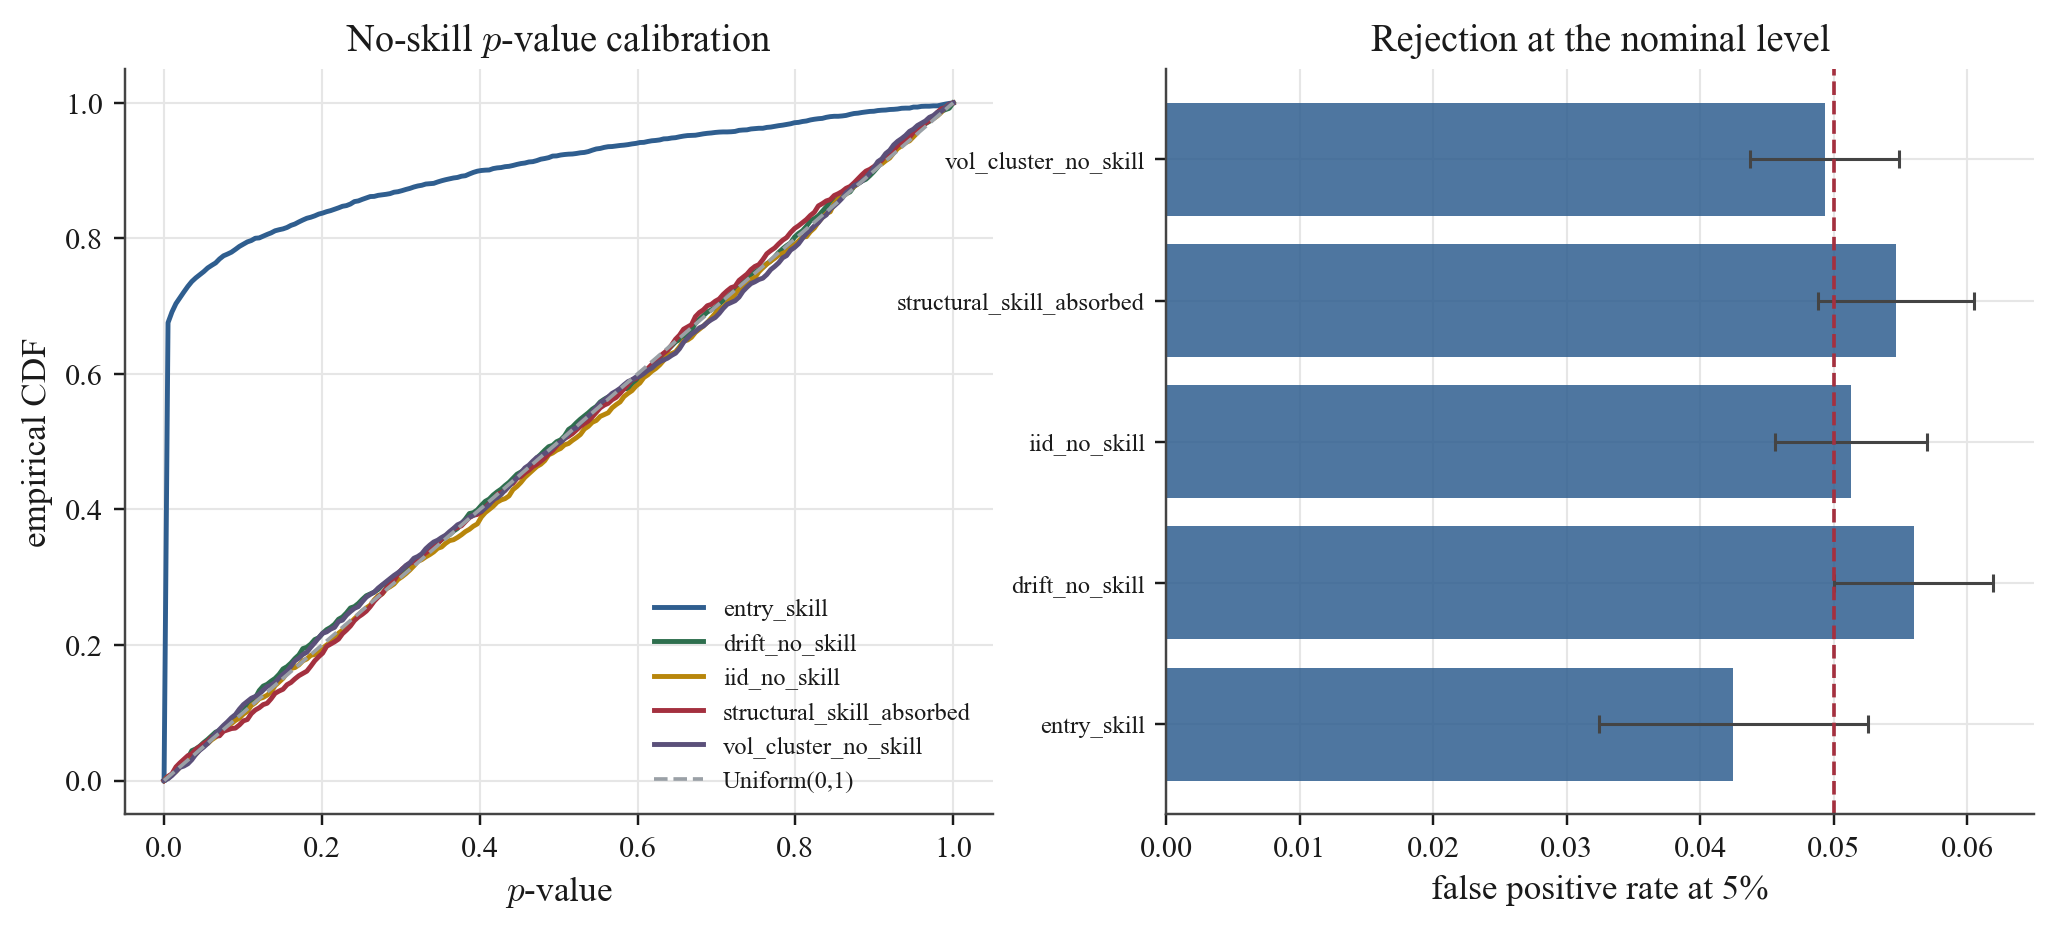
\includegraphics[width=0.95\textwidth]{synthetic_type1_calibration.png}
\caption{Synthetic p-value calibration under no-entry-skill worlds. The left panel compares empirical p-value CDFs with the uniform benchmark; the right panel reports false positive rates at the 5\% level.}
\label{fig:synthetic_calibration}
\end{figure}

Power rises monotonically with the injected entry signal. With no signal the 5\% rejection estimate is $0.043$ in the power-curve sample; at 5 basis points per event bar it rises to $0.130$, at 10 basis points to $0.475$, at 20 basis points to $0.925$, and at 35 basis points to $1.000$. The method therefore detects sufficiently strong entry placement while preserving the warning that weak signals and small trade counts can be underpowered.

\begin{figure}[htbp]
\centering
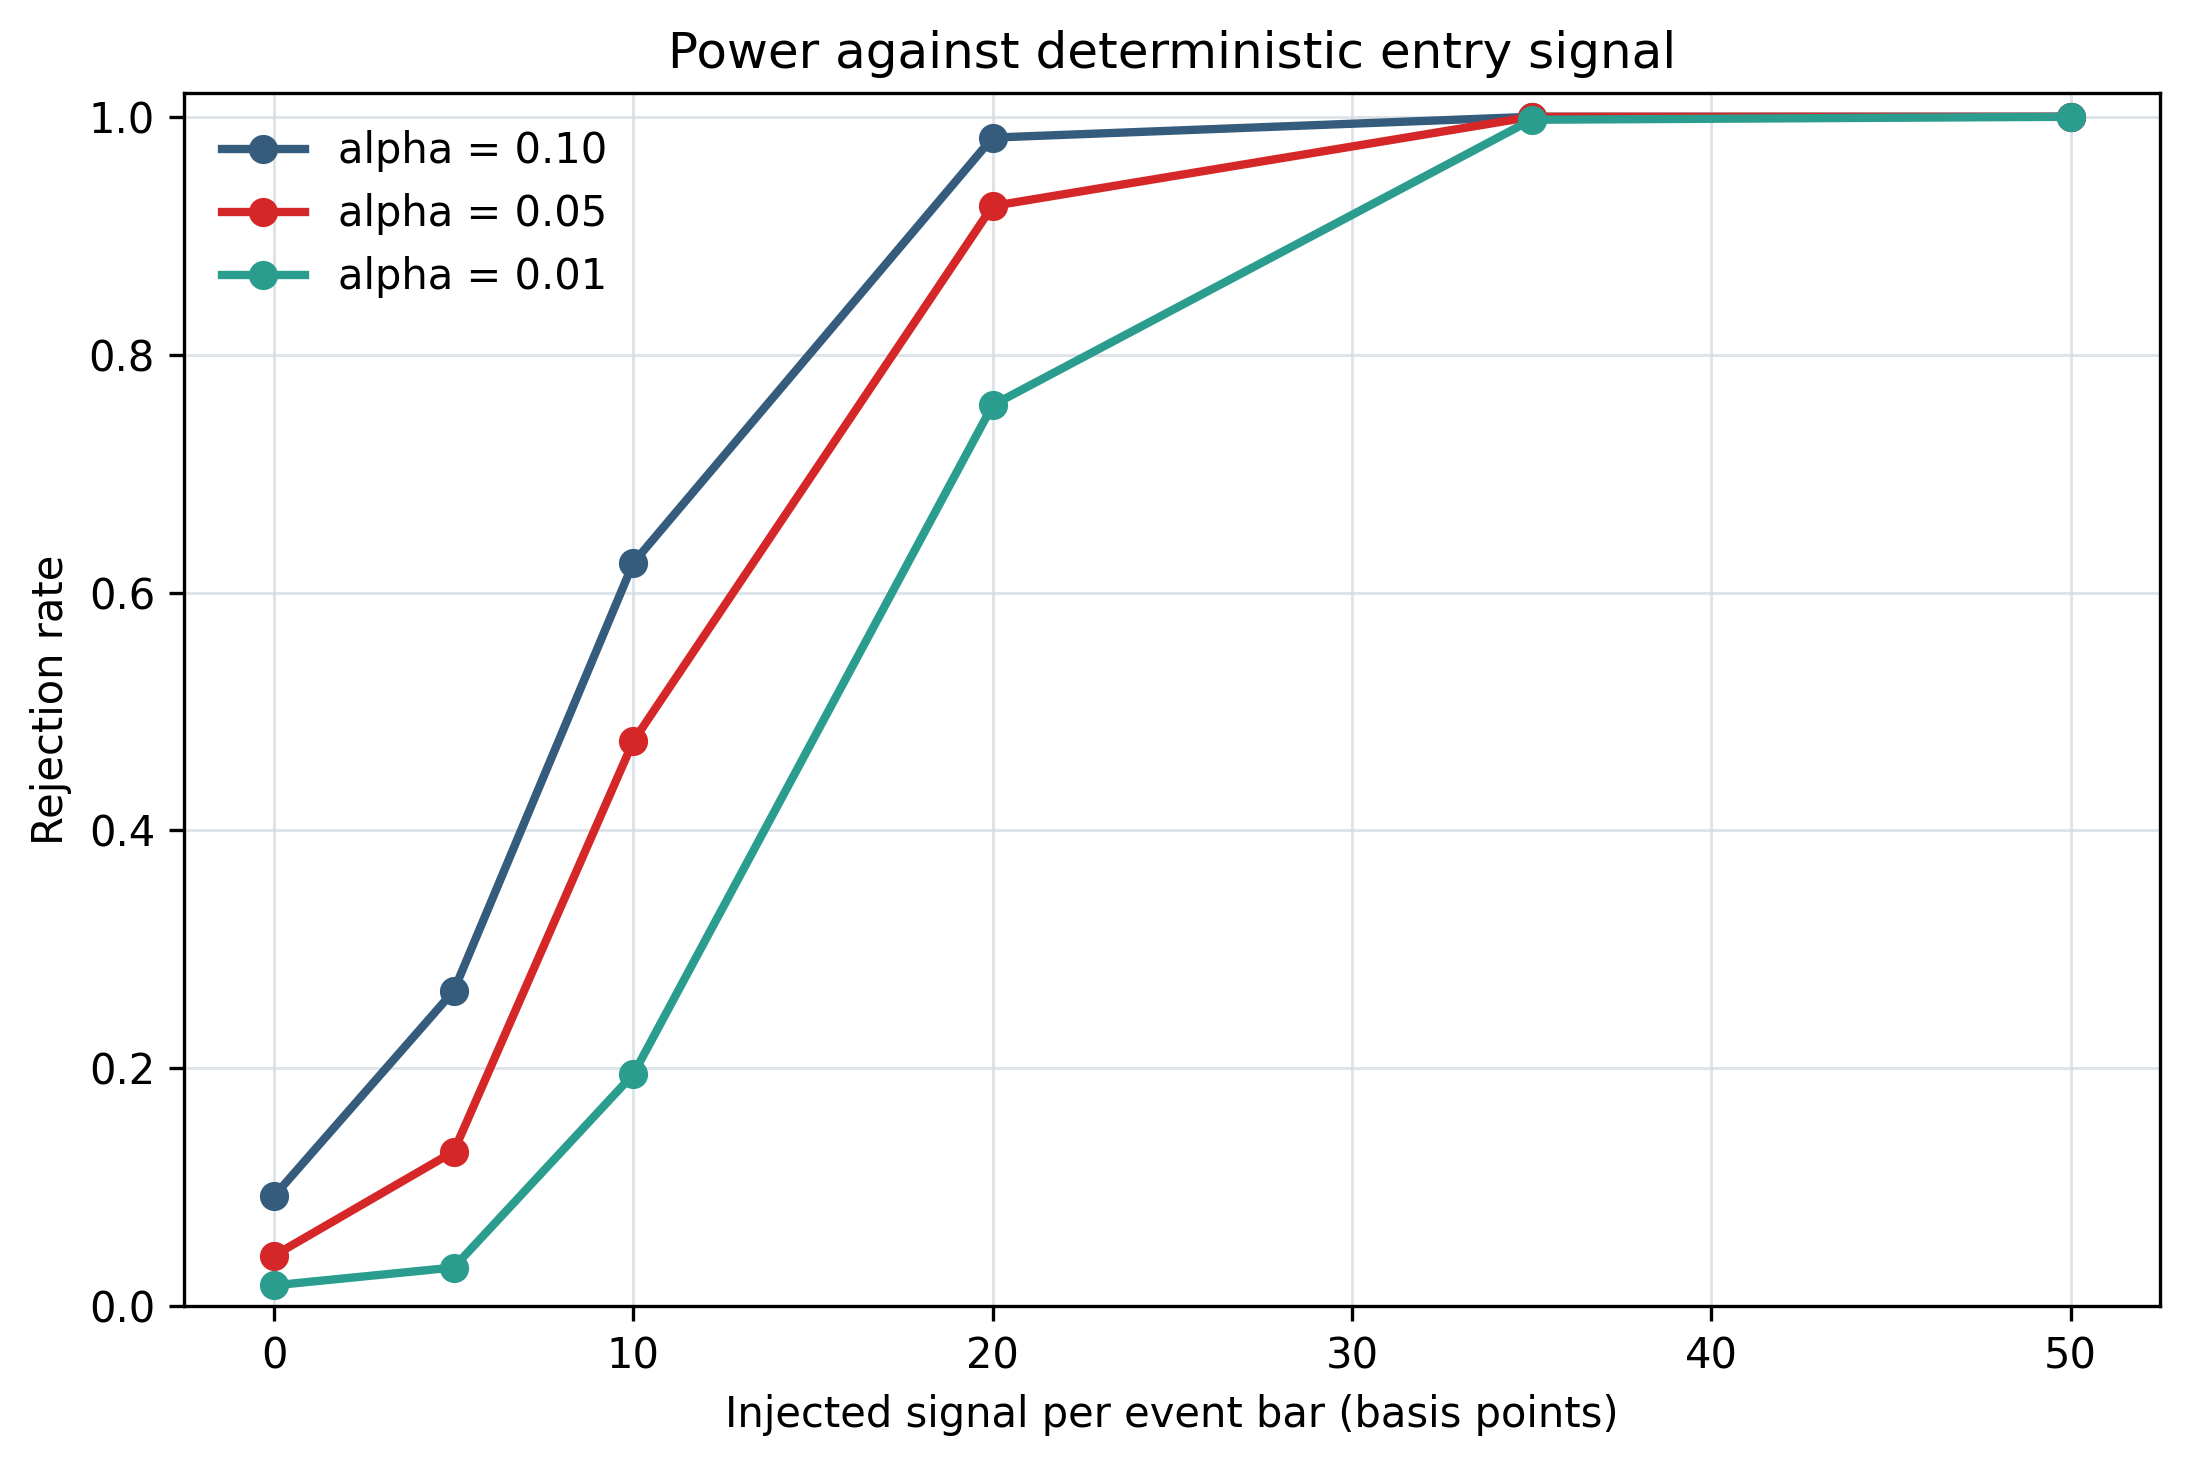
\includegraphics[width=0.78\textwidth]{synthetic_power_curve.png}
\caption{Synthetic power curve for deterministic entry signal. Signal strength is measured in basis points added to each event-window return bar.}
\label{fig:synthetic_power}
\end{figure}

\subsection{Positive control: detecting injected skill on the real price path}
\label{sec:positive-control}

The synthetic worlds above establish calibration and power in artificial data. A sharper question is whether the test can ever reject on the \emph{real} GC=F price path, or whether the null verdict merely reflects a procedure incapable of rejection. We answer this directly with a positive control. On the actual GC=F open-price series we construct a long-only strategy of $N=30$ trades, each held $d=10$ open-to-open bars at equal weight, and we control its timing quality with a skill parameter $\alpha\in[0,1]$: a fraction $\alpha$ of entries are placed, using forward information, in the top quintile of the $d$-bar forward-return distribution available in their local feasible window (``good timing''), and the remaining $1-\alpha$ are placed by an unbiased random non-overlapping draw (``luck''). At $\alpha=0$ the strategy carries no timing skill; at $\alpha=1$ every entry is well timed. The oracle uses future information \emph{by construction}---it is an injected control, not a claim that any gold trader possesses such foresight. Each realized schedule is then scored against the paper's own structure-preserving null (Section~\ref{sec:spr}), which preserves the realized durations and gap multiset and randomizes only placement, thereby destroying the oracle alignment. Realized statistic and null are computed with execution-cost simulation disabled so the two differ only in placement; we run $100$ seeds per skill level at $M=5{,}000$ simulations.

\begin{table}[H]
\centering
\caption{Positive control on the real GC=F price path: detection of injected entry-placement skill. A fraction $\alpha$ of the $30$ long trades are placed with genuine foresight; the rest are random. Each row averages $100$ seeds at $M=5{,}000$ structure-preserving null simulations. ``Reject @ 5\%'' and ``Strong rate'' are the shares of seeds with $p\le0.05$ and with a Strong-skill classification respectively.}
\label{tab:positive_control}
{\small
\renewcommand{\arraystretch}{1.12}
\begin{adjustbox}{max width=\textwidth}
\begin{tabular}{@{}rrrrrrr@{}}
\toprule
Injected skill $\alpha$ & Mean $p$ & Median $p$ & Mean percentile & Mean $\mathrm{RCSI}_z$ & Reject @ 5\% & Strong rate \\
\midrule
0.00 & 0.495 & 0.530 & \phantom{0}50.5 & 0.03 & 0.03 & 0.03 \\
0.20 & 0.158 & 0.091 & \phantom{0}84.2 & 1.38 & 0.35 & 0.22 \\
0.40 & 0.021 & 0.002 & \phantom{0}98.0 & 2.91 & 0.88 & 0.81 \\
0.60 & 0.002 & $<0.001$ & \phantom{0}99.8 & 4.46 & 0.99 & 0.98 \\
0.80 & $<0.001$ & $<0.001$ & 100.0 & 5.84 & 1.00 & 1.00 \\
1.00 & $<0.001$ & $<0.001$ & 100.0 & 7.23 & 1.00 & 1.00 \\
\bottomrule
\end{tabular}
\end{adjustbox}
}
\par\vspace{0.5em}
\begin{minipage}{0.95\textwidth}
\centering
\footnotesize\emph{Notes.} $\alpha=0$ is a genuine no-skill control: it sits at the null median ($50$th percentile, $\mathrm{RCSI}_z\approx0$) and rejects within Monte Carlo error of the nominal $5\%$ rate. Median $p$ reaches the $1/(M+1)$ resolution floor at high $\alpha$.
\end{minipage}
\end{table}

The control behaves exactly as a sound test should (Table~\ref{tab:positive_control}, Figure~\ref{fig:pc_curve}). With no injected skill the test sits squarely at the null median---$50.5$th percentile, mean $\mathrm{RCSI}_z$ of $0.03$---and rejects within Monte Carlo error of the nominal $5\%$ rate. As genuine timing skill is added, power rises monotonically: by $\alpha=0.4$, $88\%$ of seeds reject and $81\%$ are classified Strong, and by $\alpha\ge0.8$ every seed is Strong, with mean $\mathrm{RCSI}_z$ climbing from $2.9$ at $\alpha=0.4$ to $7.2$ at $\alpha=1$. Figure~\ref{fig:pc_hist} shows a single well-timed run ($\alpha=1$): its realized cumulative return falls far in the upper tail of the structure-preserving null ($p\approx0.0002$, $\mathrm{RCSI}_z\approx8$), with no random placement of the same trades coming close. The null result reported for the real strategies is therefore not an artifact of a powerless test on real prices: when entry-placement skill is genuinely present on the GC=F path, this exact procedure detects it decisively.

\begin{figure}[htbp]
\centering
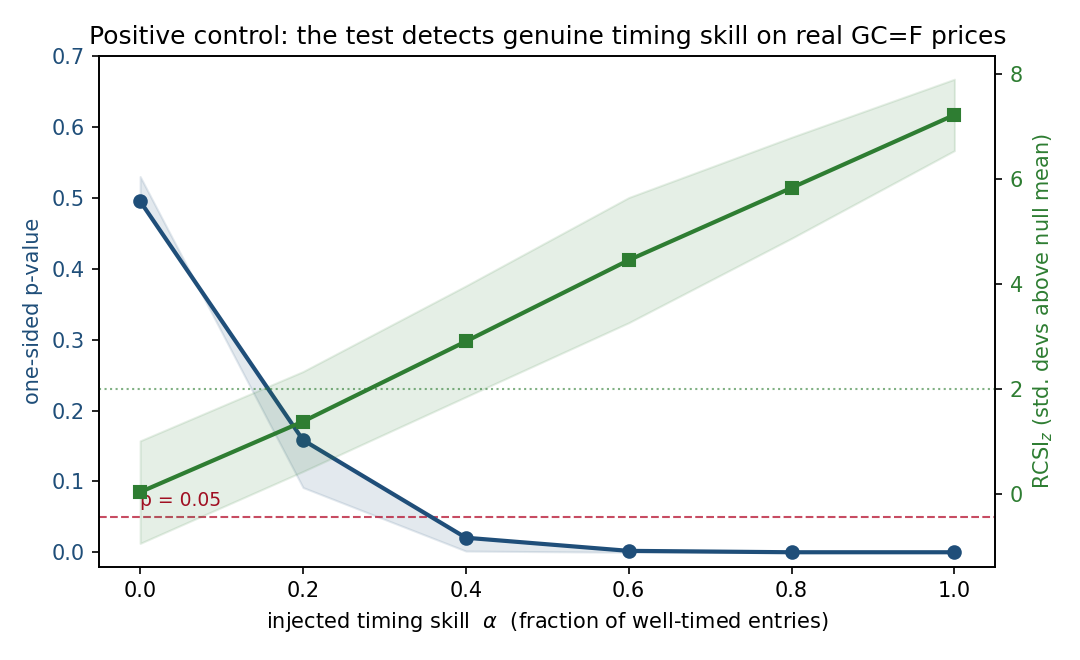
\includegraphics[width=0.82\textwidth]{positive_control_skill_curve.png}
\caption{Positive control on real GC=F prices. As injected timing skill $\alpha$ increases, the mean one-sided $p$-value (blue, left axis) collapses below $0.05$ and the mean $\mathrm{RCSI}_z$ (green, right axis) rises well past $2$. Bands show the seed dispersion. At $\alpha=0$ the test behaves like the null.}
\label{fig:pc_curve}
\end{figure}

\begin{figure}[htbp]
\centering
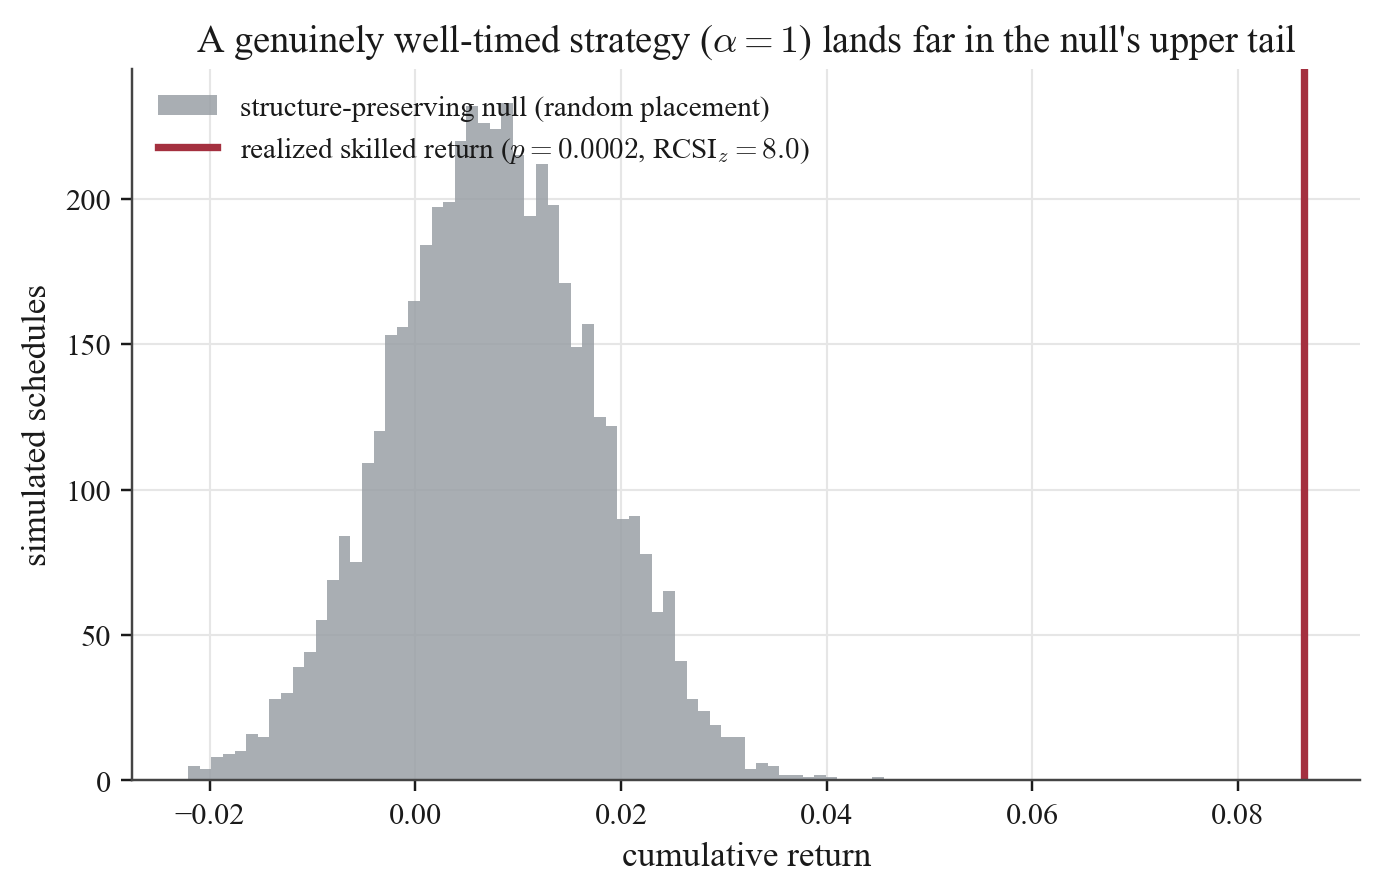
\includegraphics[width=0.82\textwidth]{positive_control_example_histogram.png}
\caption{A single genuinely well-timed strategy ($\alpha=1$) on the real GC=F path. The realized cumulative return (red) lies far beyond the entire structure-preserving null distribution of the same trades placed at random ($p\approx0.0002$, $\mathrm{RCSI}_z\approx8$).}
\label{fig:pc_hist}
\end{figure}

\subsection{Detecting realistic and imperfect signals}
\label{sec:realistic-signals}

The oracle of the previous subsection uses future information by construction; it certifies that the test \emph{can} reject, but a referee rightly asks whether it detects the noisy, imperfect signals a real strategy would use. We answer this on the same GC=F path by driving entry placement with signals of controlled quality, summarized by $\rho$, the Pearson correlation between the entry signal and the $d$-bar forward return. A strategy enters at its top-$N$ signal bars (mutually non-overlapping); the realized schedule is scored against the same structure-preserving null. The oracle is the limiting case $\rho\to1$; $\rho=0$ is no skill.

Figure~\ref{fig:signal_curve} reports power as a function of realized signal quality, using a noisy signal $s=z(f)+\lambda\varepsilon$ whose correlation with the forward return $f$ is tuned across a grid. The rejection rate rises smoothly from the nominal $5\%$ level at $\rho\approx0$ ($\rho=0.0001$: reject rate $0.00$, mean $p=0.52$) to certain detection by $\rho\approx0.20$ (reject rate $1.00$, mean $p=0.005$), passing through partial power at $\rho\approx0.10$ (reject rate $0.48$, mean $p=0.099$). The minimum detectable signal--return correlation for $80\%$ power is therefore roughly $\rho\approx0.15$ at the GC=F trade counts---a concrete, interpretable sensitivity that the bare oracle does not provide and that matches the $\sqrt{N_s}$ scaling of Section~\ref{sec:theory}.

\begin{figure}[htbp]
\centering
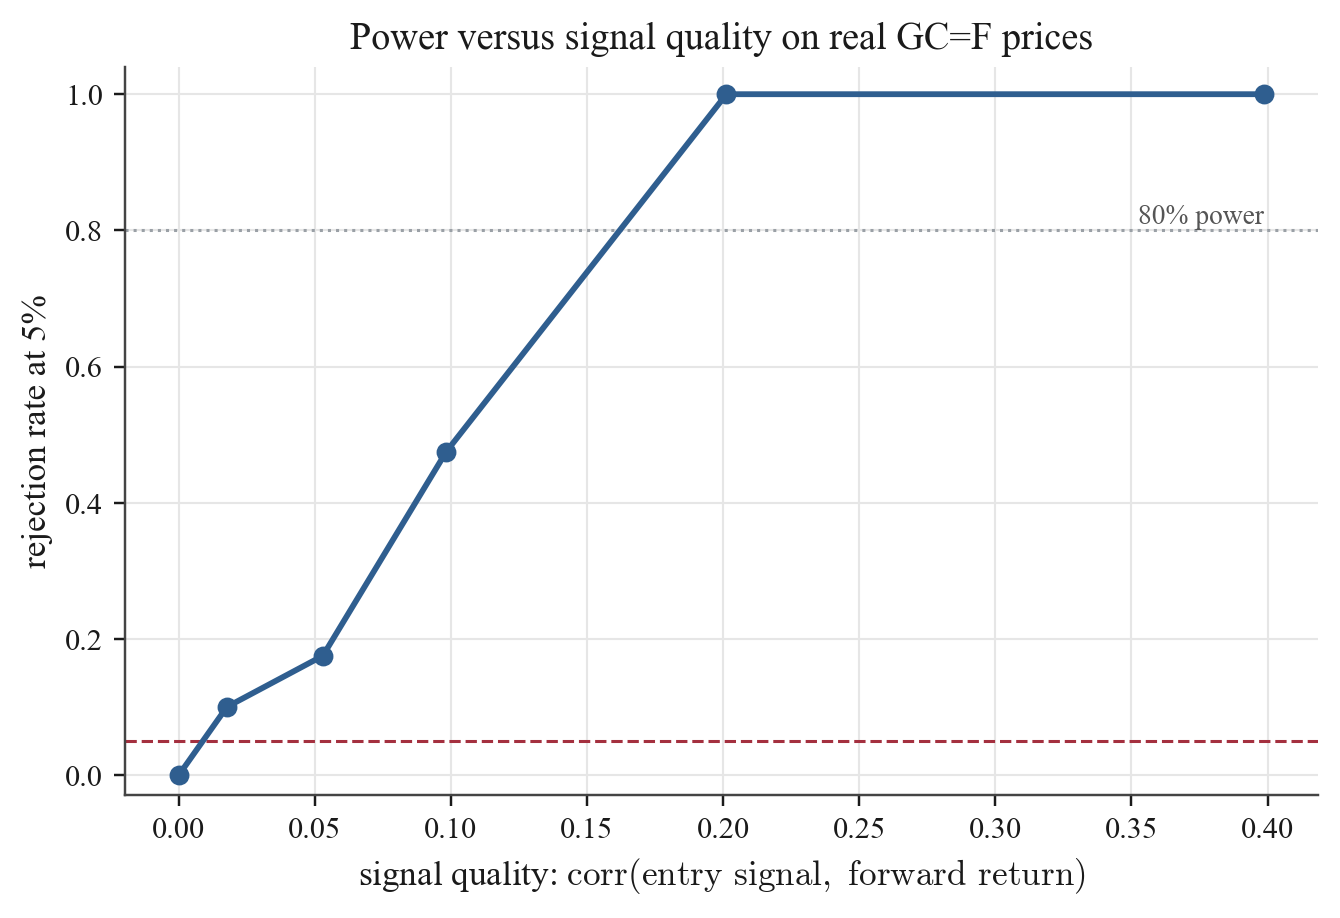
\includegraphics[width=0.74\textwidth]{positive_control_signal_curve.png}
\caption{Power versus signal quality on the real GC=F path. Each point averages $40$ seeds at $M=5{,}000$; the horizontal lines mark the nominal $5\%$ level and $80\%$ power. Rejection rises smoothly with the realized signal--forward-return correlation, giving a minimum detectable correlation of roughly $0.15$.}
\label{fig:signal_curve}
\end{figure}

Detection does not depend on foresight or on a particular signal-generating process. Table~\ref{tab:signal_mechanisms} applies the test to four mechanisms: a noisy oracle, an AR(1)-smoothed signal, a regime-conditional signal (skill only inside calm regimes), and a \emph{causal} momentum signal (trailing return, using no future information). The three signals with positive realized quality are detected in proportion to their correlation---regime-conditional ($\rho=0.27$) most strongly, then AR(1) ($\rho=0.16$) and the noisy oracle ($\rho=0.10$). The momentum signal is the most instructive: on gold at this horizon trailing momentum is \emph{anti}-correlated with the forward return ($\rho=-0.07$, a mean-reverting tendency), so it times entries poorly, and the test correctly assigns it no skill---indeed it sits well below the null median. The procedure responds to the realized informativeness of a signal, not to the analyst's intent or to whether the signal happens to be causal.

\begin{table}[H]
\centering
\caption{Detection across signal-generating processes on the real GC=F path (target correlation $0.10$ for the calibrated signals; $40$ seeds at $M=5{,}000$). $\bar\rho$ is the mean realized signal--forward-return correlation.}
\label{tab:signal_mechanisms}
{\small
\renewcommand{\arraystretch}{1.12}
\begin{adjustbox}{max width=\textwidth}
\begin{tabular}{@{}lrrrr@{}}
\toprule
Signal-generating process & $\bar\rho$ & Mean $p$ & Reject @ 5\% & Mean $\mathrm{RCSI}_z$ \\
\midrule
Regime-conditional (calm-only skill) & \phantom{-}0.27 & 0.054 & 0.85 & \phantom{-}2.42 \\
AR(1)-smoothed signal & \phantom{-}0.16 & 0.051 & 0.63 & \phantom{-}2.15 \\
Noisy oracle & \phantom{-}0.10 & 0.107 & 0.40 & \phantom{-}1.49 \\
Momentum, causal (trailing return) & $-0.07$ & 1.000 & 0.00 & $-4.82$ \\
\bottomrule
\end{tabular}
\end{adjustbox}
}
\par\vspace{0.5em}
\begin{minipage}{0.95\textwidth}
\centering
\footnotesize\emph{Notes.} Calibrated signals (noisy oracle, AR(1)) target a modest correlation of $0.10$; the regime-conditional and causal-momentum signals realize whatever correlation the data produce. A causal momentum rule is anti-predictive for entry timing on gold at the $10$-bar horizon, and is correctly classified below the null median rather than as skill.
\end{minipage}
\end{table}

\section{Empirical results}

\subsection{Central results table}

Table \ref{tab:main} is the paper's central results table. It combines the verified outputs:
\begin{itemize}
\item final cumulative returns and sample window from the equity-curve figure (Figure~\ref{fig:equity_curves}),
\item trade counts from each strategy-specific Monte Carlo distribution figure (Figures~\ref{fig:mc_trend_pullback}--\ref{fig:mc_random}),
\item $p$-values, percentiles, $\mathrm{RCSI}_z$, and verdicts from the supplied Skill vs Luck Summary output image,
\item RCSI robustness (mean $\pm$ SD across seeds) from the robustness chart (Figure~\ref{fig:rcsi_robust}).
\end{itemize}

\clearpage
\begin{table}[p]
\centering
\caption{GC=F daily panel. Verified strategy outcomes and skill diagnostics (three-decimal formatting where appropriate).}
\label{tab:main}
{\small
\renewcommand{\arraystretch}{1.15}
\setlength{\tabcolsep}{5pt}
\begin{adjustbox}{max width=\textwidth}
\begin{tabular}{@{}lrrrrrrl@{}}
\toprule
Strategy & Cum.\ return & Trades & RCSI (mean$\pm$SD) & $p$-value & Percentile & $\mathrm{RCSI}_z$ & Verdict \\
\midrule
Trend Pullback      & 0.083 &  77 & $-0.361\pm0.005$ & 0.870 & 13.0 & -1.03 & Below null median \\
Breakout Vol+Mom    & 0.297 &  46 & $\phantom{-}0.158\pm0.003$ & 0.176 & 82.4 & \phantom{-}0.91 & Weak skill \\
Mean Rev Vol Filter & -0.010 & 13 & $-0.029\pm0.001$ & 0.662 & 33.8 & -0.44 & Random or luck \\
Validation AVM      & 0.219 &  35 & $\phantom{-}0.059\pm0.003$ & 0.345 & 65.5 & \phantom{-}0.32 & Random or luck \\
ADX Trend           & 0.803 & 110 & $\phantom{-}0.387\pm0.005$ & 0.141 & 85.9 & \phantom{-}1.08 & Weak skill \\
Oversold Reversion  & 0.082 &  30 & $\phantom{-}0.034\pm0.001$ & 0.341 & 65.9 & \phantom{-}0.35 & Random or luck \\
Squeeze Breakout    & 0.065 &   4 & $\phantom{-}0.055\pm0.000$ & 0.053 & 94.7 & \phantom{-}1.50 & Weak skill \\
Connors RSI2        & 0.118 &  41 & $\phantom{-}0.094\pm0.001$ & 0.143 & 85.7 & \phantom{-}1.07 & Weak skill \\
Donchian Reentry    & 0.071 &  60 & $-0.088\pm0.003$ & 0.647 & 35.3 & -0.46 & Random or luck \\
Turn-of-Month       & 0.323 & 141 & $\phantom{-}0.144\pm0.003$ & 0.234 & 76.7 & \phantom{-}0.65 & Random or luck \\
Random              & 0.601 & 215 & $-0.103\pm0.523$ & 0.710 & 29.0 & -0.64 & Below null median \\
\midrule
Buy \& Hold (benchmark) & 14.670 & --- & --- & --- & --- & --- & Benchmark \\
\bottomrule
\end{tabular}
\end{adjustbox}
}
\par\vspace{0.75em}
\begin{minipage}{0.95\textwidth}
\centering
\footnotesize\emph{Notes.} Cum.\ returns are the final cumulative returns shown in the equity-curve figure for the common window 2002-03-04 to 2026-04-02. Trades are the counts reported in the strategy-specific Monte Carlo distribution captions. RCSI is reported as mean $\pm$ SD across outer-run seeds from the robustness figure (outer runs = 100, simulations per run = 5{,}000, transaction cost = 0.000470). The verdict and ($p$-value, percentile, $\mathrm{RCSI}_z$) reproduce the classifier-aligned values from the supplied Skill vs Luck Summary output image.
\end{minipage}
\end{table}
\clearpage

Three patterns stand out. First, profit is common. Ten of the eleven strategies report positive final cumulative return, while Mean Rev Vol Filter is slightly negative at $-0.010$. The buy-and-hold benchmark reaches $14.670$, showing how much long-horizon appreciation existed in the sample. Second, strong entry-placement evidence is rare under the structure-preserving null. The p-value chart (Figure~\ref{fig:pval_by_strategy}) marks the conventional $p=0.05$ threshold, and no strategy crosses it. Squeeze Breakout comes closest at $p=0.053$. Third, the classifier assigns no moderate or strong skill to any strategy in the panel. Four strategies classify as weak skill, five as random or luck, and two below the null median (Figure~\ref{fig:rcsi_by_strategy}).

\subsection{Comparison to alternative nulls}

To show what the structure-preserving null adds, the empirical panel is re-evaluated against two return-based baselines. The shuffled-return null replays each realized trade schedule on IID permutations of the observed open-to-open returns. The stationary-bootstrap null replays the same schedules on stationary-bootstrap return paths with mean block length 20 bars. Both preserve the realized trade geometry but replace the realized price path. The comparison is run with fixed transaction cost $c=0.000470$, $M=5{,}000$ simulations per strategy and method (Table~\ref{tab:null_benchmark}).

\begin{table}[H]
\centering
\caption{Comparison of null methods on the GC=F strategy panel.}
\label{tab:null_benchmark}
{\small
\renewcommand{\arraystretch}{1.12}
\begin{adjustbox}{max width=\textwidth}
\begin{tabular}{@{}lccccrrl@{}}
\toprule
Null method & Path & Geometry & Snooping & Entry test & Median $p$ & Reject @ 5\% & Closest strategy \\
\midrule
Structure-preserving schedule & Yes & Yes & No & Yes & 0.348 & 0 & Squeeze Breakout ($p=0.058$) \\
Shuffled returns & No & Yes & No & No & 0.293 & 1 & Squeeze Breakout ($p=0.030$) \\
Stationary bootstrap returns & No & Yes & No & No & 0.309 & 1 & Squeeze Breakout ($p=0.025$) \\
\bottomrule
\end{tabular}
\end{adjustbox}
}
\par\vspace{0.5em}
\begin{minipage}{0.95\textwidth}
\centering
\footnotesize\emph{Notes.} ``Path'' indicates whether the realized price path is preserved. ``Geometry'' indicates whether realized entries, exits, holding periods, weights, and directions are retained or structurally matched. ``Snooping'' indicates whether the method controls strategy-selection search across the panel; none of these within-strategy diagnostics does so. Method-specific Benjamini--Hochberg adjustment leaves no strategy significant at 5\% under any method. The structure-preserving-schedule row is computed by the independent benchmark-comparison harness ($M=5{,}000$, separate seed); its Squeeze Breakout $p=0.058$ and median $p=0.348$ differ from the $0.053$ and $0.341$ of Table~\ref{tab:main} only by Monte Carlo seed variation.
\end{minipage}
\end{table}

\begin{figure}[htbp]
\centering
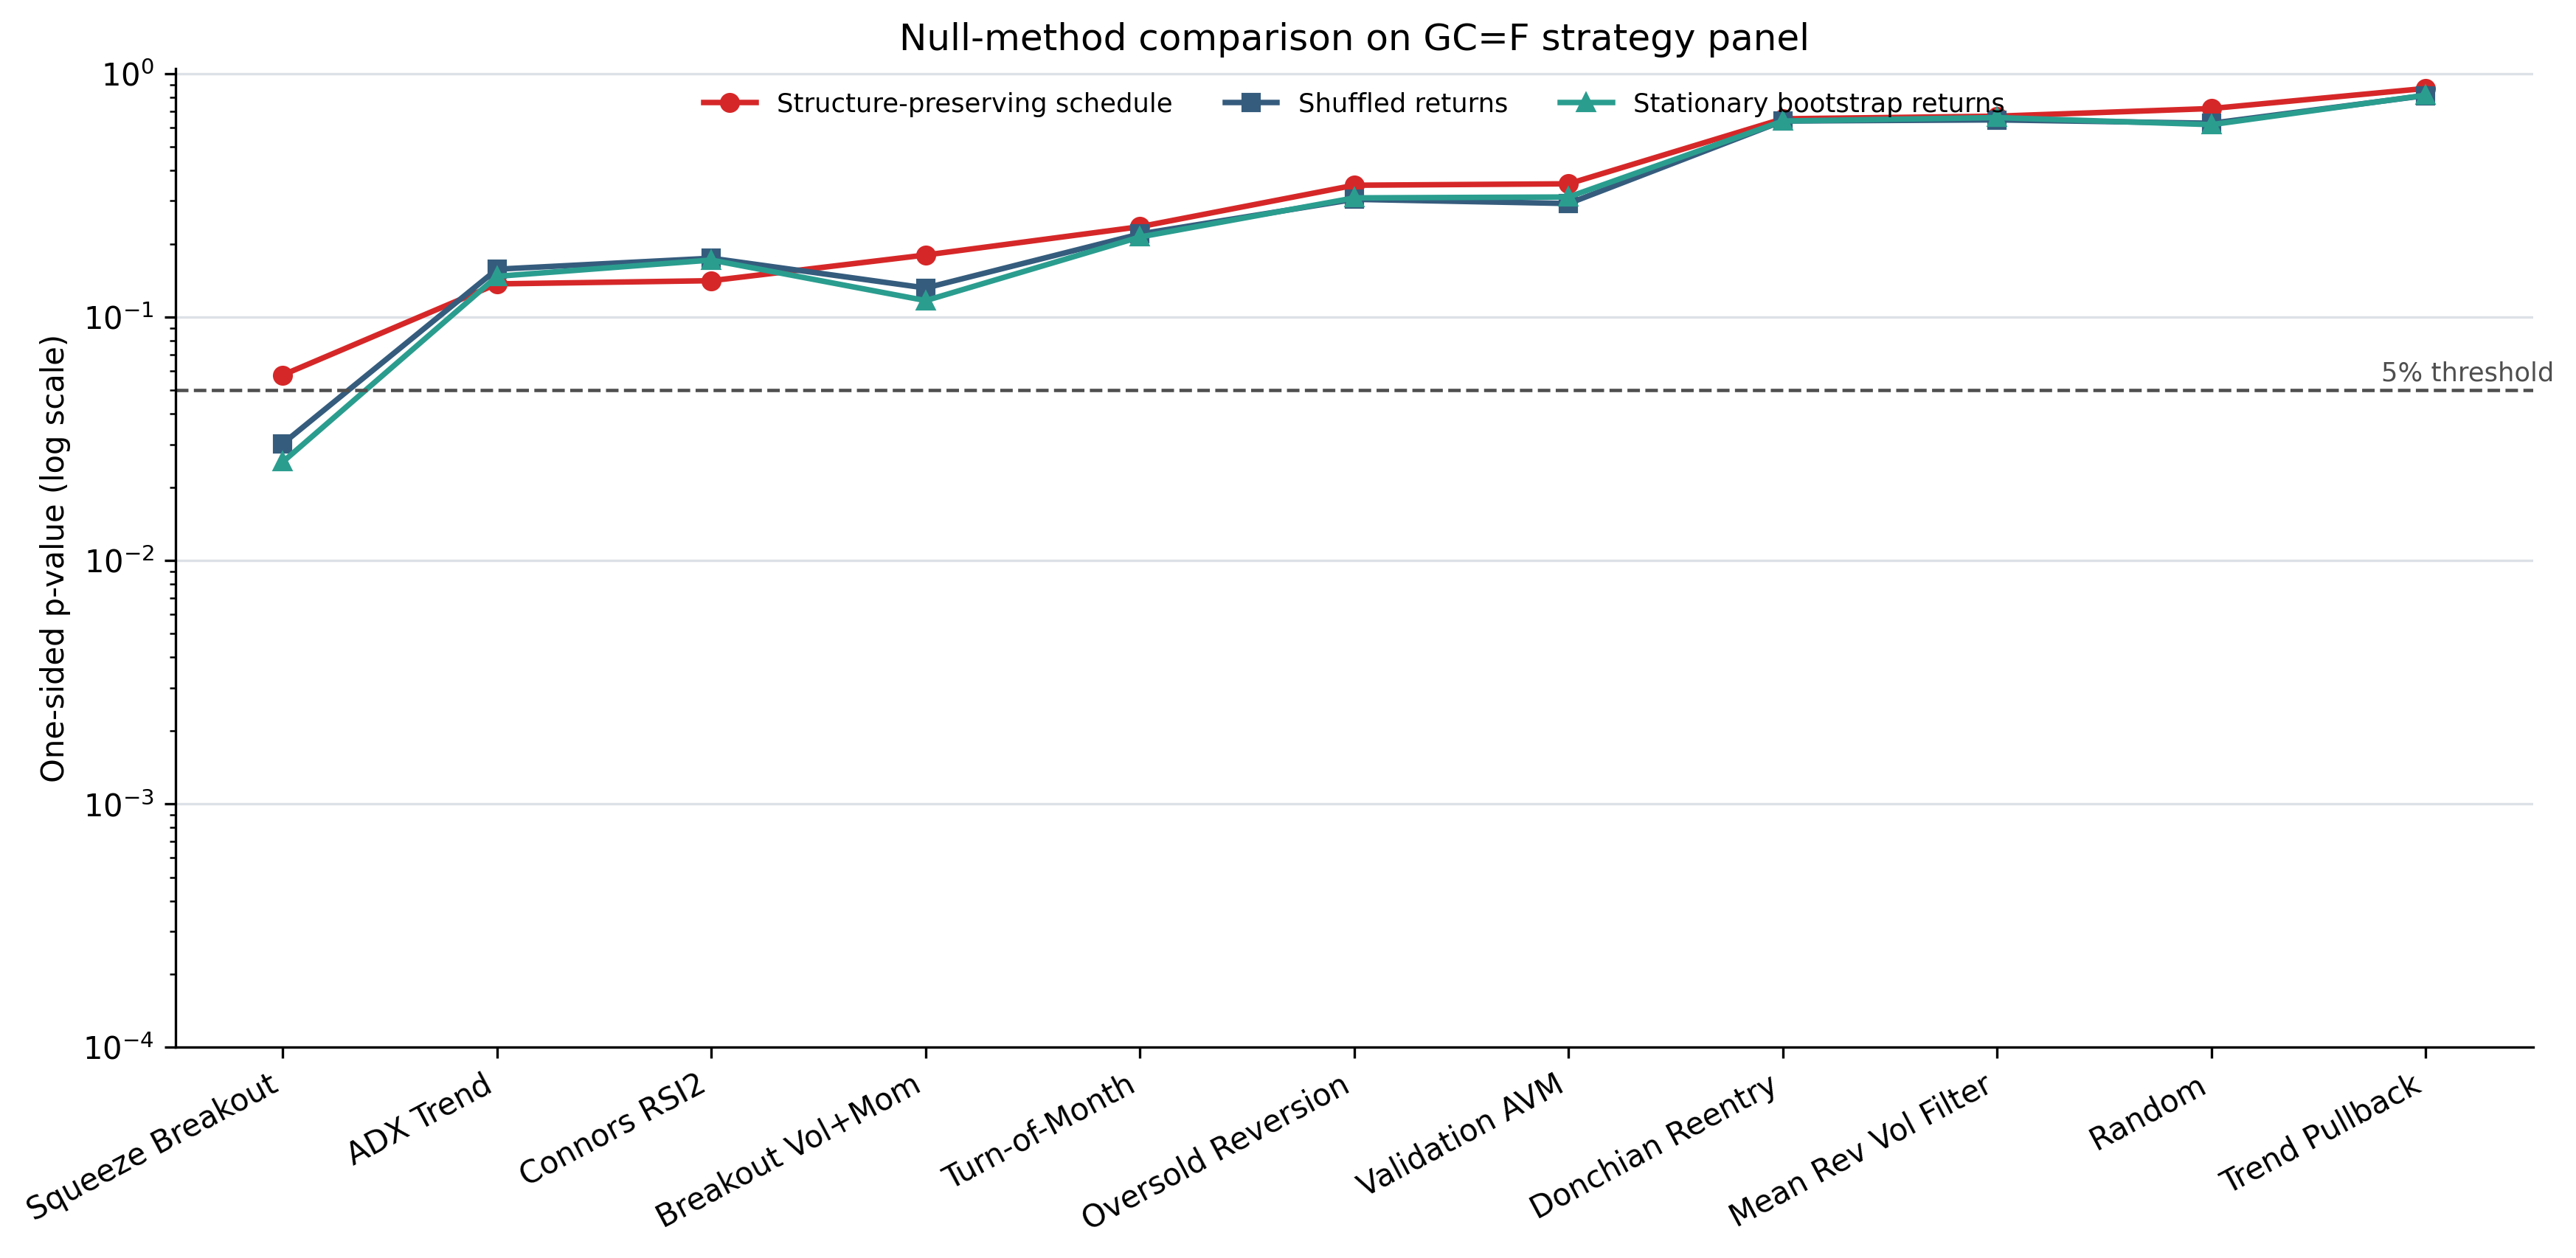
\includegraphics[width=0.95\textwidth]{null_method_comparison.png}
\caption{One-sided p-values under structure-preserving schedule randomization, shuffled returns, and stationary-bootstrap returns.}
\label{fig:null_method_comparison}
\end{figure}

The comparison clarifies the estimand (Figure~\ref{fig:null_method_comparison}). The return-based nulls make Squeeze Breakout significant at the raw 5\% level, while the structure-preserving schedule null leaves it just above threshold. This is not a contradiction. The return nulls ask whether the realized trade schedule performs unusually well relative to synthetic return histories. The structure-preserving schedule null asks whether the realized entry placement is unusually good on the actual price path, conditional on the same exposure geometry. A strategy can look exceptional against resampled returns yet remain only marginal against randomized placement on the realized path. For this paper's question, the latter comparison is the stricter and more directly targeted diagnostic.

The benchmark also states what remains unsolved. None of the three methods controls for the fact that the strategy panel itself was selected by the researcher. White's Reality Check and Hansen's SPA test are therefore not replaced by the proposed diagnostic; they answer the complementary between-strategy data-snooping question.

\subsection{Schedule-measure sensitivity and leading-gap robustness}
\label{sec:schedule-sensitivity}

Section~\ref{sec:spr} argued that the schedule measure is part of the null hypothesis rather than a property of the data. We make that concrete by re-evaluating the entire eleven-strategy panel---on the same realized trade logs and the same price path---under two perturbations of the primary gap-permutation measure. The first is a \emph{leading-gap restriction} that forbids the first simulated entry from being placed inside the universal $200$-bar signal warm-up, the region in which a long-lookback rule could not yet have produced a signal. The second is the \emph{context-matched} measure of Table~\ref{tab:schedule_measures}, which additionally restricts random entries to bars whose volatility context resembles the realized entries. Each variant uses $M=5{,}000$ simulations and the same seed protocol; the gap-permutation column reproduces Table~\ref{tab:main} exactly.

\begin{table}[H]
\centering
\caption{Schedule-measure sensitivity. One-sided Monte Carlo $p$-values for the GC=F panel under the primary gap-permutation measure, a leading-gap restriction (first entry beyond the $200$-bar warm-up), and the context-matched measure. Daggers mark $p\le 0.05$.}
\label{tab:schedule_sensitivity}
{\small
\renewcommand{\arraystretch}{1.12}
\setlength{\tabcolsep}{7pt}
\begin{adjustbox}{max width=\textwidth}
\begin{tabular}{@{}lrrr@{}}
\toprule
Strategy & Gap-permutation $p$ & Leading-gap $\ge 200$ $p$ & Context-matched $p$ \\
\midrule
Trend Pullback      & 0.870 & 0.910 & 1.000 \\
Breakout Vol+Mom    & 0.176 & 0.128 & 0.022$^\dagger$ \\
Mean Rev Vol Filter & 0.662 & 0.668 & 0.395 \\
Validation AVM      & 0.345 & 0.303 & 0.993 \\
ADX Trend           & 0.141 & 0.055 & 0.010$^\dagger$ \\
Oversold Reversion  & 0.341 & 0.383 & 0.146 \\
Squeeze Breakout    & 0.053 & 0.100 & 0.030$^\dagger$ \\
Connors RSI2        & 0.143 & 0.155 & ${<}0.001^\dagger$ \\
Donchian Reentry    & 0.647 & 0.671 & 1.000 \\
Turn-of-Month       & 0.234 & 0.320 & 1.000 \\
Random              & 0.710 & 0.713 & 1.000 \\
\midrule
Significant at $5\%$ & 0 of 11 & 0 of 11 & 4 of 11 \\
\bottomrule
\end{tabular}
\end{adjustbox}
}
\end{table}

Table~\ref{tab:schedule_sensitivity} reports two facts. First, the headline is robust to the feasibility concern: restricting the leading gap past the $200$-bar warm-up changes no verdict and crosses no threshold. The largest shift is ADX Trend, which tightens from $0.141$ to a borderline $0.055$ but remains short of $0.05$; every other strategy moves by at most a few points. The absence of entry-placement skill under the gap-permutation null is therefore not an artifact of letting the null place trades in pre-signal bars a real strategy could not have used.

Second, the verdict does not survive a change of schedule measure. The context-matched measure restricts each random entry to bars whose entry-time context---trailing volatility, in five quantile buckets---matches the strategy's realized entries, with non-overlap preserved. On a strongly trending asset this matched pool can earn far more, or far less, than the realized schedule: four strategies reject at the $5\%$ level (Connors RSI2 at $p<0.001$, ADX Trend at $p=0.010$, Breakout Vol+Mom at $p=0.022$, Squeeze Breakout at $p=0.030$) while four others fall to the floor of the null ($p\approx 1$). We do \emph{not} read these four rejections as competing evidence of skill. The neutral gap-permutation measure already rejects none, so the conjunctive standard---significant under every defensible measure---is settled by that column alone. And because the matched pools are narrow, they can mechanically sharpen tails in either direction: a genuine state-conditional volatility-timing edge cannot be separated from a pool artifact here, a disentanglement we leave to future work. The point is the disagreement itself: a timing verdict that flips across two defensible schedule measures establishes the absence of \emph{robust, measure-invariant} entry-placement skill---not its presence---which is the paper's central epistemic claim, now demonstrated within a single asset rather than asserted.

\subsection{Multi-asset walk-forward evidence}

The single-asset GC=F analysis is supplemented with a daily multi-asset walk-forward panel. The universe contains equity ETFs (SPY, QQQ, VOO), single-name equities (AAPL, NVDA, TSM), futures and commodities (GC=F, CL=F, ES=F, NQ=F), foreign exchange (EURUSD=X, GBPUSD=X, AUDUSD=X), and crypto (BTC-USD). Each ticker is split into non-overlapping four-year test windows using 1{,}008-bar folds. A strategy-fold panel is retained only when it produces at least five trades. Each retained panel is evaluated with $M=1{,}000$ structure-preserving null simulations. This extension produces 712 strategy-fold panels (Table~\ref{tab:multi_asset_walk_forward}).

This section is deliberately labeled exploratory. Unlike the GC=F robustness analysis, it uses one outer run per panel rather than repeated seed-level robustness. Its purpose is external-validity pressure: checking whether the main conclusion vanishes once the method leaves gold futures.

\begin{table}[H]
\centering
\caption{Daily multi-asset walk-forward panel summary.}
\label{tab:multi_asset_walk_forward}
{\small
\renewcommand{\arraystretch}{1.12}
\begin{adjustbox}{max width=\textwidth}
\begin{tabular}{@{}lrrrrrrl@{}}
\toprule
Strategy & Panels & Mean $p$ & Mean percentile & Mean $\mathrm{RCSI}_z$ & Sig.\ runs & Outperform null & Classification \\
\midrule
Trend Pullback      & 79 & 0.581 & 42.0 & -0.28 & 1.3\% & 40.5\% & Inconclusive \\
Breakout Vol+Mom    & 76 & 0.595 & 40.6 & -0.31 & 1.3\% & 36.8\% & Inconclusive \\
Mean Rev Vol Filter & 13 & 0.505 & 49.6 & \phantom{-}0.01 & 0.0\% & 38.5\% & Inconclusive \\
Validation AVM      & 73 & 0.599 & 40.2 & -0.33 & 2.7\% & 39.7\% & Inconclusive \\
ADX Trend           & 78 & 0.638 & 36.3 & -0.41 & 2.6\% & 29.5\% & Likely random \\
Oversold Reversion  & 69 & 0.515 & 48.6 & -0.11 & 1.4\% & 52.2\% & Inconclusive \\
Squeeze Breakout    & 24 & 0.691 & 31.0 & -0.59 & 0.0\% & 20.8\% & Likely random \\
Connors RSI2        & 76 & 0.493 & 50.8 & -0.06 & 5.3\% & 52.6\% & Inconclusive \\
Donchian Reentry    & 64 & 0.655 & 34.6 & -0.48 & 3.1\% & 25.0\% & Likely random \\
Turn-of-Month       & 80 & 0.567 & 43.4 & -0.26 & 3.8\% & 38.8\% & Inconclusive \\
Random              & 80 & 0.607 & 39.4 & -0.39 & 2.5\% & 36.3\% & Likely random \\
\bottomrule
\end{tabular}
\end{adjustbox}
}
\par\vspace{0.5em}
\begin{minipage}{0.95\textwidth}
\centering
\footnotesize\emph{Notes.} ``Sig.\ runs'' is the share of retained strategy-fold panels with $p\le0.05$ in the single outer run. ``Outperform null'' is the share whose realized cumulative return exceeds the null median. The run uses cached daily data, $M=1{,}000$ null simulations per panel, one outer run, and minimum five trades per retained panel.
\end{minipage}
\end{table}

\begin{figure}[htbp]
\centering
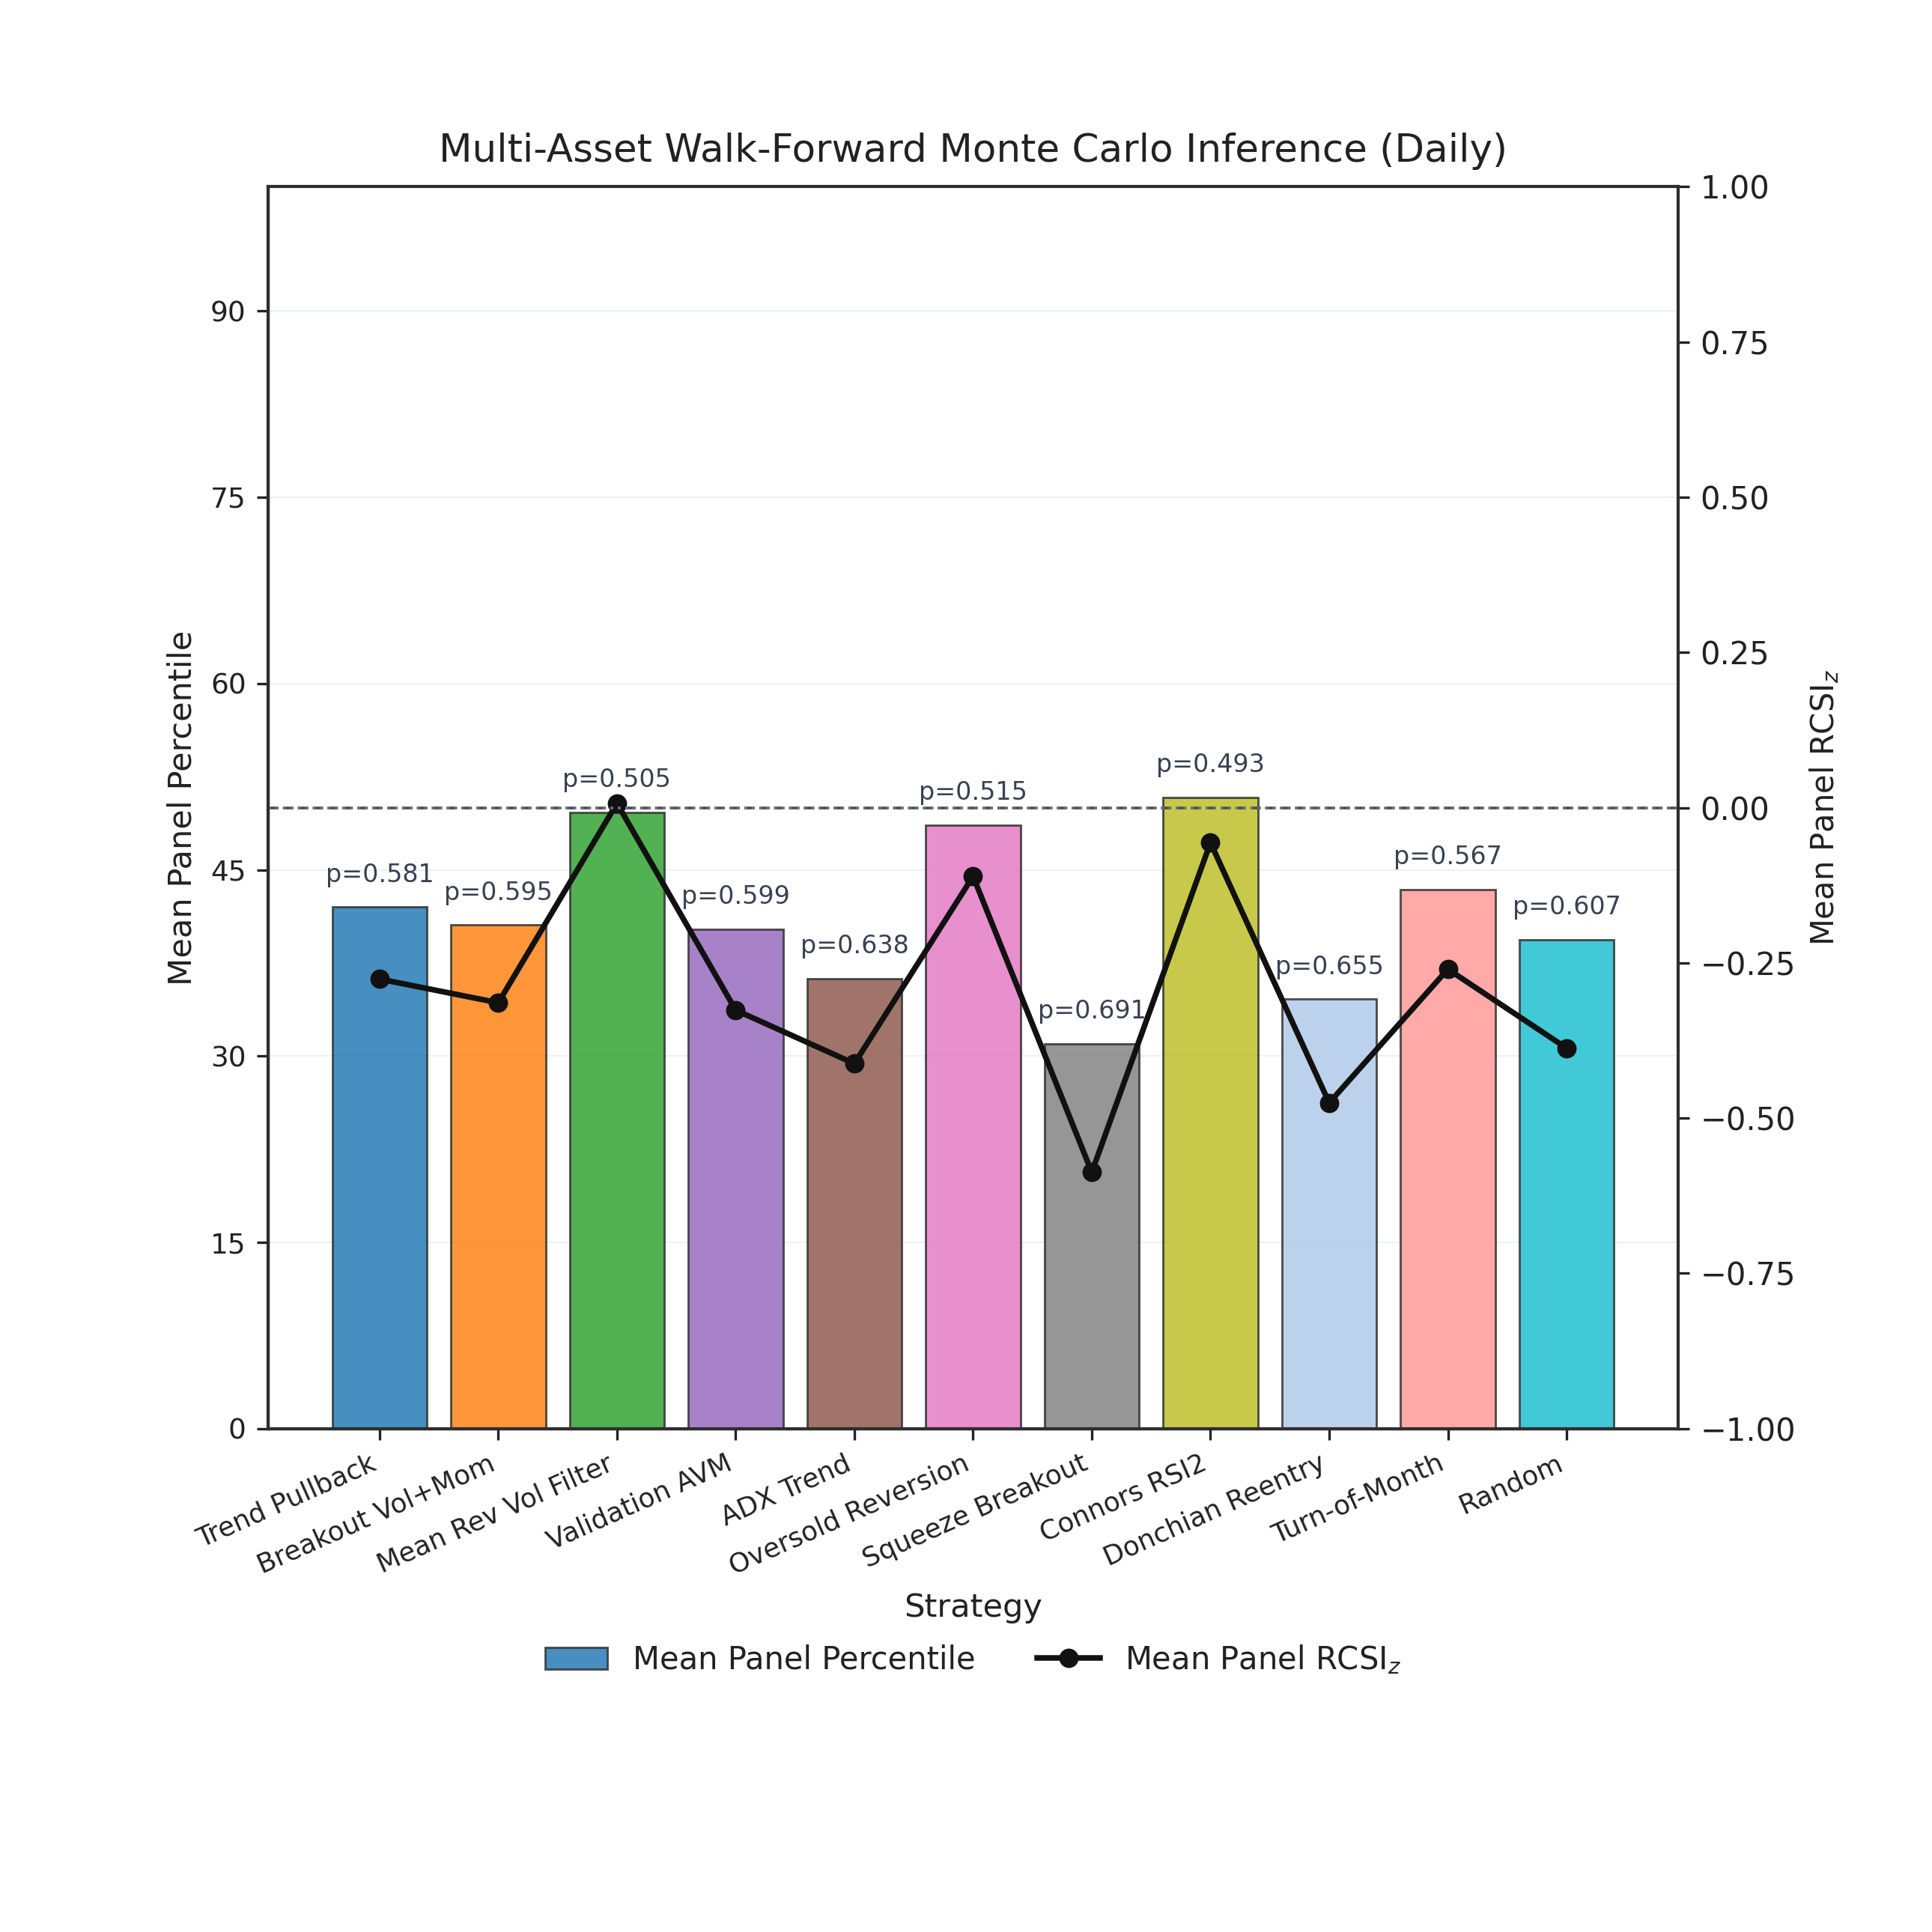
\includegraphics[width=0.95\textwidth]{multi_asset_walk_forward_inference.png}
\caption{Daily multi-asset walk-forward inference summary. Bars report mean panel percentile; the line reports mean panel $\mathrm{RCSI}_z$.}
\label{fig:multi_asset_inference}
\end{figure}

The multi-asset extension does not contradict the GC=F conclusion, though as a single-outer-run panel it is exploratory and cannot independently confirm it; seed-robust inference is established only for GC=F. No strategy has a mean panel $p$-value below 0.49. The strongest cross-panel percentile belongs to Connors RSI2 at 50.8, essentially the null median. Only Connors RSI2 exceeds the null median in more than half of retained panels, and only barely (52.6\%). Strategies that appeared weakly favorable in the single-asset analysis do not become broadly significant once evaluated across asset classes and non-overlapping walk-forward windows (Figure~\ref{fig:multi_asset_inference}).

The result should not be overstated. Because the walk-forward extension uses one outer run per panel, it is not a replacement for the seed-robust GC=F Monte Carlo analysis. It is nevertheless useful evidence against the most serious external-validity objection: the paper is no longer only a gold-futures case study. The broader panel suggests that the profit--skill divergence is not unique to GC=F.

\subsection{Cross-asset breadth under multiplicity control}
\label{sec:cross-asset-multiplicity}

The walk-forward panel above tests temporal stability within a curated set of instruments. A complementary question is what happens when every completed full-sample test is pooled and judged jointly, with explicit correction for the fact that many tests are being run at once. We aggregate the structure-preserving Monte Carlo result for every strategy on every asset for which a completed run exists on disk: $322$ strategy-by-asset tests across $47$ instruments spanning equities, ETFs, futures, commodities, FX, and crypto. This is a search for skill at breadth---if entry-placement edge exists anywhere in this universe, a naive scan would find it---made honest by multiplicity control.

\begin{table}[H]
\centering
\caption{Cross-asset panel under multiplicity control. Every completed structure-preserving test on disk is pooled and corrected jointly. ``Nominal'' counts raw $p\le0.05$; BH and Bonferroni control the false discovery rate and family-wise error rate at $0.05$ across all $322$ tests.}
\label{tab:cross_asset_multiplicity}
{\small
\renewcommand{\arraystretch}{1.12}
\begin{adjustbox}{max width=\textwidth}
\begin{tabular}{@{}lr@{}}
\toprule
Quantity & Value \\
\midrule
Assets / strategy-by-asset tests & $47$ / $322$ \\
Nominal rejections at $p\le0.05$ & $13$ (vs.\ $16.1$ expected by chance) \\
Benjamini--Hochberg discoveries (FDR $0.05$) & $0$ \\
Bonferroni discoveries (FWER $0.05$, threshold $1.55\times10^{-4}$) & $0$ \\
Mean / median panel $p$-value & $0.567$ / $0.580$ \\
KS statistic vs.\ Uniform$(0,1)$ (departure direction) & $0.114$ (conservative) \\
Smallest $p$-value in the panel & $0.0014$ (a \emph{random}-entry baseline) \\
\bottomrule
\end{tabular}
\end{adjustbox}
}
\par\vspace{0.5em}
\begin{minipage}{0.95\textwidth}
\centering
\footnotesize\emph{Notes.} The panel $p$-values skew conservative (mean $0.567>0.5$): there are \emph{fewer} small $p$-values than chance ($13$ vs.\ $16.1$ at the $5\%$ level; $4.0\%$ vs.\ $5\%$) and an excess of large ones, so the KS departure from uniformity is in the conservative direction, not toward hidden signal. The random-entry baseline is included as one strategy per asset.
\end{minipage}
\end{table}

The verdict at breadth is unambiguous: nothing survives. After Benjamini--Hochberg or Bonferroni correction there are zero discoveries across all $322$ tests, and the raw count of nominal rejections ($13$) is below the $16.1$ expected under a global no-skill null. The panel $p$-values are not merely consistent with that null but skew conservative---their mass concentrates at high values (mean $0.567$), which is what a deficit of genuine timing skill, net of transaction costs, produces. The most direct evidence that the nominal hits are luck rather than skill is the identity of the strategies producing them: the single smallest $p$-value in the entire panel ($0.0014$) belongs to a \emph{random}-entry baseline on DIA, a random baseline holds the second-largest $\mathrm{RCSI}_z$ of all $322$ tests, and random baselines occupy three of the thirteen nominal rejections. A diagnostic that flags purely random strategies as its top performers is recovering chance, not edge. Figure~\ref{fig:cross_asset} shows both facts at once: the $p$-value histogram tilts conservative, and on the Benjamini--Hochberg plot every ordered $p$-value---random baselines included---sits well above the rejection line.

\begin{figure}[htbp]
\centering
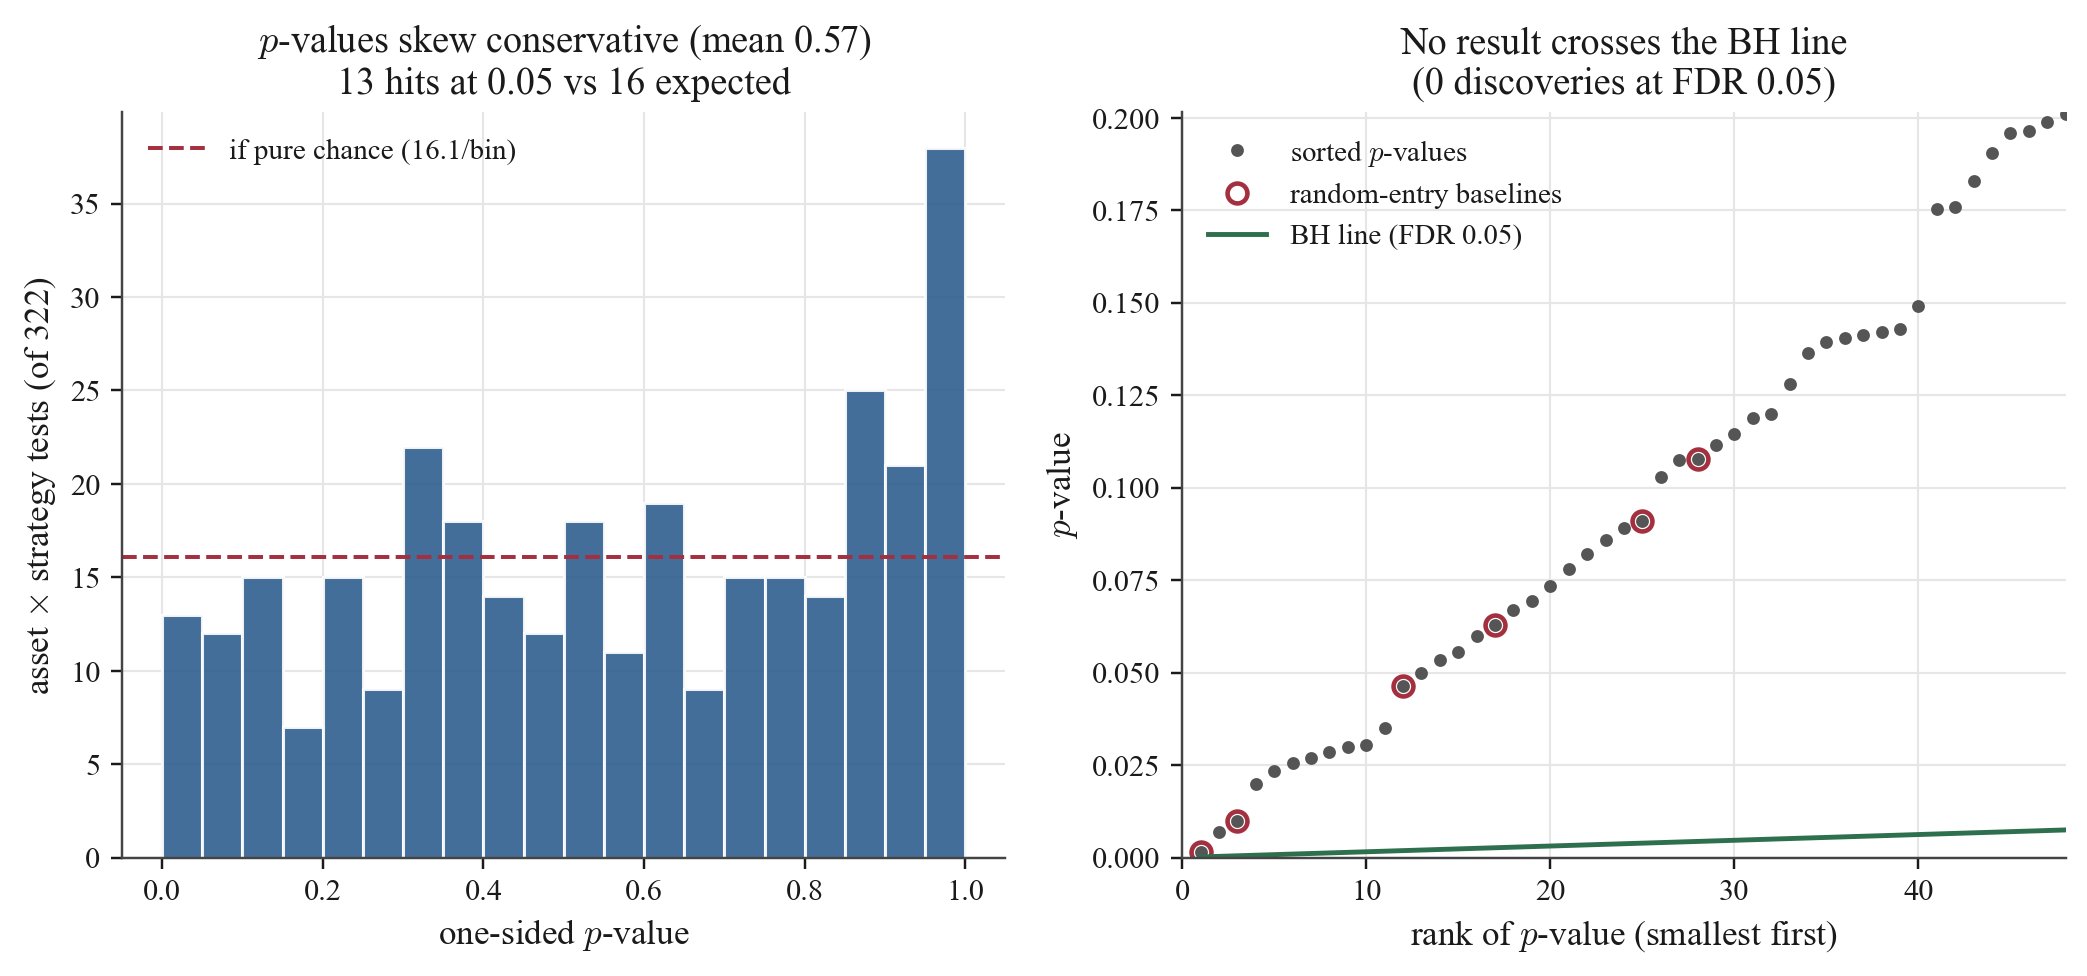
\includegraphics[width=0.95\textwidth]{cross_asset_multiplicity.png}
\caption{Cross-asset panel of $322$ structure-preserving tests across $47$ instruments. Left: the $p$-value histogram skews conservative, with $13$ nominal rejections versus $16.1$ expected by chance. Right: the Benjamini--Hochberg plot---no ordered $p$-value crosses the FDR line, so there are zero discoveries; circled points are random-entry baselines, which sit among the smallest $p$-values.}
\label{fig:cross_asset}
\end{figure}

\paragraph{What the panel is, and is not.} Three selection questions deserve direct answers. First, on \emph{strategy choice}: the eleven-rule panel is fixed, with thresholds set ex ante (\ref{app:strategy_rules}) and applied identically to every asset; there is no per-asset re-optimization, so the within-scan researcher degrees of freedom are confined to the asset universe rather than the rules. Second, on \emph{asset choice}: the $47$ instruments are those for which a completed structure-preserving run existed---an availability sample spanning equity ETFs, single names, futures, commodities, FX, and crypto, not a set curated on outcomes. We report every test that exists rather than a selected subset, and the embedded random-entry baselines act as a built-in negative control: any selection or specification artifact that inflated significance would inflate the baselines too, and it does not. Third, on \emph{survivorship}: the universe contains currently traded instruments, so delisted names are absent. This cannot manufacture the finding, for two reasons. The result is a \emph{null}, and survivorship would if anything bias toward detecting skill (survivors trend upward); and the structure-preserving null absorbs that drift by construction, since it reprices the same trades on the same surviving path. The honest characterization is therefore a pooled, dependence-laden convenience sample---correlated assets and shared strategy logic---analyzed with dependence-aware multiplicity control \cite{benjaminihochberg1995,BenjaminiYekutieli2001}, not a designed-universe study; we present it as breadth evidence against the existence of broad, easily found timing skill, not as a representative census.

\subsection{Frequency robustness check}
\label{sec:frequency-robustness}

The daily-only criticism is addressed with a bounded frequency-robustness check. The same walk-forward engine is run on SPY, QQQ, and BTC-USD at three bar intervals: daily, 4-hour, and hourly. To keep the comparison aligned with the shorter Yahoo Finance intraday history window, each interval uses at most the four most recent non-overlapping test folds per ticker. The test windows are scaled to roughly the same calendar length: 126 daily bars, 252 four-hour bars, and 882 hourly bars. Each retained strategy-fold panel must contain at least five trades and is evaluated with $M=1{,}000$ structure-preserving null simulations and one outer run (Table~\ref{tab:frequency_robustness}).

\begin{table}[H]
\centering
\caption{Bounded frequency-robustness summary across SPY, QQQ, and BTC-USD.}
\label{tab:frequency_robustness}
{\small
\renewcommand{\arraystretch}{1.12}
\begin{adjustbox}{max width=\textwidth}
\begin{tabular}{@{}lrrrrrrl@{}}
\toprule
Interval & Strategies & Panels & Bars/fold & Min mean $p$ & Best percentile & Mean sig.\ panels & Best-percentile strategy \\
\midrule
Daily   & 6 & 18 & 126 & 0.244 & 75.7 & 0.0\% & Turn-of-Month \\
4-hour  & 5 & 10 & 252 & 0.593 & 40.8 & 0.0\% & Oversold Reversion \\
Hourly  & 5 & 15 & 882 & 0.236 & 76.5 & 4.0\% & Oversold Reversion \\
\bottomrule
\end{tabular}
\end{adjustbox}
}
\par\vspace{0.5em}
\begin{minipage}{0.95\textwidth}
\centering
\footnotesize\emph{Notes.} The panel uses the three tickers common to the daily, 4-hour, and hourly runs. ``Strategies'' counts strategies with at least one retained panel at that interval. ``Mean sig.\ panels'' averages the per-strategy share of retained panels with $p\le0.05$. The run is exploratory: one outer run, recent folds only, and sparse retained panels at higher frequencies.
\end{minipage}
\end{table}

\begin{figure}[htbp]
\centering
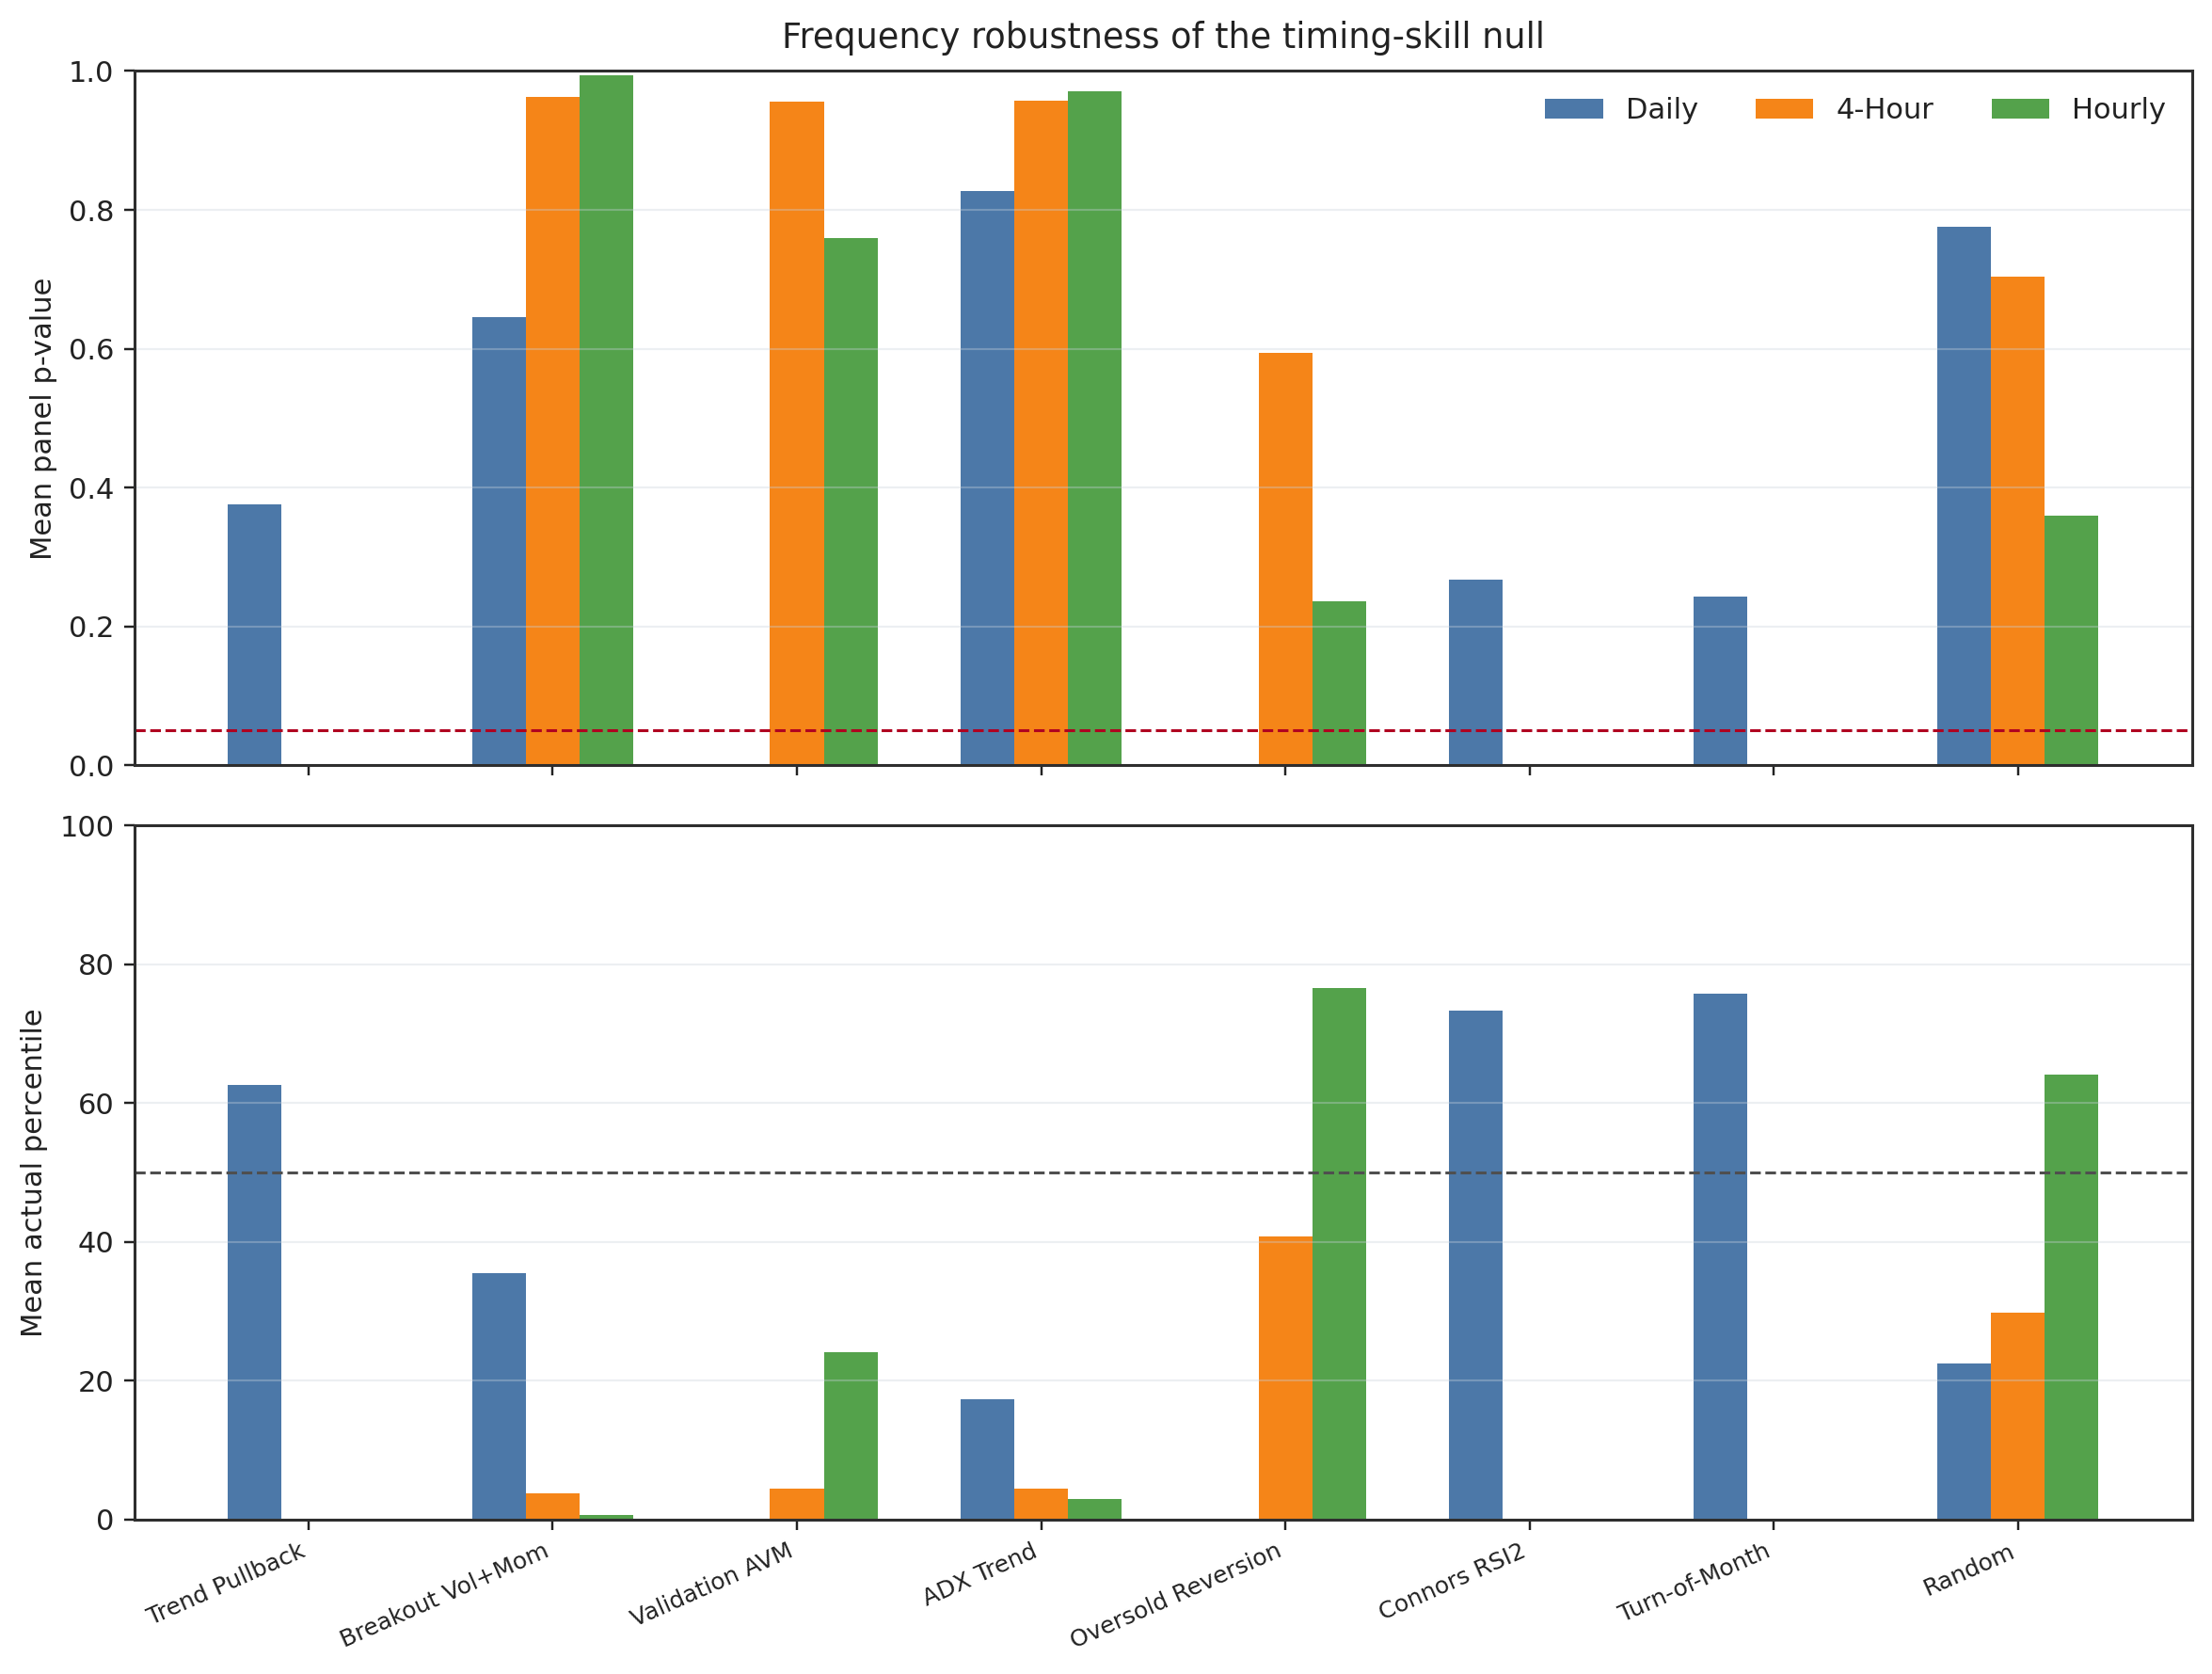
\includegraphics[width=0.95\textwidth]{frequency_robustness_pvalue_percentile.png}
\caption{Frequency-robustness check across recent daily, 4-hour, and hourly panels. The top panel reports mean panel $p$-value by strategy and interval; the bottom panel reports mean actual percentile.}
\label{fig:frequency_robustness}
\end{figure}

The frequency check does not overturn the main result, but with at most five retained panels per interval it is underpowered to do so (Figure~\ref{fig:frequency_robustness}). The 4-hour panel is uniformly weak, with no retained strategy averaging above the null median and a best mean $p$-value of 0.593. The hourly panel contains one favorable mean-reversion result: Oversold Reversion averages percentile 76.5 with mean $p=0.236$ and one significant panel among five retained panels. That evidence is positive but not decisive, especially because the Random baseline also looks favorable on this small hourly slice. The right interpretation is therefore modest: shortening the bar interval does not reveal broad, stable entry-placement skill, but the sparse hourly panel motivates a larger seed-robust intraday study.

\subsection{The profit--skill divergence}

The central finding is the systematic divergence between profitability and entry-placement evidence. Of the ten strategies with positive cumulative returns, only four show even weak evidence of favorable entry placement. The remaining six are profitable but statistically indistinguishable from random timing under the structure-preserving null. The explanation is direct: gold futures appreciated over the sample period (buy-and-hold return of $14.670$), so any long-biased strategy with sufficient exposure will capture some of that appreciation regardless of when it enters. The structure-preserving null absorbs this drift because it randomizes entries on the same appreciating price path, exposing how much of the realized return comes from entry placement versus the asset's secular trend.

This divergence has implications for overfitting. A researcher who evaluates candidates by cumulative return alone will preferentially select strategies whose structural features (holding period, trade frequency, direction bias) interact favorably with the realized path. The structure-preserving null provides a correction: it asks whether the selected entry placement is better than what a randomly timed strategy with the same structural features would have achieved. When the answer is no, the apparent ``edge'' is better explained by structural exposure to a trending asset than by entry placement.

\subsection{The random baseline as a diagnostic}

The random baseline provides the clearest illustration of why profitability is insufficient for inference. The Random strategy generates entries with probability 0.07 per bar, ignores all market features, and holds positions for randomly drawn durations. It is profitable at $0.601$, a cumulative return that exceeds nine of the ten rule-based strategies (all except ADX Trend at $0.803$). Yet it classifies as Below null median with $p=0.710$ and percentile $29.0$. Its RCSI robustness is $-0.103 \pm 0.523$, reflecting both inferior timing and extreme instability across seeds.

This result is expected under the framework. The Random strategy's profitability derives from long-biased exposure to an appreciating asset rather than from any market signal. Its timing, being random, should sit near the center of its own null distribution across repeated seeds; the seed-42 realization happens to fall below the median. The result illustrates the premise that profit alone does not identify skill: a strategy with no timing information can produce substantial returns, yet the structure-preserving null classifies its entry placement as statistically ordinary relative to randomized placement with the same structural burden.

\subsection{Anatomy of weak skill}

Four strategies classify as weak skill: Squeeze Breakout ($p=0.053$, percentile $94.7$), ADX Trend ($p=0.141$, percentile $85.9$), Connors RSI2 ($p=0.143$, percentile $85.7$), and Breakout Vol+Mom ($p=0.176$, percentile $82.4$). These share two common traits.

First, all four embed explicit regime or volatility filters that restrict entries to structurally favorable environments. Squeeze Breakout requires volatility compression before entering. ADX Trend requires confirmed directional strength. Connors RSI2 requires extreme short-term oversold conditions. Breakout Vol+Mom requires both participation and momentum confirmation. These filters function as implicit timing mechanisms by concentrating entries in periods where subsequent returns have been above average. Second, all four show stable percentile placements across robustness seeds, with standard deviations of $0.3$ to $0.5$ percentage points. Their weak-skill classifications are not artifacts of a particular simulation draw.

The common thread is that these strategies incorporate the most informative conditioning variables. The filters do not guarantee strong timing (none crosses $p \le 0.05$), but they concentrate entries in a way that modestly outperforms random placement. The strategies classified as Random or luck, by contrast, use broader or less discriminating entry conditions. Turn-of-Month relies on a simple calendar rule. Donchian Reentry uses a breakout-only filter. These broader conditions dilute any conditional timing advantage. Specificity in entry conditions, not complexity, is the mechanism through which weak timing advantages emerge.

\subsection{Per-strategy Monte Carlo distribution summaries}

Each Monte Carlo distribution figure reports the realized outcome, the null median, null 5th and 95th percentiles, and the derived $p$-value and percentile. Table \ref{tab:mc} compiles these verified caption values.

\clearpage
\begin{table}[p]
\centering
\caption{Monte Carlo distribution summaries per strategy (all values taken from the strategy-specific distribution captions, $M=5{,}000$).}
\label{tab:mc}
{\small
\renewcommand{\arraystretch}{1.15}
\setlength{\tabcolsep}{6pt}
\begin{adjustbox}{max width=\textwidth}
\begin{tabular}{@{}lrrrrrr@{}}
\toprule
Strategy & Actual & Null median & Null 5th & Null 95th & $p$-value & Percentile \\
\midrule
Trend Pullback      & 0.0832 & 0.4013 & -0.0611 & 1.0725 & 0.8700 & 13.0 \\
Breakout Vol+Mom    & 0.2967 & 0.1285 & -0.1215 & 0.4419 & 0.1758 & 82.4 \\
Mean Rev Vol Filter & -0.0097 & 0.0199 & -0.0897 & 0.1436 & 0.662\phantom{0} & 33.8 \\
Validation AVM      & 0.2187 & 0.1429 & -0.1285 & 0.4919 & 0.3447 & 65.5 \\
ADX Trend           & 0.8032 & 0.3705 & -0.0928 & 1.0660 & 0.1414 & 85.9 \\
Oversold Reversion  & 0.0822 & 0.0464 & -0.1007 & 0.2126 & 0.3409 & 65.9 \\
Squeeze Breakout    & 0.0649 & 0.0107 & -0.0483 & 0.0655 & 0.0534 & 94.7 \\
Connors RSI2        & 0.1184 & 0.0216 & -0.1112 & 0.1736 & 0.1428 & 85.7 \\
Donchian Reentry    & 0.0713 & 0.1462 & -0.1328 & 0.5173 & 0.6469 & 35.3 \\
Turn-of-Month       & 0.3229 & 0.1553 & -0.1498 & 0.5794 & 0.2336 & 76.7 \\
Random              & 0.6011 & 0.9381 & \phantom{-}0.1276 & 2.3314 & 0.7103 & 29.0 \\
\bottomrule
\end{tabular}
\end{adjustbox}
}
\par\vspace{0.75em}
\begin{minipage}{0.95\textwidth}
\centering
\footnotesize\emph{Notes.} ``Null'' values summarize the structure-preserving Monte Carlo distribution for each strategy as displayed in the per-strategy distribution figures. Each caption reports transaction cost $c=0.000470$.
\end{minipage}
\end{table}
\clearpage

Table \ref{tab:mc} makes the inference problem concrete. For several strategies, the realized outcome sits well inside the null distribution, despite positive profit. Trend Pullback illustrates this clearly. Its return is 0.0832, while the null median is 0.4013 and the p-value is 0.8700. A profitability-only verdict would call this strategy successful. The structure-preserving null reveals that it underperforms random timing. Its realized entries are \emph{worse} than what chance would typically produce.

\section{Market regime analysis}

The regime figures are descriptive diagnostics, not separate hypothesis tests. They summarize trade-level performance using a trade-level return ratio defined as mean return divided by standard deviation, a Sharpe-like ratio per trade rather than an annualized Sharpe. The regime heatmap (Figure~\ref{fig:regime_heatmap}) reports values and trade counts per regime, suppressing regime cells with fewer than five trades. The heatmap reports 11 suppressed cells. Because many regime cells remain small even after suppression, the regime section is used to generate hypotheses about conditional behavior rather than to establish regime-specific timing skill.

Table \ref{tab:regimes} reproduces the verified regime values shown in the heatmap. Cells not shown in the heatmap are marked as suppressed.

\begin{table}[htbp]
\centering
\caption{Regime-level trade performance (trade-level return ratio) taken from the regime heatmap. Values are shown as ratio with trade count in parentheses.}
\label{tab:regimes}
\small
\renewcommand{\arraystretch}{1.1}
\begin{tabular}{lccc}
\toprule
Strategy & Calm & Neutral & Stressed \\
\midrule
Trend Pullback      & 0.02 (n=10) & 0.13 (n=25) & 0.03 (n=42) \\
Breakout Vol+Mom    & 0.22 (n=14) & 0.14 (n=24) & 0.29 (n=8) \\
Mean Rev Vol Filter & -0.26 (n=10) & suppressed & suppressed \\
Validation AVM      & 0.34 (n=13) & 0.15 (n=22) & suppressed \\
ADX Trend           & 0.16 (n=50) & 0.27 (n=60) & suppressed \\
Oversold Reversion  & 0.29 (n=18) & 0.18 (n=12) & suppressed \\
Squeeze Breakout    & suppressed & suppressed & suppressed \\
Connors RSI2        & 0.17 (n=18) & 0.30 (n=23) & suppressed \\
Donchian Reentry    & 0.02 (n=28) & 0.08 (n=32) & suppressed \\
Turn-of-Month       & 0.10 (n=80) & 0.21 (n=61) & suppressed \\
Random              & 0.01 (n=76) & 0.11 (n=66) & 0.14 (n=73) \\
\bottomrule
\end{tabular}
\end{table}

Three regime patterns emerge, each with implications for the timing-skill interpretation.

First, several strategies show their strongest trade-level ratios in Neutral regimes. ADX Trend reaches 0.27 (n=60) in Neutral versus 0.16 (n=50) in Calm, and Connors RSI2 reaches 0.30 (n=23) in Neutral versus 0.17 (n=18) in Calm. This pattern suggests that timing skill, to the extent it exists, concentrates in moderate-volatility environments where trends are identifiable but not disrupted by extreme price action. Neutral regimes offer a favorable signal-to-noise ratio: volatility is sufficient to generate meaningful moves but not so extreme as to overwhelm technical signals.

Second, Breakout Vol+Mom is the only strategy with strong Stressed-regime performance at 0.29 (n=8) in the regime heatmap (Figure~\ref{fig:regime_heatmap}); with only eight trades this cell is hypothesis-generating rather than confirmatory, and regime cells below roughly twenty trades should be read the same way. The result is consistent with the strategy's design: its volume and momentum filters select Stressed-period entries where a genuine breakout occurs rather than a false signal. The suppression of most Stressed-regime cells across the panel (contributing to the 11 suppressed cells) reveals that most strategies either avoid Stressed periods through explicit regime filters or generate too few trades in those periods to evaluate. This systematic avoidance is informative. The regime filters embedded in many strategies function as implicit timing mechanisms that concentrate trades in calmer environments, which explains part of their weak timing advantage.

Third, the Random baseline serves as a control. Its trade-level ratios are low but positive across all three regimes: 0.01 (n=76) in Calm, 0.11 (n=66) in Neutral, and 0.14 (n=73) in Stressed, with roughly even trade counts. This confirms that long-biased random exposure generates positive per-trade returns in all environments when the underlying asset appreciates. Profitability alone does not distinguish skill from drift. Rule-based strategies show \emph{higher} ratios in specific regimes while the random baseline is uniformly mediocre, suggesting that the timing advantage is regime-conditional rather than universal.

\section{Robustness across Monte Carlo seeds}

Seed robustness matters because a single simulation run produces a single null distribution, and the resulting $p$-value and percentile are themselves random variables that depend on the pseudo-random seed. If a strategy's classification changes across seeds, the single-run verdict is unreliable. The robustness design addresses this by evaluating each strategy under 100 independent outer runs, each with 5{,}000 simulations per run and transaction cost 0.000470, producing a distribution of skill metrics rather than a single point estimate.

\subsection{RCSI stability}

The RCSI robustness chart reports mean $\pm$ SD across seeds. Deterministic strategies show small dispersions. Trend Pullback reports $-0.361 \pm 0.005$ and ADX Trend reports $0.387 \pm 0.005$. These intervals confirm that, for deterministic strategies, the null distribution is stable across seeds and the RCSI is a reliable point estimate of timing quality. Random shows high variability at $-0.103 \pm 0.523$, consistent with the strategy being stochastic under outer-run variation: both the realized trade sequence and the null distribution change across seeds, producing compounding instability.

\subsection{Percentile stability}

The percentile robustness chart (Figure~\ref{fig:pct_robust}) reports mean $\pm$ SD percentile across seeds. Squeeze Breakout reports $94.3 \pm 0.3$, ADX Trend reports $86.2 \pm 0.4$, and Breakout Vol+Mom reports $82.7 \pm 0.5$. Random reports $48.3 \pm 25.6$, consistent with extreme instability across seeds.

These robustness results support three claims. First, the weak-skill classifications for Squeeze Breakout, ADX Trend, Connors RSI2, and Breakout Vol+Mom are stable. Their percentile placements vary by less than one percentage point across 100 seeds, showing that their relative positions in the null distribution are robust features of the data rather than artifacts of a particular simulation draw. Second, instability in the Random baseline's percentile ($\pm 25.6$) demonstrates that stochastic strategies require seed-level robustness analysis. A single-run percentile of 29.0 would have been 75 or 5 under a different seed, making any single-run verdict meaningless. Third, the contrast between stable weak-skill strategies and the unstable random baseline provides additional evidence that the weak-skill strategies contain some genuine timing information. Their consistency across seeds is itself a signal, because pure noise would produce the instability observed in the Random baseline.

\clearpage
\section{Figures}
\label{sec:figures-gallery}

The figures in this section are regenerated directly from the canonical trade logs and the structure-preserving null by \texttt{Code/regenerate\_gallery.py}, which reproduces the published Monte Carlo distribution statistics exactly (the script aborts on any material mismatch). They are not transcribed raster outputs.

\begin{figure}[htbp]
\centering
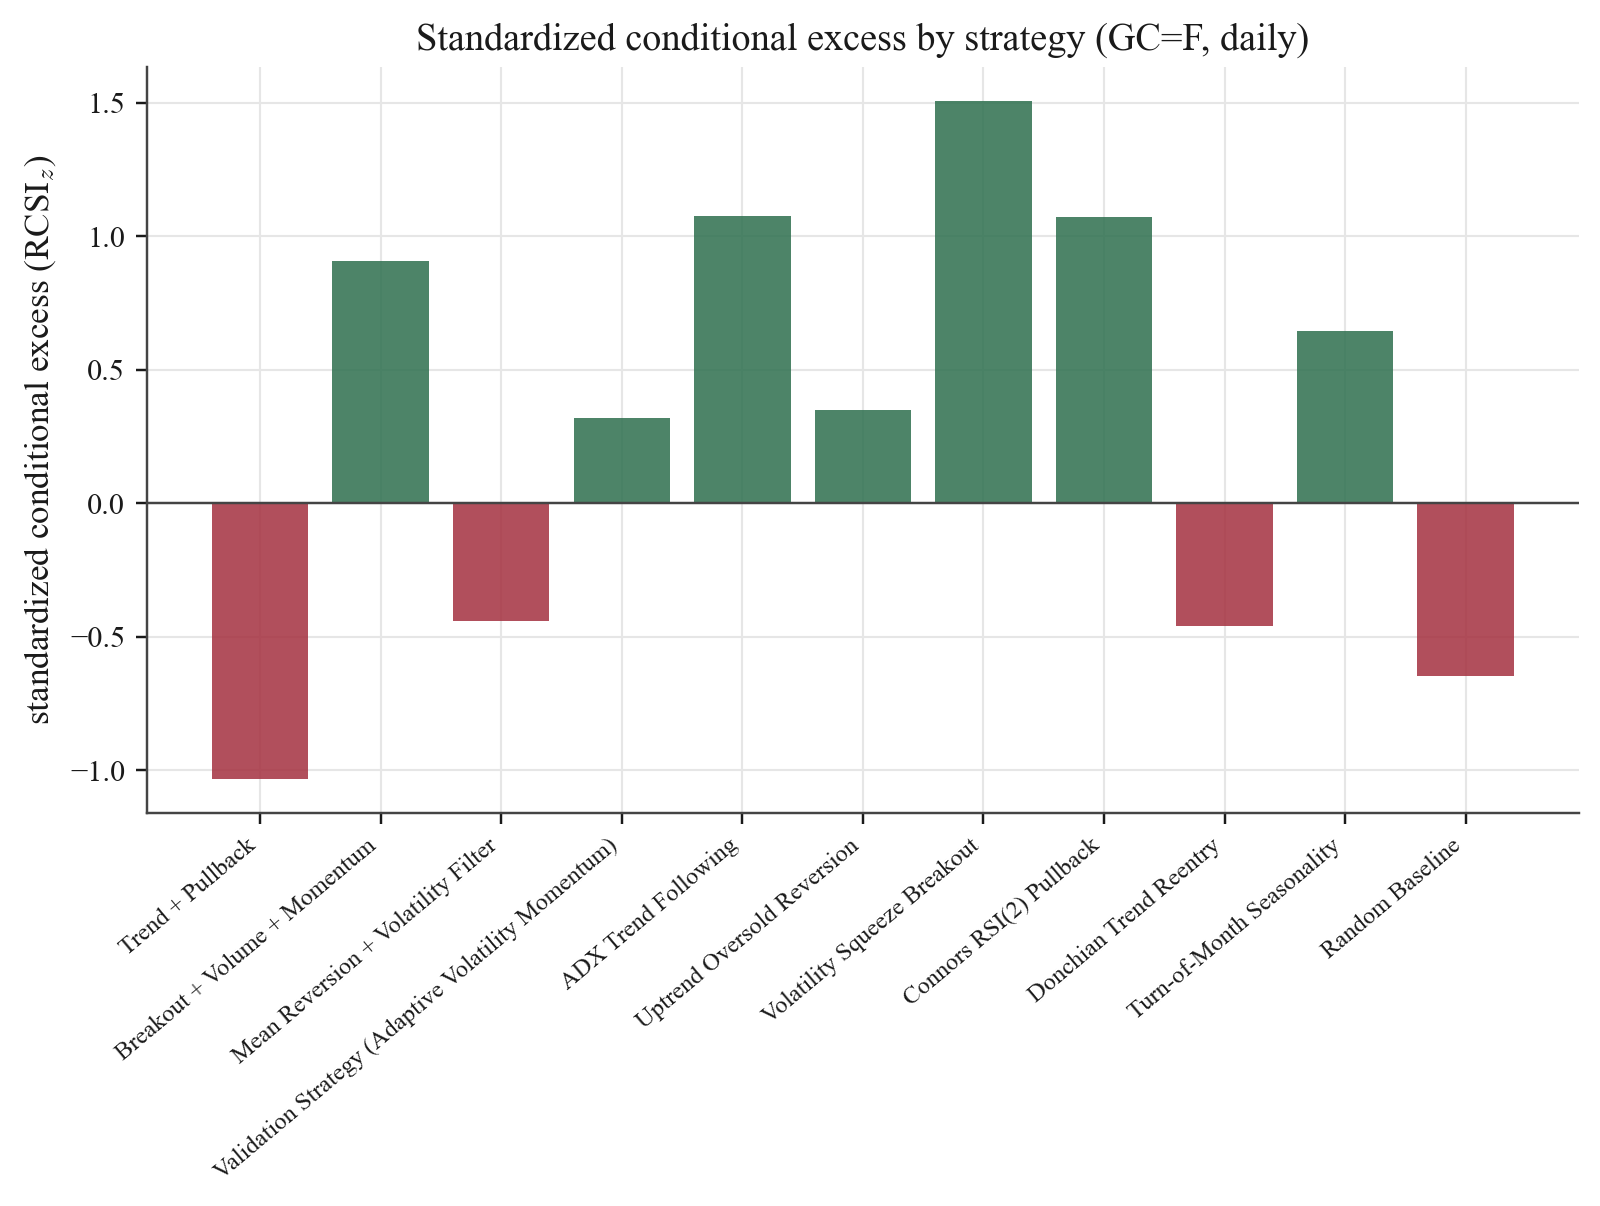
\includegraphics[width=0.85\textwidth]{rcsi_by_strategy.png}
\caption{GC=F. Relative Cumulative Skill Index (RCSI) by strategy (daily). The plot defines positive RCSI as performance above the strategy-specific Monte Carlo median, and uses RCSI along with $p$-value and percentile for classification.}
\label{fig:rcsi_by_strategy}
\end{figure}


\begin{figure}[htbp]
\centering
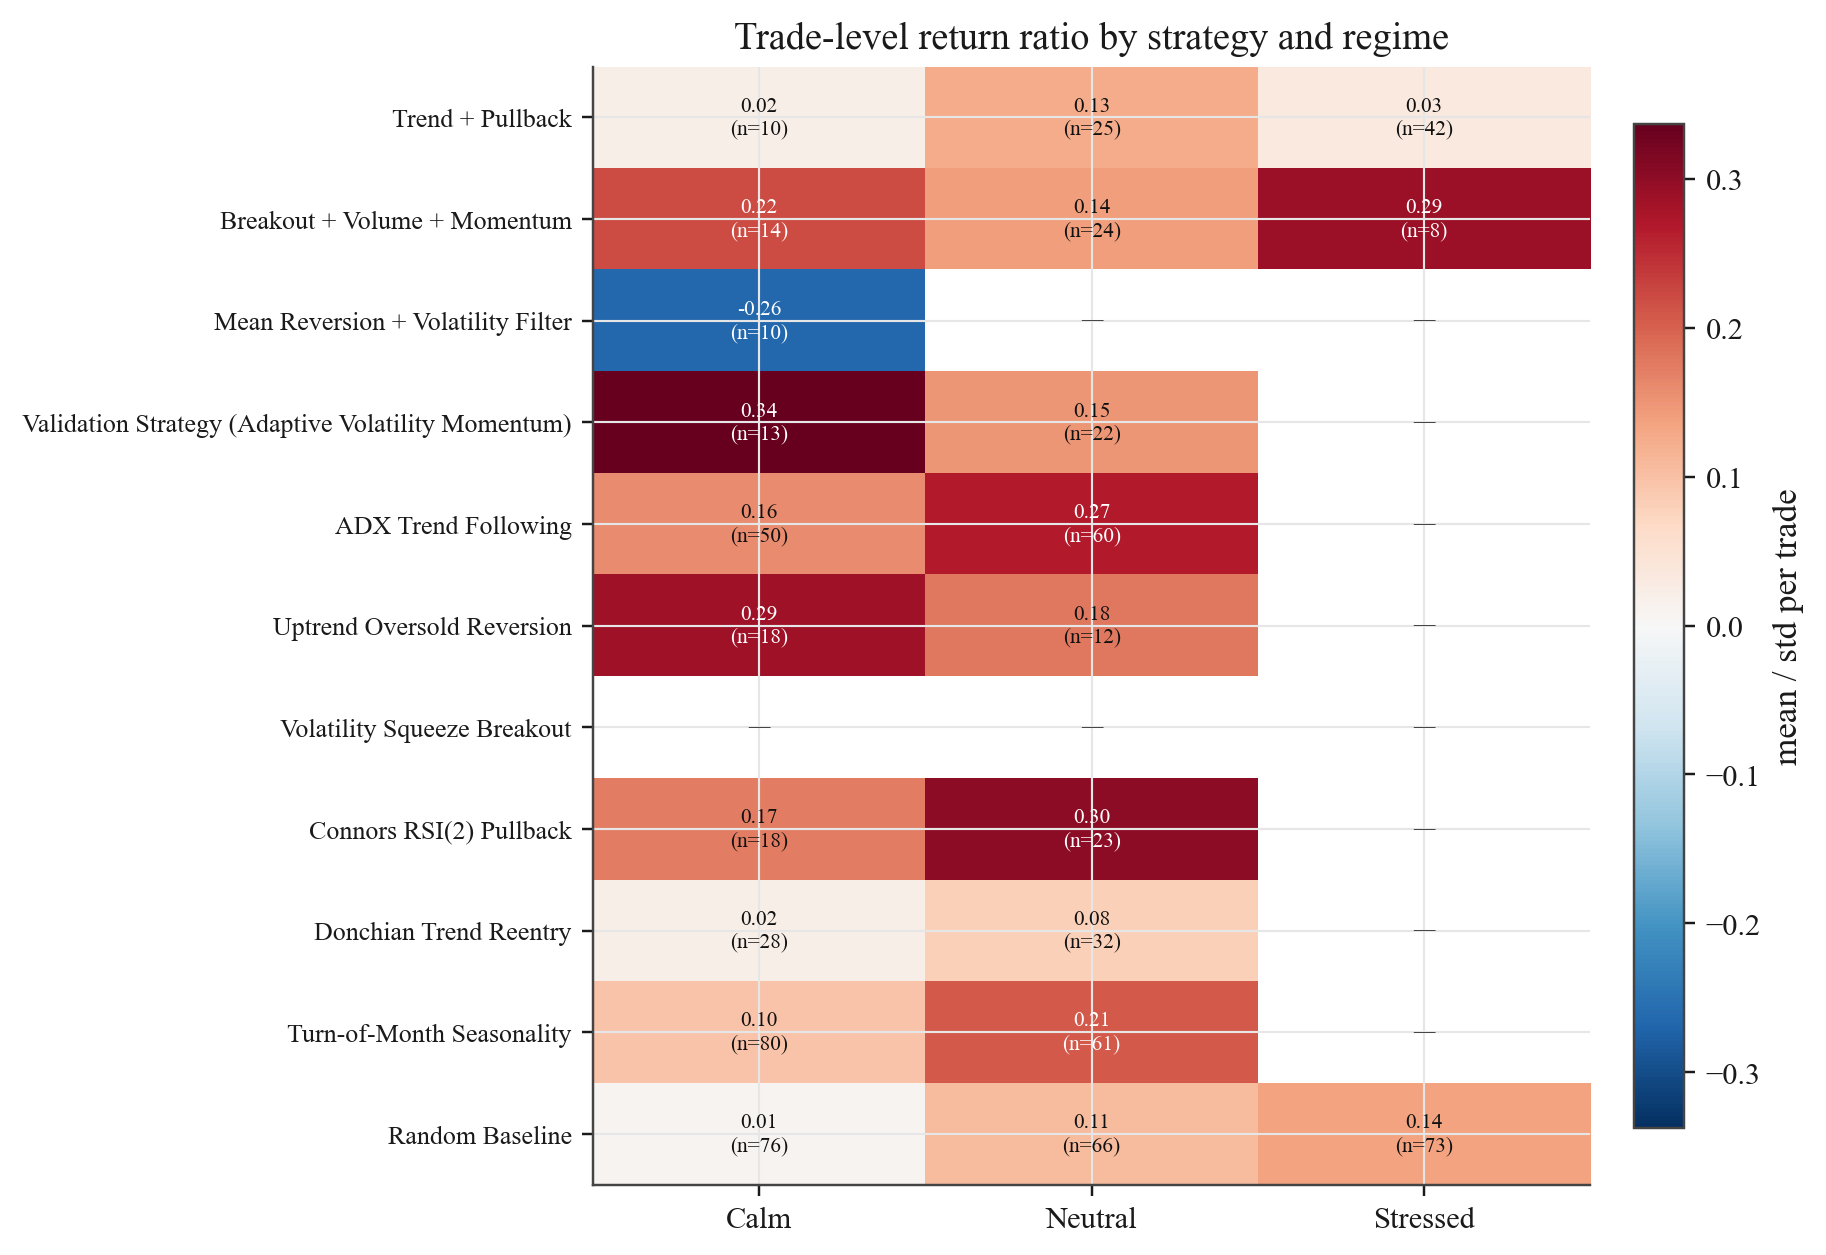
\includegraphics[width=0.66\textwidth]{regime_heatmap.png}
\caption{GC=F. Strategy performance across market regimes (daily). Cells show the trade-level return ratio and trade count: e.g., Breakout Vol+Mom is 0.22 (n=14) in Calm, 0.14 (n=24) in Neutral, and 0.29 (n=8) in Stressed. The figure reports ``Suppressed cells: 11'' for regimes with fewer than five trades.}
\label{fig:regime_heatmap}
\end{figure}

\begin{figure}[htbp]
\centering
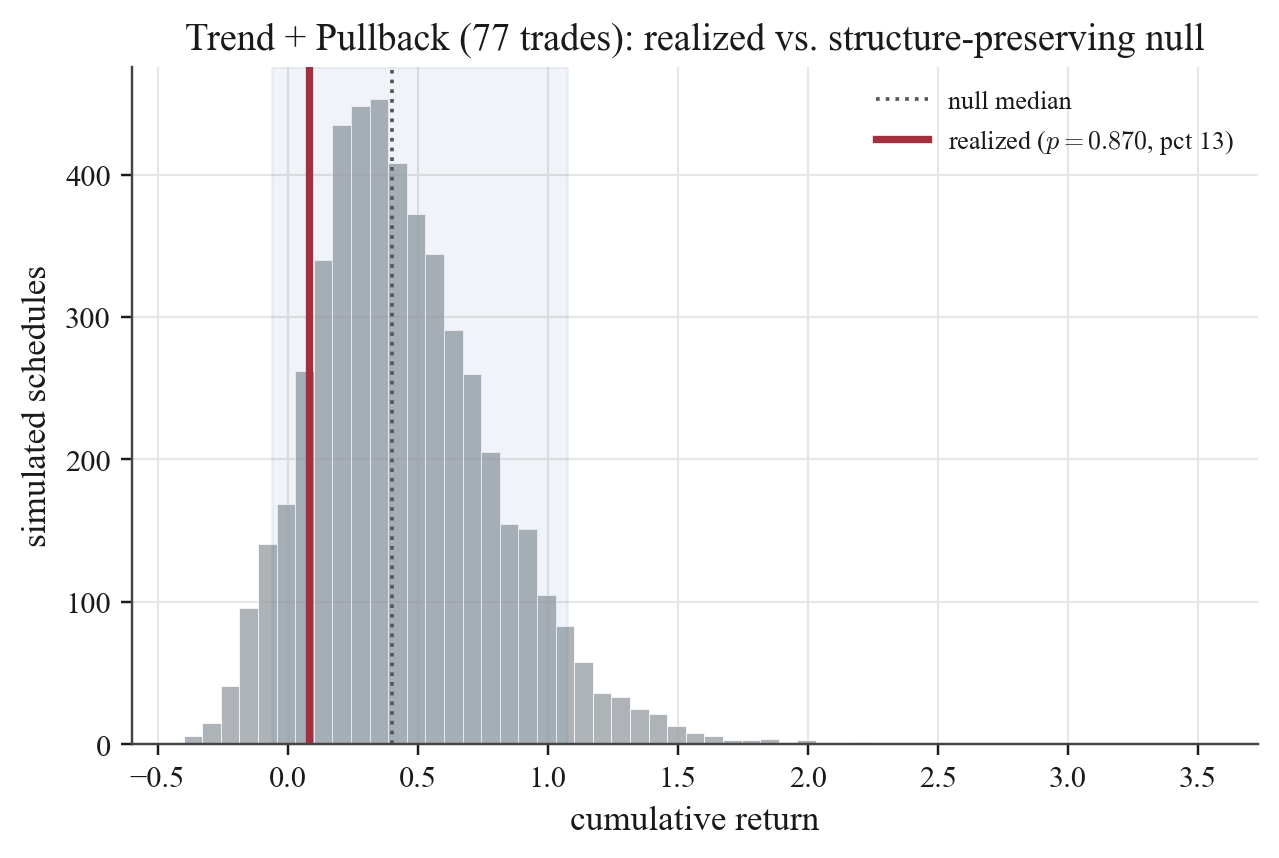
\includegraphics[width=0.72\textwidth]{mc_trend_pullback.png}
\caption{GC=F. Monte Carlo distribution of final returns, Trend Pullback (daily). Caption values: actual return = 0.0832; median simulated return = 0.4013; simulated 5th/95th = (-0.0611, 1.0725); p-value = 0.8700; actual percentile = 13.0; trades = 77; simulations = 5{,}000; transaction cost = 0.000470.}
\label{fig:mc_trend_pullback}
\end{figure}

\begin{figure}[htbp]
\centering
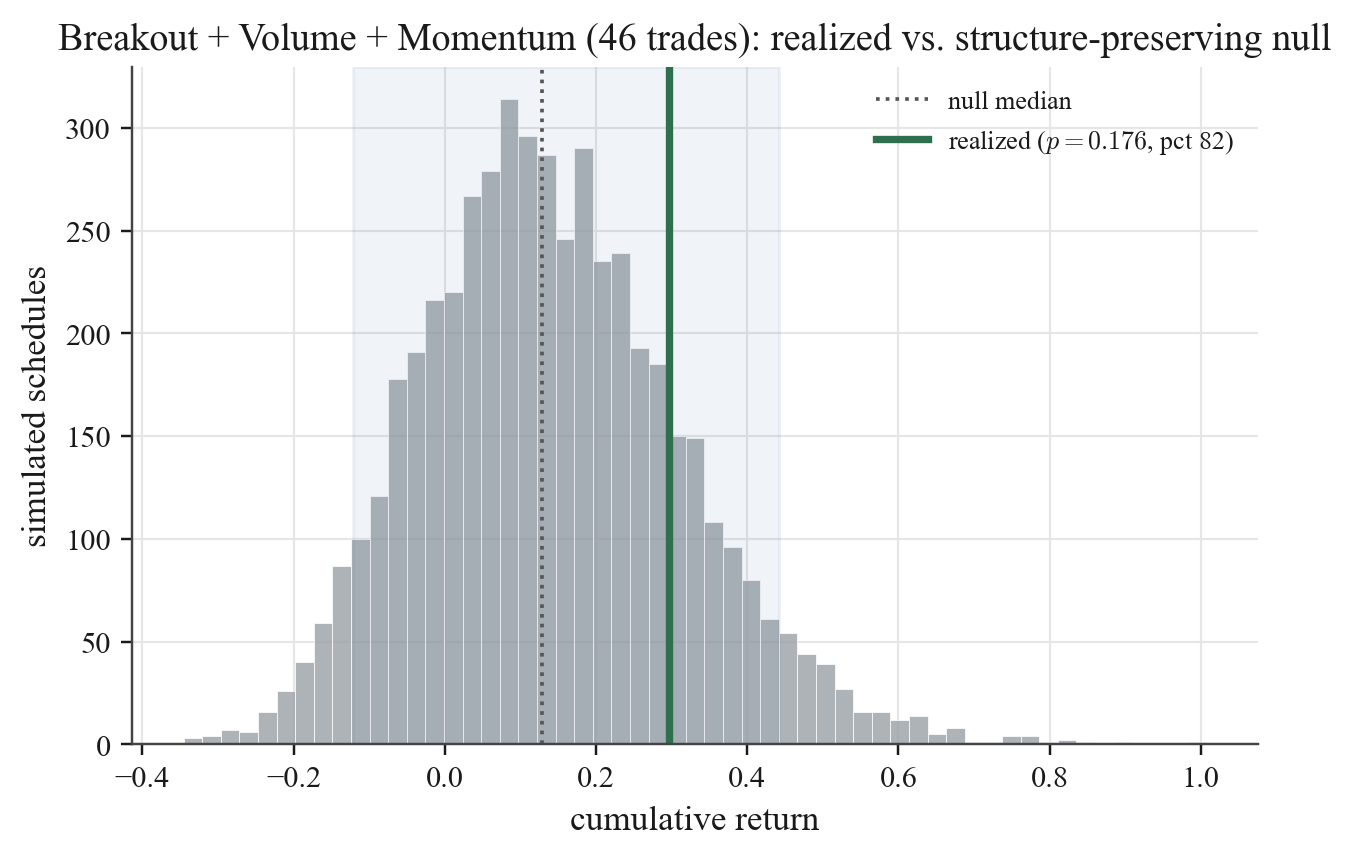
\includegraphics[width=0.72\textwidth]{mc_breakout_volume_momentum.png}
\caption{GC=F. Monte Carlo distribution of final returns, Breakout Vol+Mom (daily). Caption values: actual return = 0.2967; median simulated return = 0.1285; simulated 5th/95th = (-0.1215, 0.4419); p-value = 0.1758; actual percentile = 82.4; trades = 46; simulations = 5{,}000; transaction cost = 0.000470.}
\label{fig:mc_breakout}
\end{figure}

\begin{figure}[htbp]
\centering
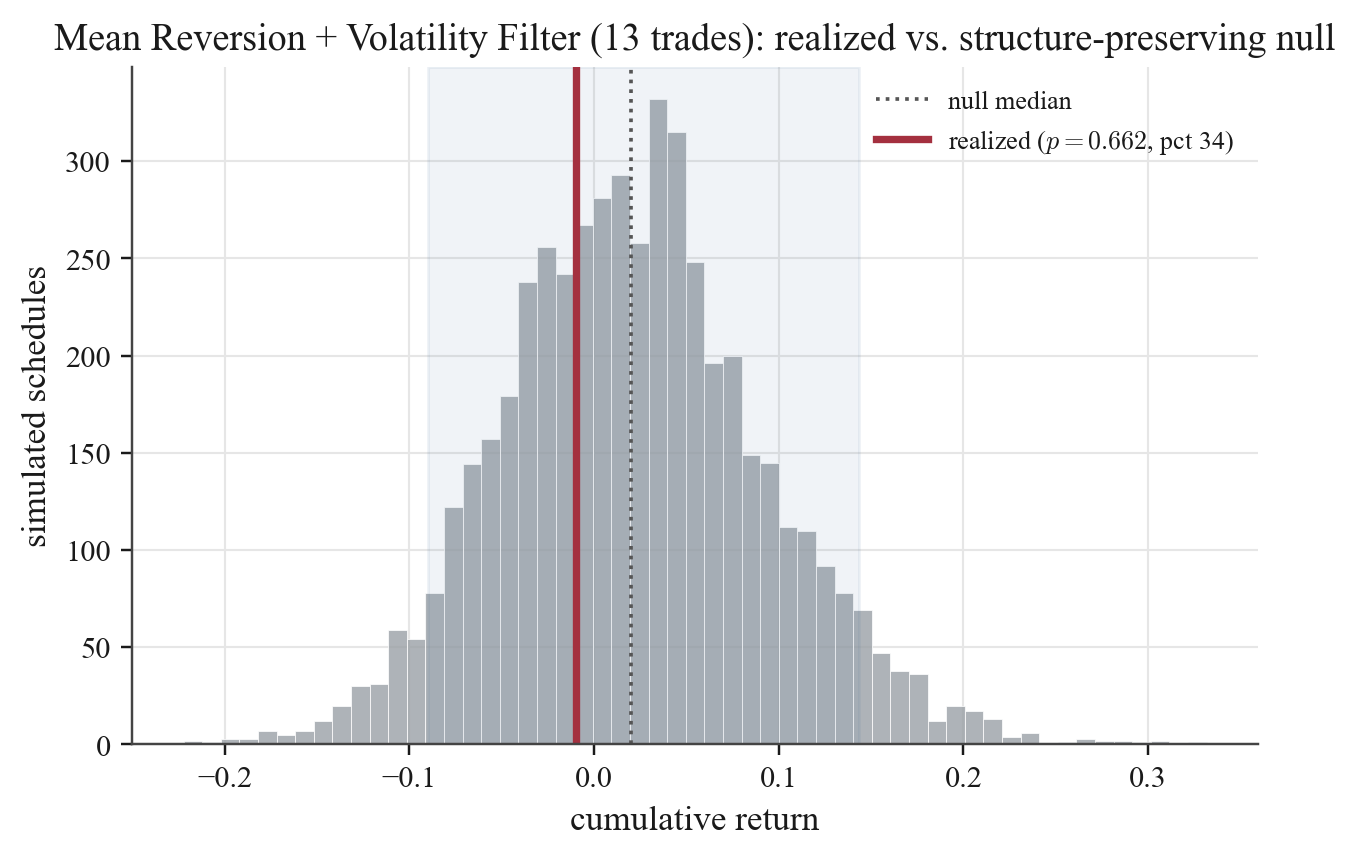
\includegraphics[width=0.72\textwidth]{mc_mean_reversion_vol_filter.png}
\caption{GC=F. Monte Carlo distribution of final returns, Mean Rev Vol Filter (daily). Caption values: actual return = -0.0097; median simulated return = 0.0199; simulated 5th/95th = (-0.0897, 0.1436); p-value = 0.662; actual percentile = 33.8; trades = 13; simulations = 5{,}000; transaction cost = 0.000470.}
\label{fig:mc_meanrev}
\end{figure}

\begin{figure}[htbp]
\centering
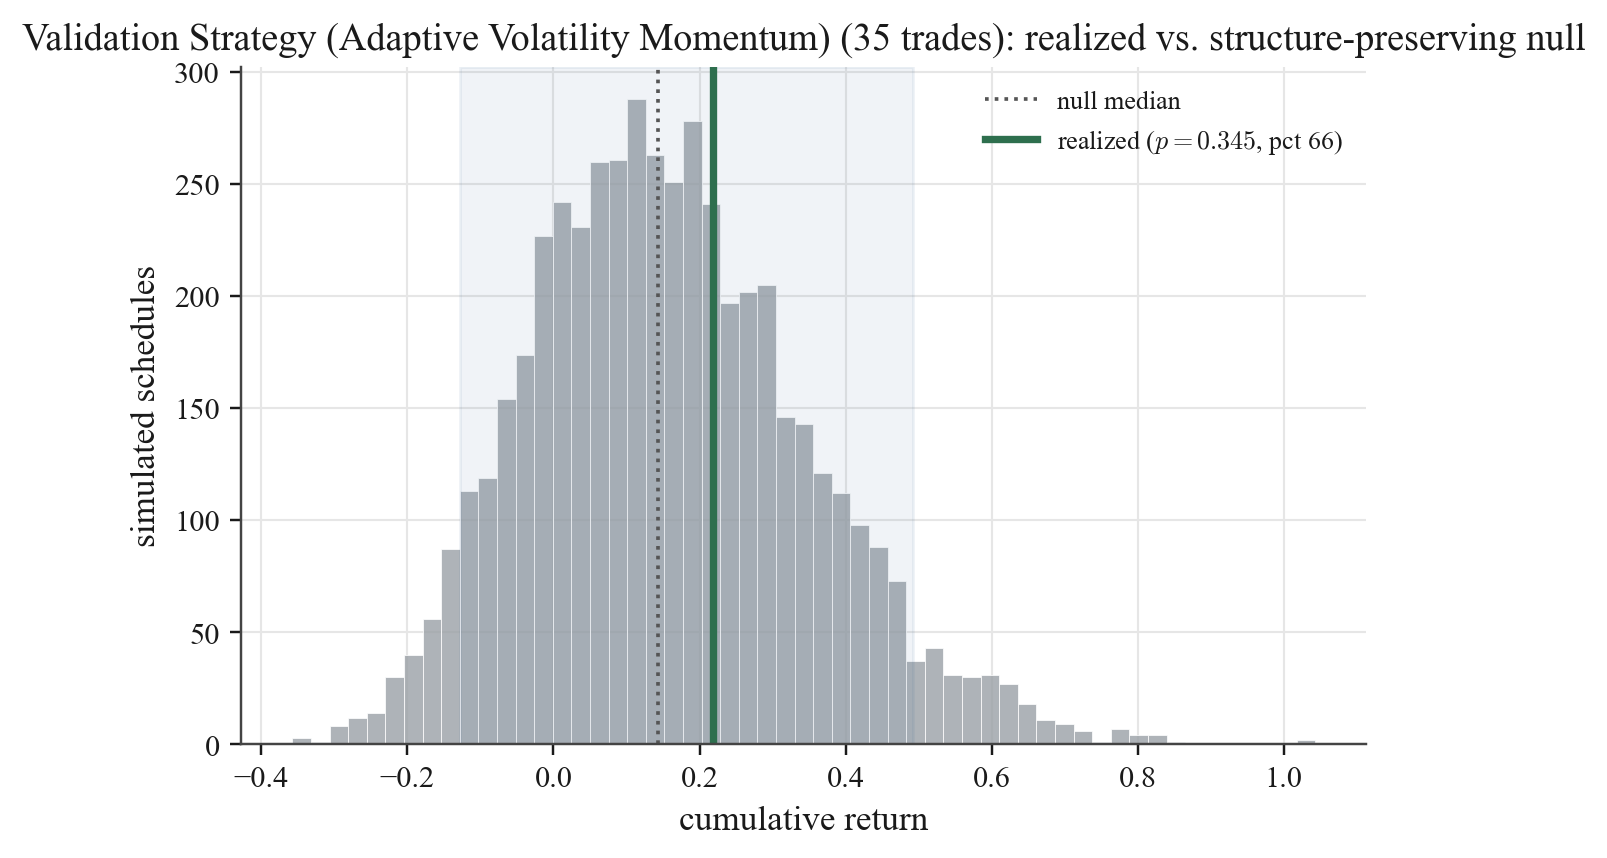
\includegraphics[width=0.72\textwidth]{mc_trend_momentum_verification.png}
\caption{GC=F. Monte Carlo distribution of final returns, Validation AVM (daily). Caption values: actual return = 0.2187; median simulated return = 0.1429; simulated 5th/95th = (-0.1285, 0.4919); p-value = 0.3447; actual percentile = 65.5; trades = 35; simulations = 5{,}000; transaction cost = 0.000470.}
\label{fig:mc_validation}
\end{figure}

\begin{figure}[htbp]
\centering
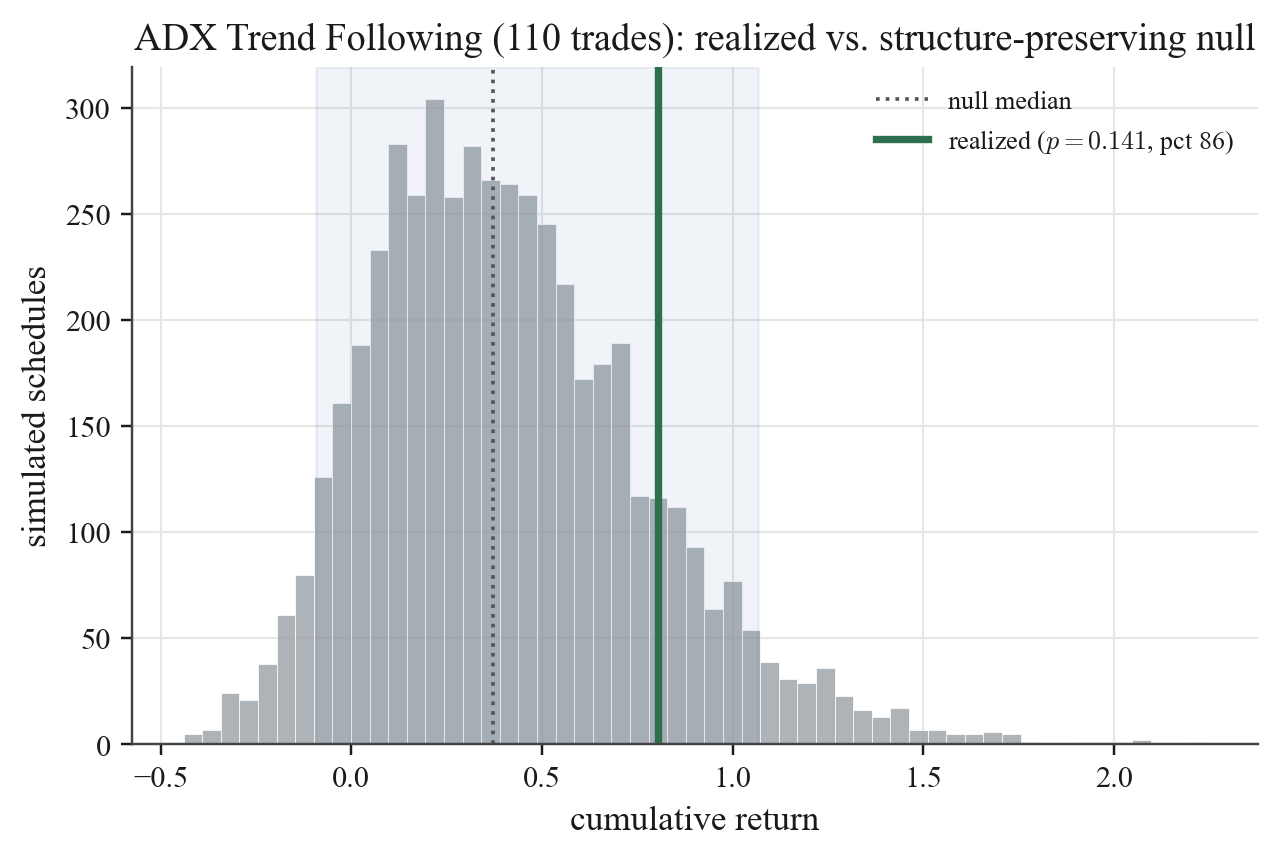
\includegraphics[width=0.72\textwidth]{mc_adx_trend_following.png}
\caption{GC=F. Monte Carlo distribution of final returns, ADX Trend (daily). Caption values: actual return = 0.8032; median simulated return = 0.3705; simulated 5th/95th = (-0.0928, 1.0660); p-value = 0.1414; actual percentile = 85.9; trades = 110; simulations = 5{,}000; transaction cost = 0.000470.}
\label{fig:mc_adx}
\end{figure}

\begin{figure}[htbp]
\centering
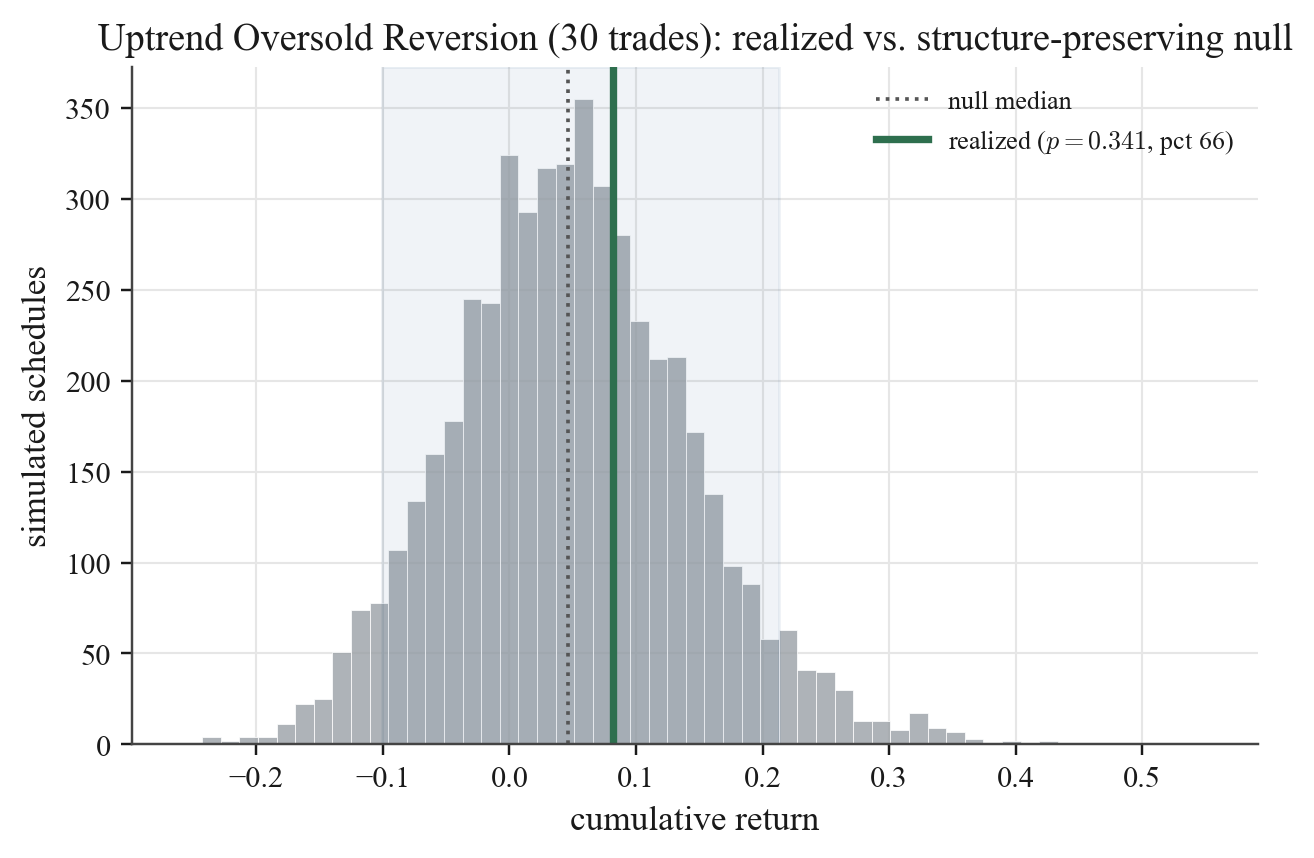
\includegraphics[width=0.72\textwidth]{mc_uptrend_oversold_reversion.png}
\caption{GC=F. Monte Carlo distribution of final returns, Oversold Reversion (daily). Caption values: actual return = 0.0822; median simulated return = 0.0464; simulated 5th/95th = (-0.1007, 0.2126); p-value = 0.3409; actual percentile = 65.9; trades = 30; simulations = 5{,}000; transaction cost = 0.000470.}
\label{fig:mc_oversold}
\end{figure}

\begin{figure}[htbp]
\centering
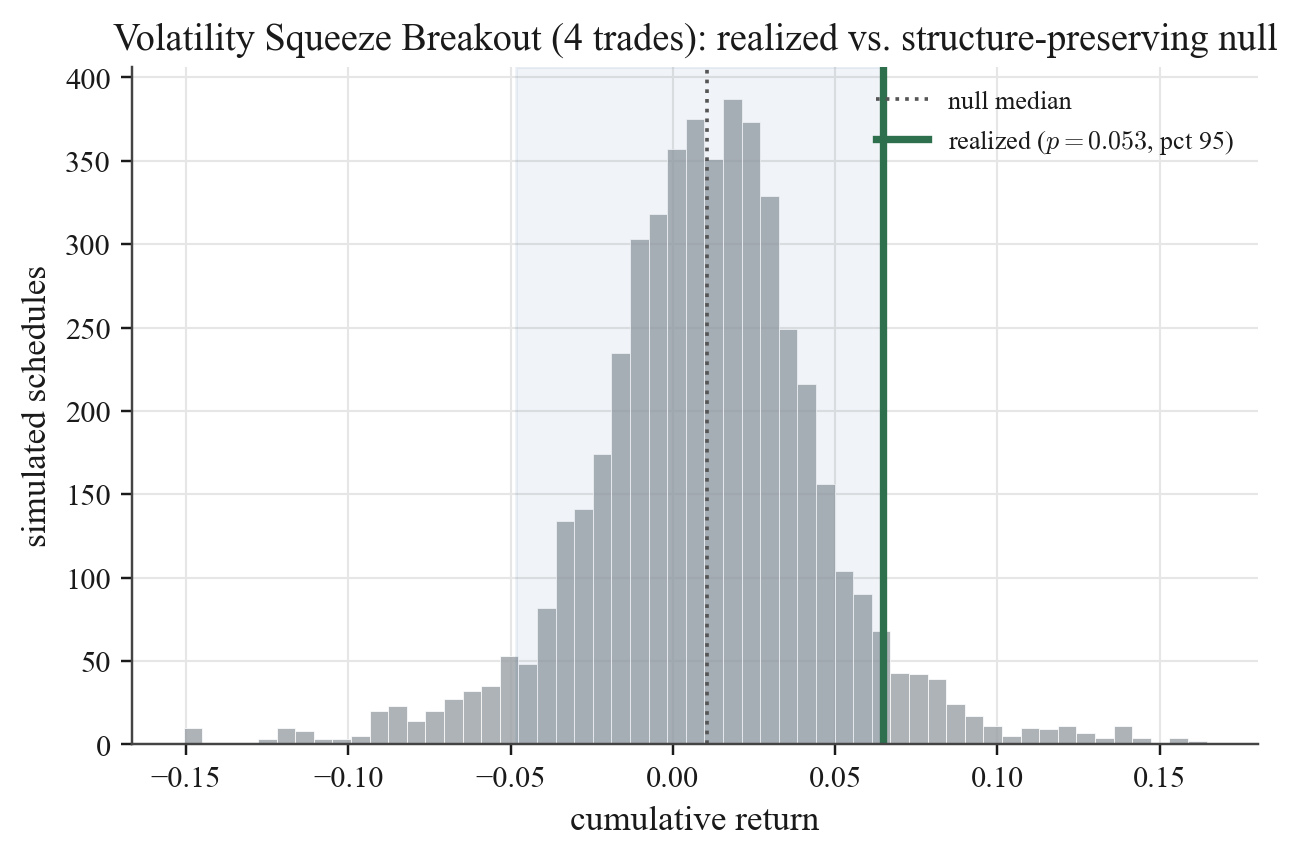
\includegraphics[width=0.72\textwidth]{mc_volatility_squeeze_breakout.png}
\caption{GC=F. Monte Carlo distribution of final returns, Squeeze Breakout (daily). Caption values: actual return = 0.0649; median simulated return = 0.0107; simulated 5th/95th = (-0.0483, 0.0655); p-value = 0.0534; actual percentile = 94.7; trades = 4; simulations = 5{,}000; transaction cost = 0.000470.}
\label{fig:mc_squeeze}
\end{figure}

\begin{figure}[htbp]
\centering
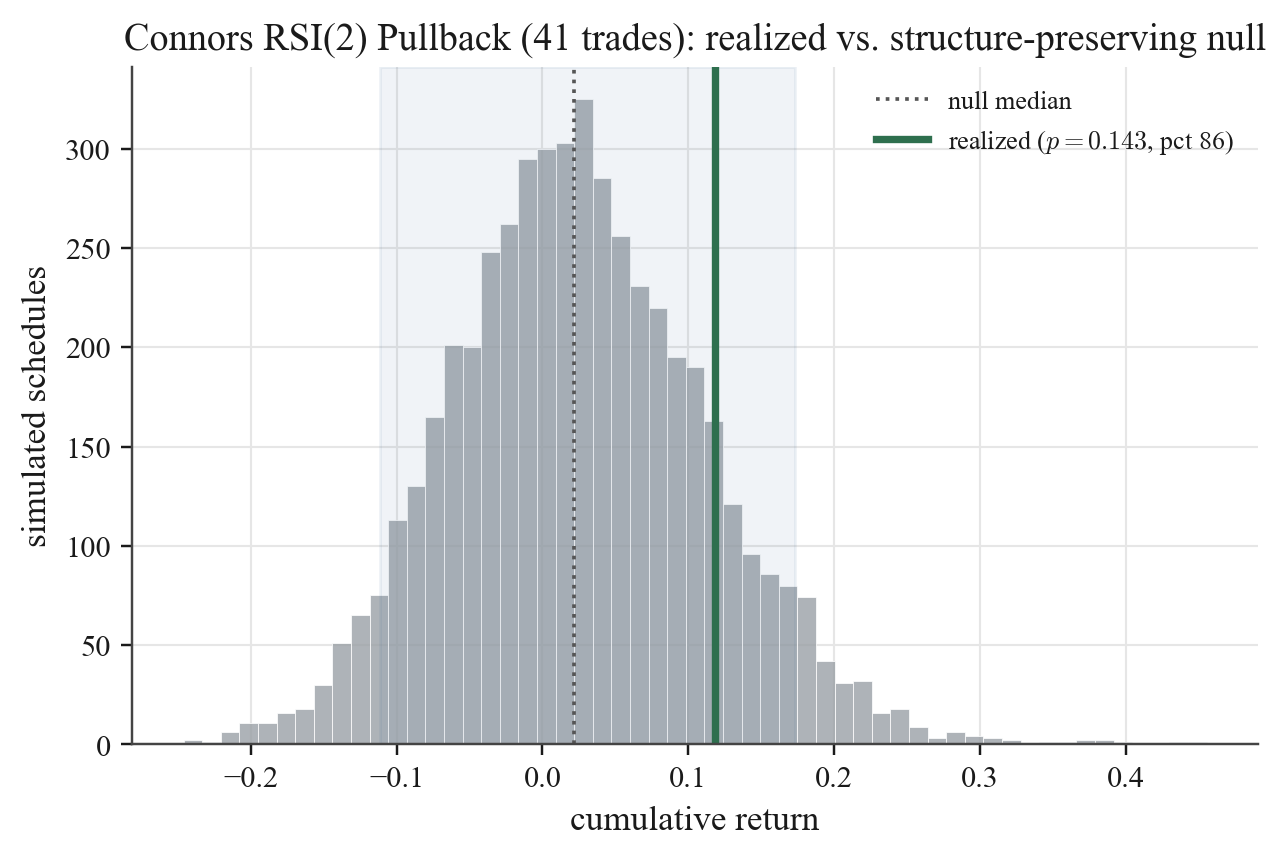
\includegraphics[width=0.72\textwidth]{mc_connors_rsi2_pullback.png}
\caption{GC=F. Monte Carlo distribution of final returns, Connors RSI2 (daily). Caption values: actual return = 0.1184; median simulated return = 0.0216; simulated 5th/95th = (-0.1112, 0.1736); p-value = 0.1428; actual percentile = 85.7; trades = 41; simulations = 5{,}000; transaction cost = 0.000470.}
\label{fig:mc_connors}
\end{figure}

\begin{figure}[htbp]
\centering
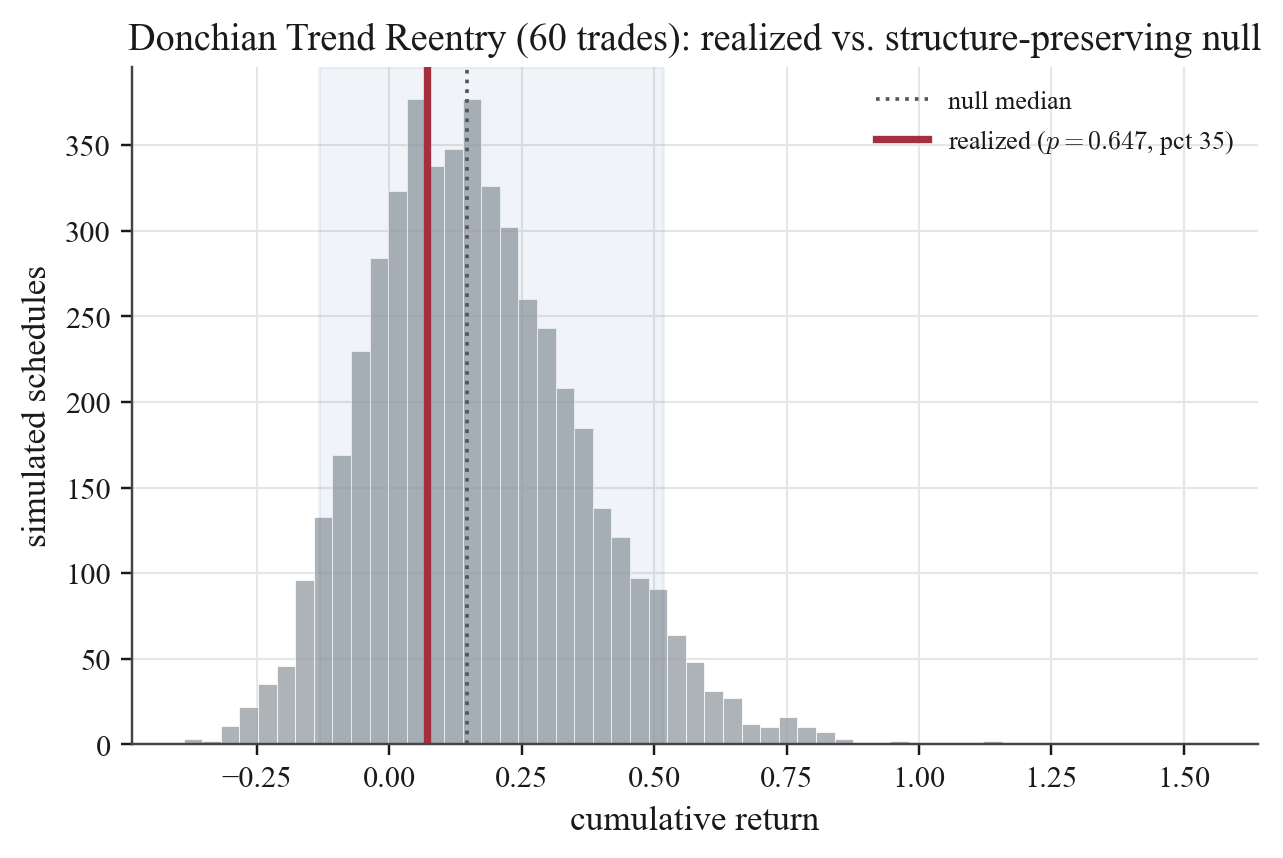
\includegraphics[width=0.72\textwidth]{mc_donchian_trend_reentry.png}
\caption{GC=F. Monte Carlo distribution of final returns, Donchian Reentry (daily). Caption values: actual return = 0.0713; median simulated return = 0.1462; simulated 5th/95th = (-0.1328, 0.5173); p-value = 0.6469; actual percentile = 35.3; trades = 60; simulations = 5{,}000; transaction cost = 0.000470.}
\label{fig:mc_donchian}
\end{figure}

\begin{figure}[htbp]
\centering
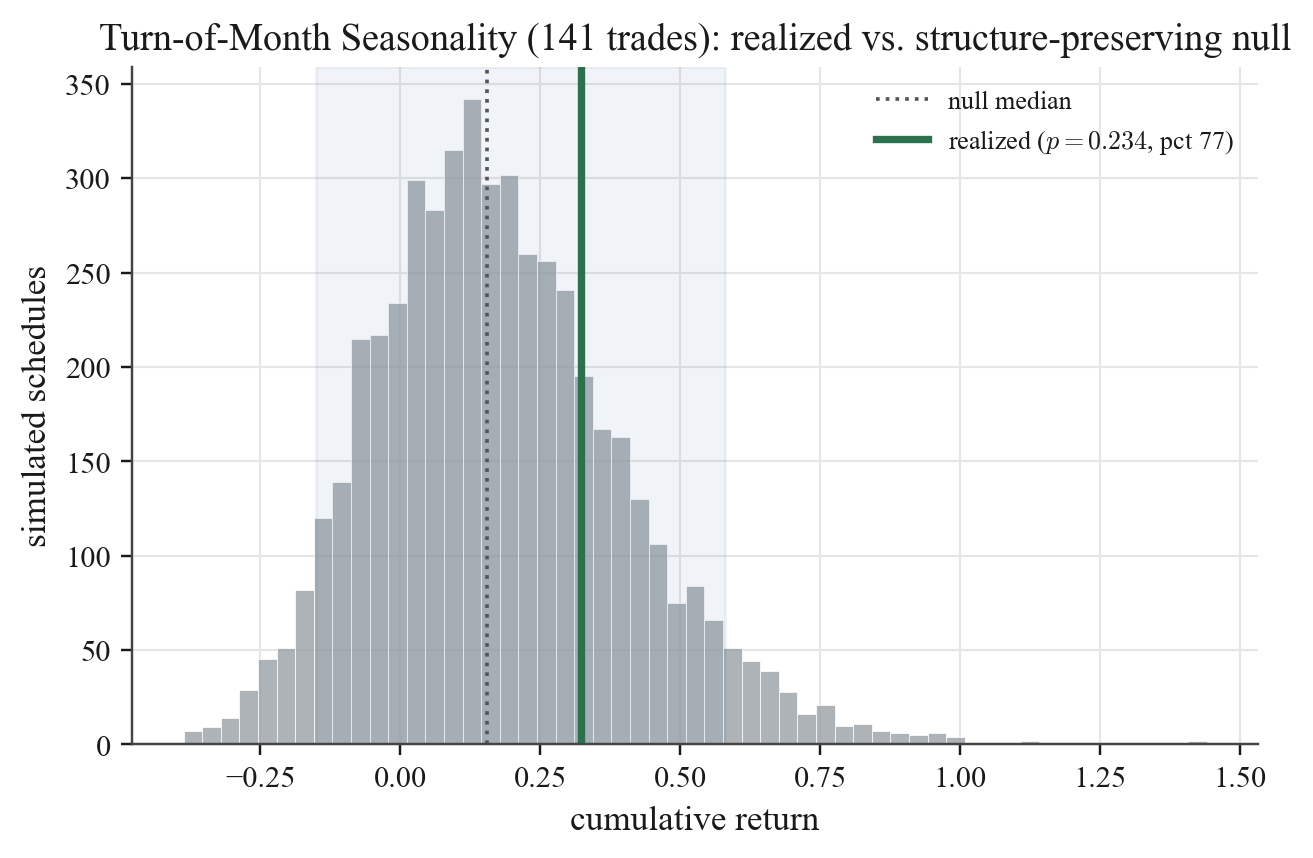
\includegraphics[width=0.72\textwidth]{mc_turn_of_month_seasonality.png}
\caption{GC=F. Monte Carlo distribution of final returns, Turn-of-Month (daily). Caption values: actual return = 0.3229; median simulated return = 0.1553; simulated 5th/95th = (-0.1498, 0.5794); p-value = 0.2336; actual percentile = 76.7; trades = 141; simulations = 5{,}000; transaction cost = 0.000470.}
\label{fig:mc_turnofmonth}
\end{figure}

\begin{figure}[htbp]
\centering
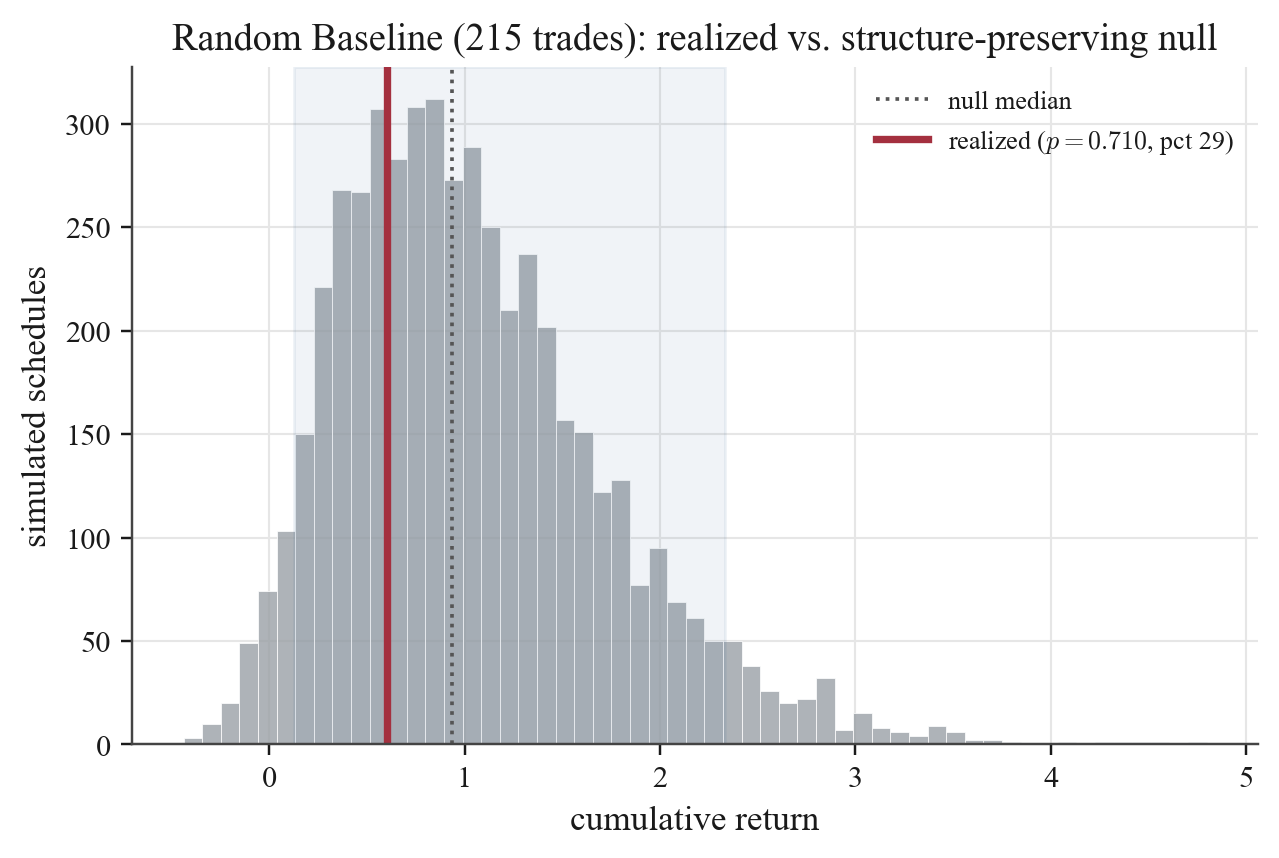
\includegraphics[width=0.72\textwidth]{mc_random.png}
\caption{GC=F. Monte Carlo distribution of final returns, Random strategy (daily). Caption values: actual return = 0.6011; median simulated return = 0.9381; simulated 5th/95th = (0.1276, 2.3314); p-value = 0.7103; actual percentile = 29.0; trades = 215; simulations = 5{,}000; transaction cost = 0.000470.}
\label{fig:mc_random}
\end{figure}

\begin{figure}[htbp]
\centering
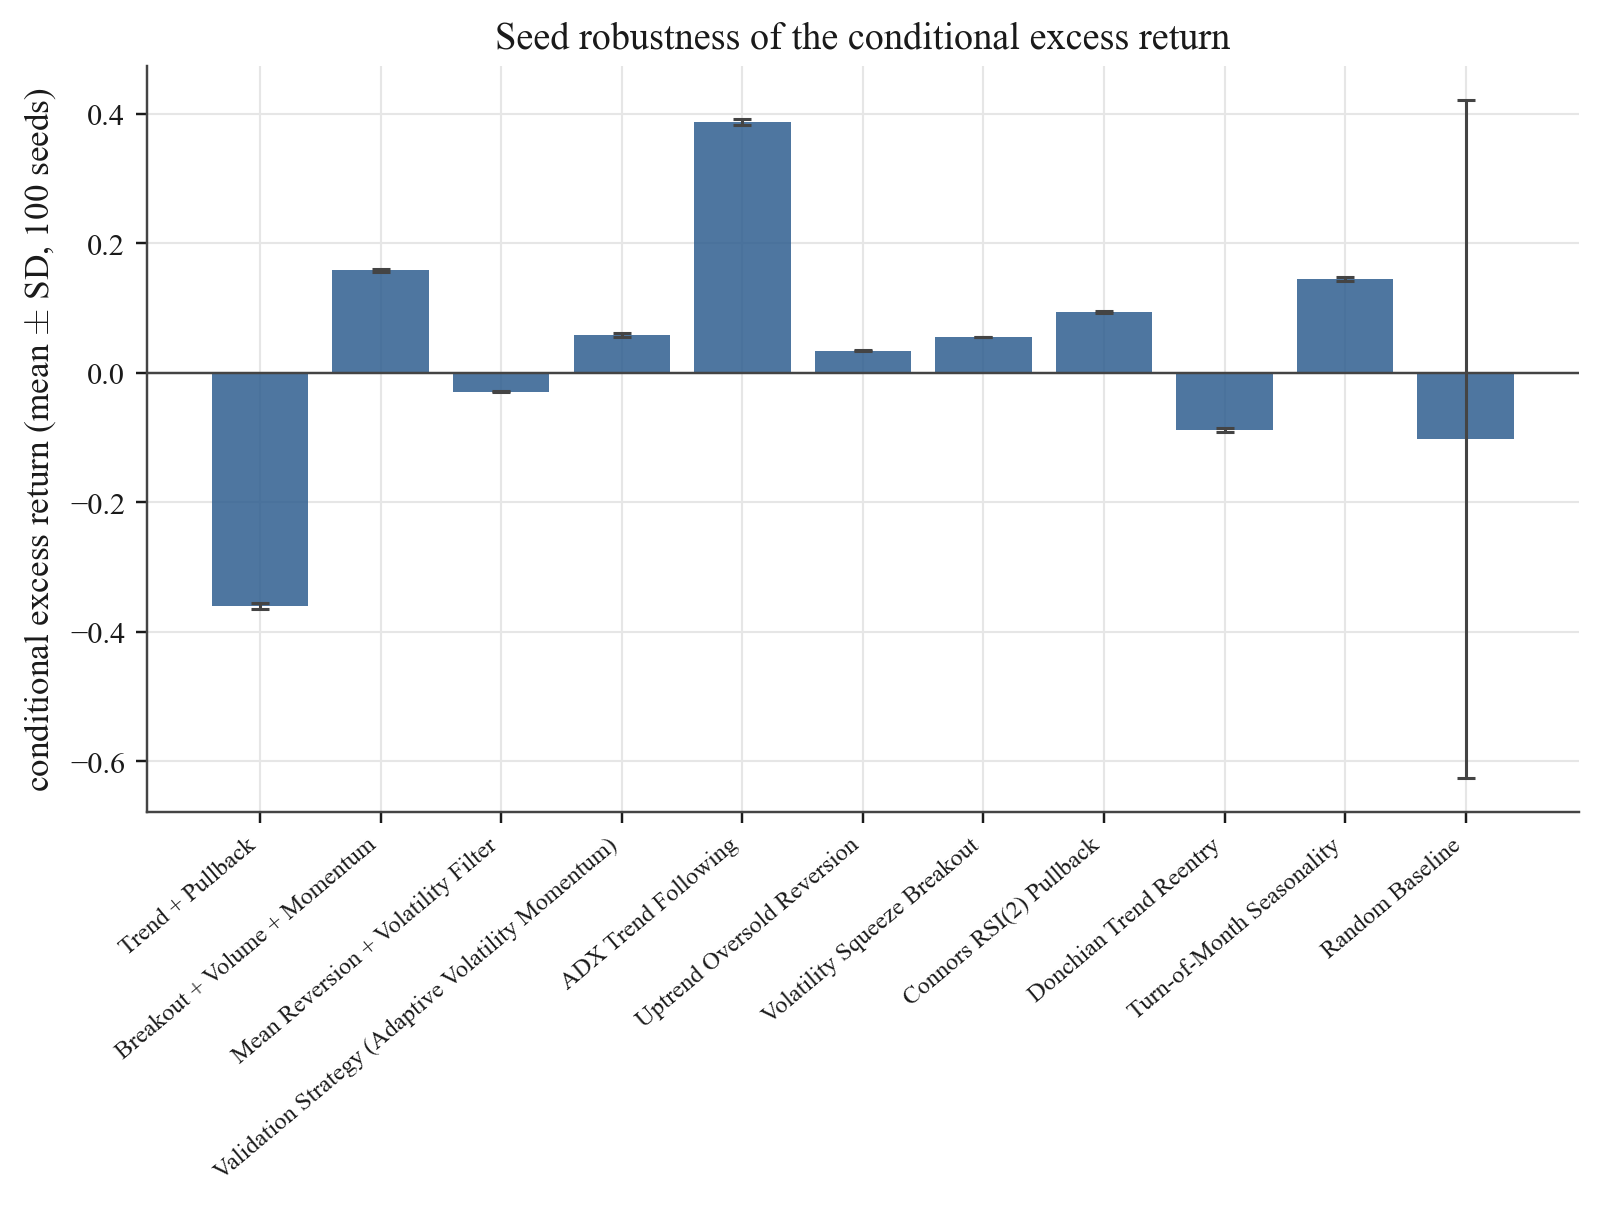
\includegraphics[width=0.85\textwidth]{rcsi_robustness.png}
\caption{GC=F. Monte Carlo robustness of RCSI across seeds (daily). The figure reports mean $\pm$ SD across outer runs, with outer runs = 100 and simulations per run = 5{,}000. Examples: Trend Pullback $-0.361\pm0.005$; ADX Trend $0.387\pm0.005$; Random $-0.103\pm0.523$. Transaction cost = 0.000470.}
\label{fig:rcsi_robust}
\end{figure}

\begin{figure}[htbp]
\centering
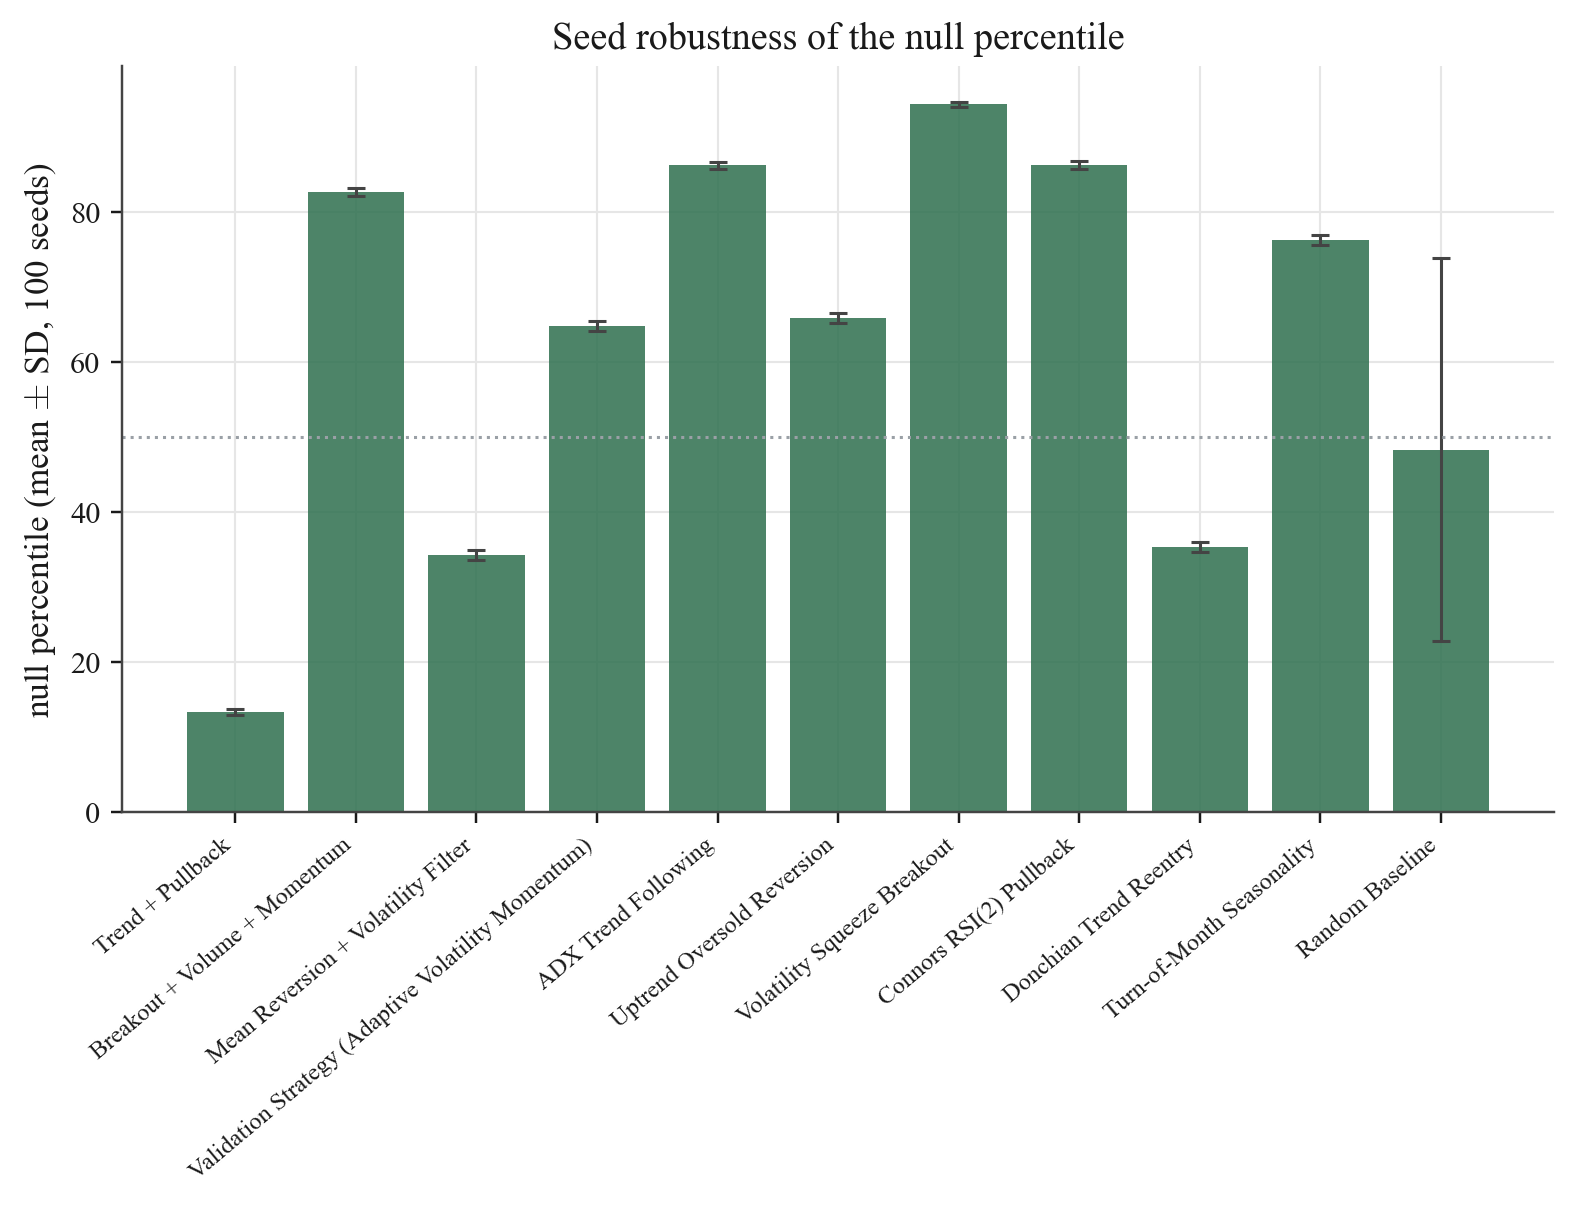
\includegraphics[width=0.85\textwidth]{percentile_robustness.png}
\caption{GC=F. Monte Carlo robustness of actual percentile across seeds (daily). Mean $\pm$ SD across outer runs. Examples: Squeeze Breakout $94.3\pm0.3$; ADX Trend $86.2\pm0.4$; Breakout Vol+Mom $82.7\pm0.5$; Random $48.3\pm25.6$.}
\label{fig:pct_robust}
\end{figure}

\begin{figure}[htbp]
\centering
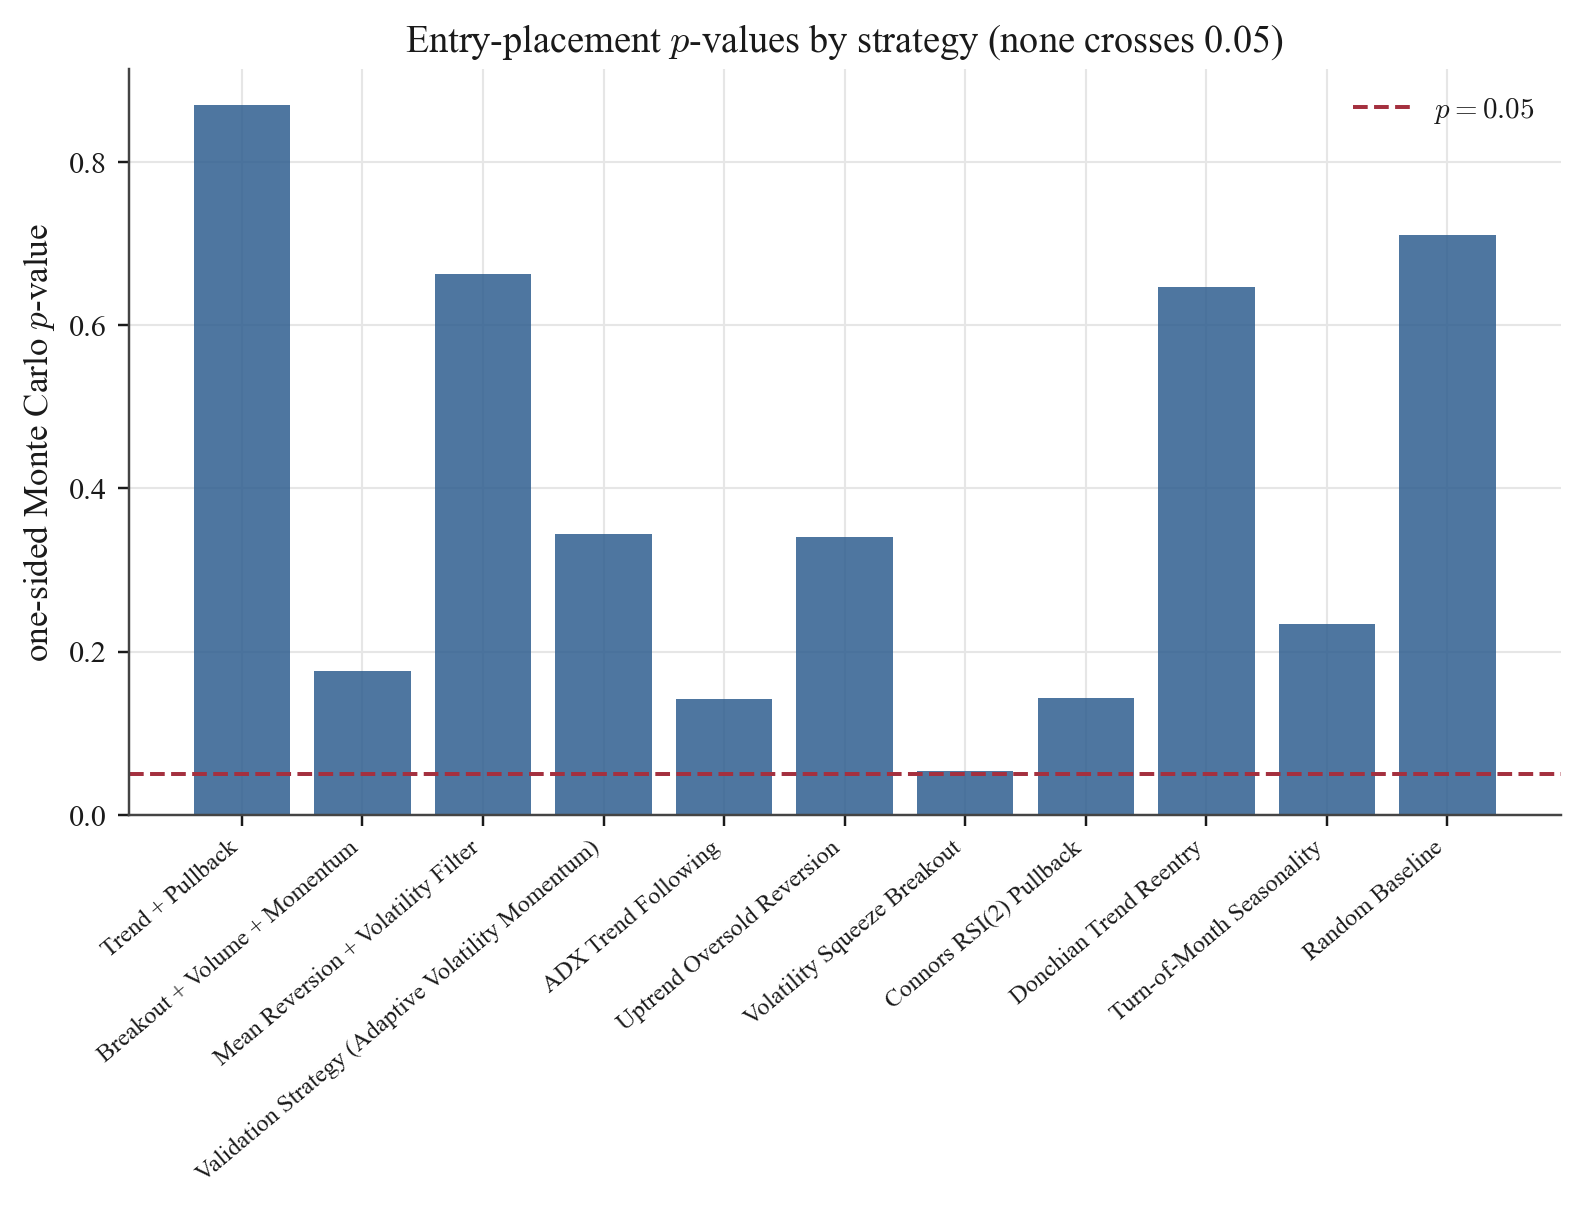
\includegraphics[width=0.85\textwidth]{pvalue_by_strategy.png}
\caption{GC=F. Monte Carlo p-value by strategy (daily). The dashed reference line marks the conventional threshold $p=0.05$. None of the plotted p-values crosses this threshold.}
\label{fig:pval_by_strategy}
\end{figure}

\begin{figure}[htbp]
\centering
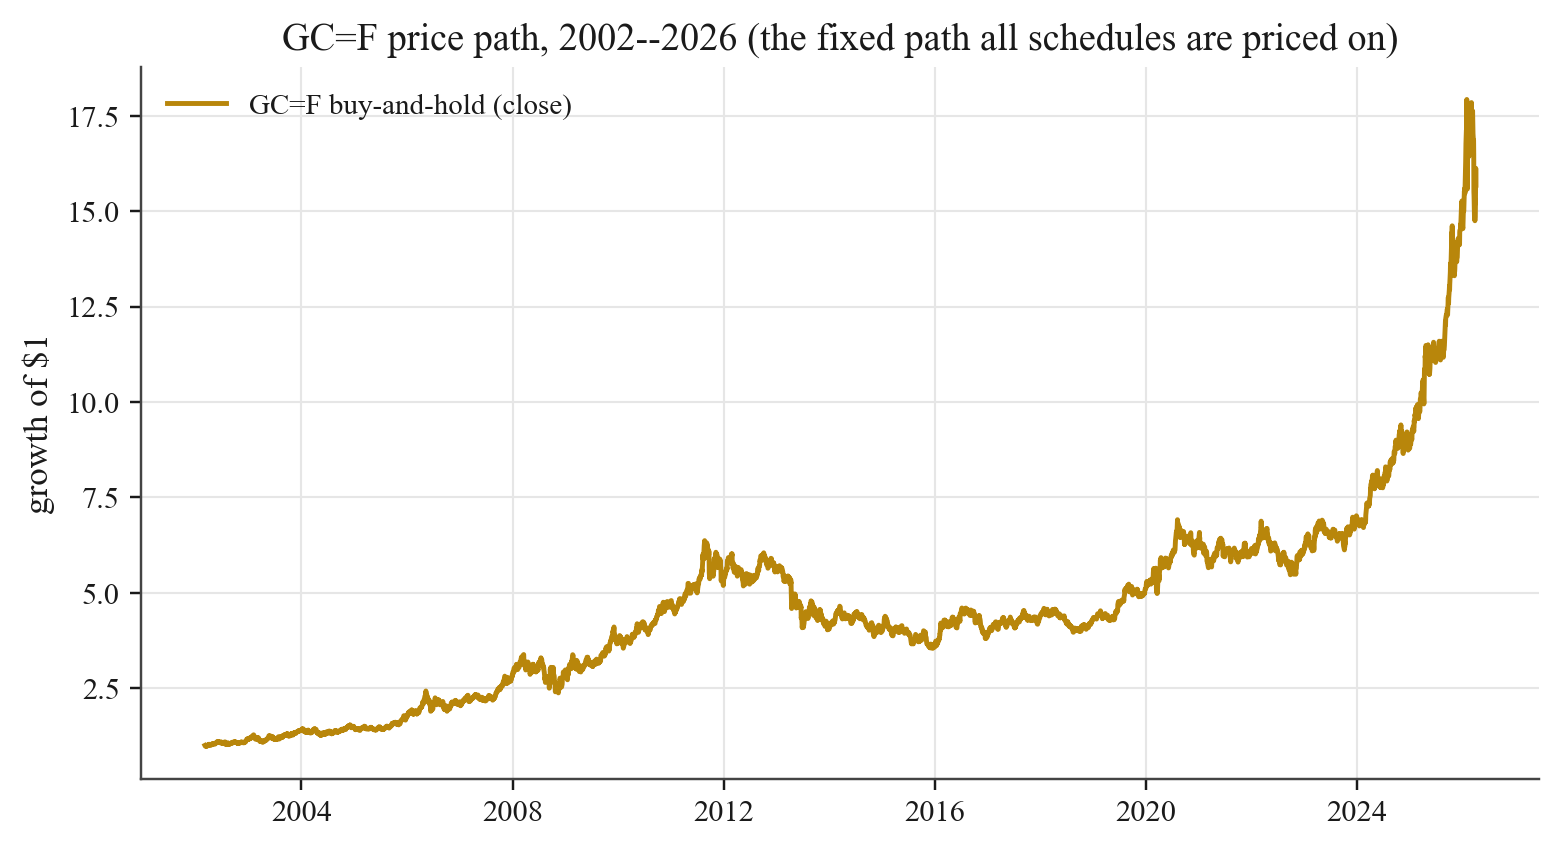
\includegraphics[width=0.85\textwidth]{equity_curve.png}
\caption{GC=F. Equity curves by strategy and benchmark (daily). Caption values list final cumulative returns: Trend Pullback 0.083; Breakout Vol+Mom 0.297; Mean Rev Vol Filter -0.010; Validation AVM 0.219; ADX Trend 0.803; Oversold Reversion 0.082; Squeeze Breakout 0.065; Connors RSI2 0.118; Donchian Reentry 0.071; Turn-of-Month 0.323; Random 0.601; Buy \& Hold 14.670. Sample window: 2002-03-04 00:00 to 2026-04-02 00:00.}
\label{fig:equity_curves}
\end{figure}


\section{Discussion}

\subsection{Skill versus luck in the empirical record}

The regime and Monte Carlo results support a disciplined interpretation of skill. Several strategies deliver positive returns yet sit near the center of their null distributions, a pattern well explained by chance timing under the same structural burden. A smaller subset occupies the right tail of the null with stable percentiles across seeds, indicating timing decisions that improve outcomes relative to structurally matched random placement, but not enough to clear strong significance thresholds in this experiment.

\subsection{What the framework changes}

The framework changes inference. It does not replace backtesting. It clarifies what a backtest means. A profitability-only view would rank most of these strategies as successful. The structure-preserving null asks a different question: whether the timing deserves credit. Under that question, the strategy panel produces:
\begin{itemize}
\item weak skill for a minority of strategies,
\item random or luck for a large share of profitable strategies,
\item below the null median for two strategies, including the stochastic Random baseline.
\end{itemize}

The Random baseline result is instructive. A strategy profitable at 0.601 sits at percentile 29.0 of its own null on the seed-42 realization, and at $48.3\pm 25.6$ across $R=100$ outer seeds, exactly as expected for a strategy with no entry-placement information. The single-seed verdict should not be read as ``negative skill''; the robust statement is that the random control is statistically indistinguishable from its own null, while still earning a sizable cumulative return from long exposure to a trending asset. This is the cleanest illustration of the gap the framework is designed to expose.

\subsection{Regime dependence and conditional skill}

The regime heatmap shows that performance is conditional. Breakout Vol+Mom is strongest in Stressed regimes at 0.29 (n=8), ADX Trend is strongest in Neutral regimes at 0.27 (n=60), and Validation AVM is strongest in Calm regimes at 0.34 (n=13). Squeeze Breakout is suppressed across all regimes because its trade count is too low. These patterns support a regime-sensitive interpretation of the local evidence while limiting claims about universal skill.

The regime results connect directly to the entry-placement interpretation. If the entry-placement advantage were universal, strategies would outperform random timing across all volatility environments. Instead, the evidence suggests that the advantage concentrates in specific regimes. This concentration is consistent with technical signals carrying regime-dependent information content: momentum and breakout signals are more informative in moderate-volatility environments where trends develop coherently, while mean-reversion signals require the low-volatility conditions that the regime filter selects for. Entry-placement evidence should therefore be evaluated regime-conditionally as well as in aggregate. Any strategy claiming universal edge deserves particular scrutiny.

\section{Limitations}

This paper is intentionally strict about what it claims, and several limitations should be acknowledged.

\textbf{Statistical power.} Evidence remains below the conventional $p \le 0.05$ threshold across the primary GC=F panel. This reflects genuinely absent skill, insufficient sample size, or both. Trade counts vary widely. Squeeze Breakout contributes only four trades in the GC=F analysis, which limits the power of the timing test for low-frequency strategies. The multi-asset walk-forward extension increases breadth, but it uses one outer run per panel and should therefore be read as external-validity evidence rather than seed-robust inference.

\textbf{Asset and frequency coverage.} The strongest empirical claims remain daily and long-only. The paper now includes an exploratory 14-instrument daily walk-forward extension and a bounded recent-frequency check on daily, 4-hour, and hourly bars, but it does not yet provide repeated seed-level robustness across all assets or a deep high-frequency universe. The framework itself is asset-agnostic and frequency-agnostic, but claims about broad market universality require deeper replication.

\textbf{Long-only restriction.} The current panel evaluates only long-only strategies. The structure-preserving null generalizes to short or mixed-direction strategies, but the empirical results here do not address timing skill in short-selling contexts.

\textbf{Between-strategy specification search.} The structure-preserving null is a \emph{within-strategy} test. It does not, by itself, correct for the fact that the eleven strategies in the panel were chosen by a researcher with knowledge of the literature and, in some cases, with prior exposure to the asset's history. We report Benjamini--Hochberg FDR-adjusted $p$-values, but we do not implement White's Reality Check, Hansen's SPA test, or Romano--Wolf stepdown inference in this empirical application. The deeper protection requires pre-registration or out-of-sample replication on assets and windows not used during rule design.

\textbf{Verified-output constraint.} The primary GC=F empirical section reports only the verified numeric outputs printed in the supplied figures. This improves source integrity but limits that analysis to metrics shown in those captions and tables. The simulation, benchmark-null, and multi-asset sections are generated from the accompanying code and are identified separately.

These limitations concern both the empirical application and the interpretation of the conditional null. The structure-preserving randomization requires no parametric return model and can expose profitable strategies whose realized entry placement is ordinary relative to structurally matched random timing, as the Random baseline demonstrates. It should nevertheless be read as a conditional diagnostic rather than a universal proof of skill or no skill. The framework applies mechanically to other assets, frequencies, and directions, but its conclusions scale only with the breadth, power, and out-of-sample discipline of the evidence.

\section{Conclusion}

This paper advances a simple but consequential claim: the relevant object of inference in strategy evaluation is not profit in isolation, but the contribution of decisions relative to a counterfactual. A trading rule does not select the return-generating process. It selects when exposure is assumed. The structure-preserving Monte Carlo framework developed here tests the entry-placement margin by holding fixed trade count, holding-period structure, spacing, direction, and the observed price path while randomizing only entry timing. The contribution is not a rejection of backtesting but a refinement of its evidentiary meaning. A backtest describes realized performance. It does not, on its own, establish that the entry placement which produced that performance reflects genuine edge.

Applied to daily GC=F over 2002-03-04 to 2026-04-02, the framework yields a clear empirical conclusion within that sample. Profitability is common across the strategy panel, yet strong statistical evidence of entry-placement skill is not. No strategy crosses the conventional threshold of $p \le 0.05$, and none qualifies as moderate or strong skill. Four strategies classify as weak skill, five are better interpreted as random or luck, and two fall below the null median in the seed-42 run. That conclusion survives a leading-gap feasibility restriction unchanged, but it does not survive a change of schedule measure: under a context-matched null four strategies reject, and no strategy is significant under both measures. The honest reading is therefore the absence of \emph{robust} entry-placement skill---a verdict that holds under one defensible measure and reverses under another is null-sensitive, not general skill. The profit--skill divergence is systematic: strategies that appear successful under a profitability-only evaluation are often statistically ordinary, and never measure-invariant, once subjected to the structure-preserving null. Synthetic validation confirms the test itself is sound---calibrated at the nominal level with uniform null $p$-values, and monotone power against injected entry signal---so these are properties of the strategies, not of a mis-sized test. A positive control on the real gold path reinforces this: injecting genuine timing skill into the same procedure moves it from a calibrated null baseline to certain rejection ($\mathrm{RCSI}_z$ above $7$), so the null verdict is not a powerless test on real prices. At breadth, pooling all $322$ completed strategy-by-asset tests across $47$ instruments yields zero discoveries under Benjamini--Hochberg or Bonferroni control, with random baselines among the most extreme results---the profit--skill divergence does not resolve into skill even when many assets are scanned with honest multiplicity correction. The exploratory multi-asset walk-forward extension points in the same direction: across 712 strategy-fold panels, no strategy has a mean panel $p$-value below 0.49 or a broad stable entry-placement advantage. The bounded frequency check is consistent with that conclusion: neither the daily nor 4-hour recent panels produce broad significance, and the lone favorable hourly mean-reversion result remains positive but inconclusive.

This paper proposes not only a method but a stricter standard for evaluating trading strategies. The conventional approach (report a positive backtest return, a Sharpe ratio, and a drawdown statistic) provides no counterfactual and therefore no basis for causal attribution. The structure-preserving framework supplies that counterfactual. Strategy validation should move from outcome-based affirmation toward counterfactual timing-based inference, where any claim of edge must survive comparison with randomized implementations that preserve the strategy's structural burden. Under that standard, skill is not synonymous with profitability; entry-placement skill is demonstrated only when realized entry placement systematically exceeds what randomized placement on the same path would generate.

Future work should extend this framework to seed-robust multi-asset and deeper intraday panels, incorporate short and mixed-direction strategies, develop regime-conditional null distributions, broaden the conditioning set to release exit logic and holding-period choice as additional testable margins, and formalize the relationship between the structure-preserving null and existing multiple-testing corrections for joint inference across strategy panels. The conclusion follows directly from the evidence presented here, within the scope it covers: profitability alone does not identify entry-placement edge.

\appendix

\section{Execution and fill model}
\label{app:execution}

Each strategy begins with \$100{,}000 of capital. The default maximum capital allocation per trade is $100\%$ of available capital, and the liquidity cap is $5\%$ of $20$-bar average volume. Non-crypto assets are traded in integer share quantities, while crypto assets are traded in increments of $0.0001$ units. Entry and exit fills are adverse to the trader: the reference price is the next-bar open, the half-spread is $0.5$ basis points, slippage on each side is drawn uniformly from $0.5$ to $3.0$ basis points, and the per-order commission for non-forex, non-crypto assets is $\max(0.005\times\text{shares},\,\$1)$. A candidate entry is rejected if no later bar remains for exit, if the next open gaps through the intended stop or target before the position is established, or if position size is infeasible after applying the capital and liquidity constraints. Positions do not overlap within a strategy; when both the stop-loss and take-profit are touched within the same bar, the stop-loss path is taken conservatively; and any surviving open position is liquidated at the last available open in the sample. The Monte Carlo null reprices each simulated schedule under this same model---a half-spread of $0.5$ basis points, a fresh per-side slippage draw on $[0.5,3.0]$ basis points, and an expected commission rate of $0.00002$---so that the realized strategy and its null comparison paths face identical frictions. Together these imply the expected round-trip cost $c=0.000470$ used throughout.

\section{Strategy rule definitions}
\label{app:strategy_rules}

The eleven reported strategies are implemented as follows.
\begin{itemize}
\item \textbf{Trend Pullback.} Entry requires the 50-bar moving average to exceed the 200-bar moving average, the close to exceed the 50-bar moving average, ADX to be at least 18, a pullback to or through the 20-bar exponential moving average, RSI(14) in the interval \([35,65]\), and a close at least as high as the previous close. The stop is the minimum of the current low and the lagged 10-bar low, less one ATR. The target is the lagged 20-bar high, with a fallback 2:1 reward-to-risk target if that level is not above the signal close. Exit occurs on stop, target, or failure of the long-horizon trend filter.

\item \textbf{Breakout Vol+Mom.} Entry requires either a close above the lagged 20-bar high or a near-breakout close within 0.2\% of that level, together with a participation filter, a momentum filter, and ADX of at least 18. Participation is defined by a volume ratio of at least 1.1 when volume is informative, or by a range-expansion condition of at least \(1.03\times\) ATR otherwise. Momentum is defined by MACD above its signal line or a 12-bar return of at least 0.5\%. The stop is the minimum of the current low and the lagged 10-bar low, less one ATR. The target is set at a 2:1 reward-to-risk multiple. Exit occurs on stop, target, failed breakout, or a 15-bar time stop.

\item \textbf{Mean Rev Vol Filter.} Entry requires a non-stressed, low-volatility, low-trend environment: ADX below 25, either the ATR ratio or the Bollinger-width ratio no greater than 1.6, and an absolute distance from the 50-bar moving average no greater than 3\%. The oversold trigger is the current low at or below the lower Bollinger band within a 0.2\% buffer, together with RSI(14) no greater than 35. The stop is the minimum of the current low and the lagged 5-bar low, less one ATR. The target is the Bollinger midpoint. Exit occurs on stop, target, reversion to the midpoint, or RSI recovery to at least 50.

\item \textbf{Validation AVM.} Entry requires the close above the 200-bar moving average, the 50-bar moving average at or above the 200-bar moving average, positive 20-bar and 60-bar returns, MACD above its signal line, ADX of at least 10, RSI(14) in \([45,82]\), an ATR ratio no greater than 1.9, a non-stressed regime, and either a reclaim of the 20-bar exponential moving average or a breakout above the lagged 20-bar high with volume confirmation. The stop is the lower of the lagged breakout low and the signal close minus \(2.2\times \mathrm{ATR}\). The target is the signal close plus \(6.0\times \mathrm{ATR}\). Position size is additionally scaled inversely with the ATR ratio, floored at 35\% and capped at 100\% of available capital. Exit occurs on stop, target, trailing stop, volatility shock, trend or momentum breakdown, or an 80-bar time stop.

\item \textbf{ADX Trend.} Entry requires the close above the 200-bar moving average, the 50-bar moving average at or above the 200-bar moving average, a positive 20-bar return, positive directional dominance, ADX of at least 18 and rising, an ATR ratio no greater than 2.2, and a non-stressed regime. The stop is the minimum of the lagged 10-bar low and the signal close minus \(2.0\times \mathrm{ATR}\). The target is the signal close plus \(4.0\times \mathrm{ATR}\). Exit occurs on stop, target, a reversal defined by the close below the 20-bar exponential moving average together with negative directional dominance, or a 90-bar time stop.

\item \textbf{Oversold Reversion.} Entry requires the close above the 200-bar moving average, the 50-bar moving average at or above the 200-bar moving average, a 20-bar price \(z\)-score no greater than \(-1.2\), either a touch of the lower Bollinger band or RSI(14) no greater than 40, a close at least as high as the previous close, and a non-stressed regime. The stop is the minimum of the current low and the signal close minus \(1.5\times \mathrm{ATR}\). The target is the signal close plus \(2.5\times \mathrm{ATR}\). Exit occurs on stop, target, recovery to the 20-bar exponential moving average, or a 20-bar time stop.

\item \textbf{Squeeze Breakout.} Entry requires volatility compression, defined by a Bollinger-width ratio no greater than 0.85, a breakout above the lagged 20-bar high, MACD above its signal line, ADX of at least 14, a volume ratio of at least 0.95 when volume is available, the close above the 200-bar moving average, and a non-stressed regime. The stop is the minimum of the lagged 10-bar low and the signal close minus \(1.8\times \mathrm{ATR}\). The target is the signal close plus \(3.5\times \mathrm{ATR}\). Exit occurs on stop, target, trailing stop, breakout failure, or a 45-bar time stop.

\item \textbf{Connors RSI2.} A Wilder-style RSI(2) and a 5-bar moving average are computed from closing prices. Entry requires the 50-bar moving average at or above the 200-bar moving average, the close above the 200-bar moving average, RSI(2) no greater than 5, a close no higher than the previous close, and a non-stressed regime. The stop is the minimum of the current low and the signal close minus \(1.5\times \mathrm{ATR}\). Exit occurs on stop, RSI(2) recovery to at least 70, recovery to the 5-bar moving average, break of the 200-bar trend filter, or an 8-bar time stop.

\item \textbf{Donchian Reentry.} Entry requires the close above the 200-bar moving average, the 50-bar moving average at or above the 200-bar moving average, a close above the lagged 55-bar Donchian high with no breakout on the previous bar, MACD at or above its signal line, ADX of at least 15, and a non-stressed regime. The stop is the minimum of the lagged 20-bar low and the signal close minus \(2.0\times \mathrm{ATR}\). The target is the signal close plus \(4.0\times \mathrm{ATR}\). Exit occurs on stop, target, loss of 50-bar trend support, momentum fade, or an 80-bar time stop.

\item \textbf{Turn-of-Month.} A signal is generated on the last trading day of each calendar month. Entry additionally requires a non-stressed regime and the close above the 200-bar moving average. The stop is the signal close minus \(2.0\times \mathrm{ATR}\). Exit occurs on stop, break of the trend filter, or completion of a fixed 4-bar holding window.

\item \textbf{Random.} This control strategy ignores market features. On each bar, entry occurs with probability 0.07, subject to the same feasibility, cost, sizing, and non-overlap rules as the rule-based strategies. At entry, the holding period is drawn uniformly from 4 to 18 bars, and exit occurs only when that planned holding period is reached. The main single-ticker run uses a fixed random seed of 42 for this baseline.
\end{itemize}

\section{Reproducibility appendix}

\textbf{Code and data availability.} All code and the derived data required to reproduce every table and figure in this paper are publicly available at \url{https://github.com/ampatel355/Fortuna} and permanently archived at \url{https://doi.org/10.5281/zenodo.20695539}. The repository contains the structure-preserving null implementation, the analysis scripts referenced in this appendix, the regime-labeled price series and realized trade logs, and a \texttt{README} mapping each table and figure to its exact reproduction command. Runs are deterministic under the seed protocol described below.

\subsection{Figure-based data sources}

The GC=F empirical panel---cumulative returns, trade counts, Monte Carlo $p$-values, percentiles, $\mathrm{RCSI}_z$, regime ratios, and seed robustness in Table~\ref{tab:main}---is reproduced directly from the canonical trade logs and the structure-preserving null by \texttt{Code/regenerate\_gallery.py} (Monte Carlo distributions, conditional excess, $p$-values, and regime ratios) and the robustness summary (seed-level dispersion); the gallery figures of the previous section are produced by the same script. The script verifies its regenerated statistics against the reported values and aborts on any material mismatch, so figures and text cannot silently diverge.

\subsection{Computed analyses and exact commands}

The computed analyses below are generated directly from the accompanying code rather than transcribed, and reproduce exactly. The synthetic validation (Table~\ref{tab:synthetic_validation}, Figures~\ref{fig:synthetic_calibration} and~\ref{fig:synthetic_power}) is produced, from base seed $9100$, by
\begin{verbatim}
SYNTHETIC_REPLICATIONS=1500 SYNTHETIC_POWER_REPLICATIONS=400 \
SYNTHETIC_SIMULATIONS=2000 \
  ./.venv/bin/python Code/synthetic_timing_experiments.py
\end{verbatim}
which writes \texttt{Data\_Clean/synthetic\_null\_validation\_summary.csv}. The schedule-measure sensitivity (Table~\ref{tab:schedule_sensitivity}) re-evaluates the fixed GC=F trade logs under each measure with $M=5{,}000$ simulations and the seed-$42$ spawn protocol:
\begin{verbatim}
MEASURE_LABEL=baseline \
  ./.venv/bin/python Code/schedule_measure_sensitivity.py
MONTE_CARLO_MIN_LEADING_INDEX=200 \
  MEASURE_LABEL=leading_gap_200 \
  ./.venv/bin/python Code/schedule_measure_sensitivity.py
MONTE_CARLO_CONTEXT_MATCHING=1 \
  MEASURE_LABEL=context_matched \
  ./.venv/bin/python Code/schedule_measure_sensitivity.py
\end{verbatim}
The baseline column reproduces Table~\ref{tab:main} exactly, confirming the harness matches the canonical pipeline; results are written to \texttt{Data\_Clean/\allowbreak GC=F\_sensitivity\_*.csv}.

The real-data positive control (Table~\ref{tab:positive_control}, Figures~\ref{fig:pc_curve} and~\ref{fig:pc_hist}) injects a tunable fraction of well-timed entries into a strategy on the GC=F open-price series and scores it against the structure-preserving null with execution-cost simulation disabled, over $100$ seeds at $M=5{,}000$:
\begin{verbatim}
  ./.venv/bin/python Code/positive_control_power.py
\end{verbatim}
which writes \texttt{Data\_Clean/\allowbreak GC=F\_positive\_control\_power\_summary.csv}. The cross-asset multiplicity panel (Table~\ref{tab:cross_asset_multiplicity}, Figure~\ref{fig:cross_asset}) aggregates the saved \texttt{Data\_Clean/*\_full\_comparison.csv} run outputs and applies Benjamini--Hochberg and Bonferroni control across all $322$ tests:
\begin{verbatim}
  ./.venv/bin/python Code/cross_asset_multiplicity.py
\end{verbatim}
which writes \texttt{Data\_Clean/cross\_asset\_panel\_summary.csv}. The realistic-signal detection results (Table~\ref{tab:signal_mechanisms}, Figure~\ref{fig:signal_curve}) and the regenerated GC=F figure gallery (Section~\ref{sec:figures-gallery}, Table~\ref{tab:main}) are produced by
\begin{verbatim}
  ./.venv/bin/python Code/positive_control_signals.py
  ./.venv/bin/python Code/regenerate_gallery.py
\end{verbatim}
The latter recomputes the eleven Monte Carlo distributions, the conditional excess, the $p$-values, and the regime ratios from the canonical trade logs and verifies them against the reported values before writing any figure.

\subsection{Statement on empirical integrity}

The GC=F empirical panel is reproduced from the canonical trade logs and the structure-preserving null by the commands in this appendix, which verify their regenerated statistics against the reported values and abort on any material mismatch; every value in the computed analyses is the direct output of those commands on the accompanying data. Where a quantity was produced by neither source, the paper states it qualitatively and does not invent a numeric estimate.

\bibliographystyle{elsarticle-num}

\begin{thebibliography}{99}

\bibitem{fama1970}
E. F. Fama, Efficient capital markets: A review of theory and empirical work,
\emph{The Journal of Finance} 25(2) (1970) 383--417.

\bibitem{lo2004}
A. W. Lo, The adaptive markets hypothesis: Market efficiency from an evolutionary perspective,
\emph{The Journal of Portfolio Management} 30(5) (2004) 15--29.

\bibitem{white2000}
H. White, A reality check for data snooping,
\emph{Econometrica} 68(5) (2000) 1097--1126.

\bibitem{hansen2005}
P. R. Hansen, A test for superior predictive ability,
\emph{Journal of Business \& Economic Statistics} 23(4) (2005) 365--380.

\bibitem{sullivan1999}
R. Sullivan, A. Timmermann, H. White, Data-snooping, technical trading rule performance, and the bootstrap,
\emph{The Journal of Finance} 54(5) (1999) 1647--1691.

\bibitem{bailey2017}
D. H. Bailey, J. M. Borwein, M. L\'opez de Prado, Q. J. Zhu,
The probability of backtest overfitting,
\emph{Journal of Computational Finance} 20(4) (2017) 39--69.

\bibitem{moskowitz2012}
T. J. Moskowitz, Y. H. Ooi, L. H. Pedersen, Time series momentum,
\emph{Journal of Financial Economics} 104(2) (2012) 228--250.

\bibitem{politisromano1994}
D. N. Politis, J. P. Romano, The stationary bootstrap,
\emph{Journal of the American Statistical Association} 89(428) (1994) 1303--1313.

\bibitem{benjaminihochberg1995}
Y. Benjamini, Y. Hochberg, Controlling the false discovery rate: A practical and powerful approach to multiple testing,
\emph{Journal of the Royal Statistical Society, Series B} 57(1) (1995) 289--300.

\bibitem{romanowolf2005}
J. P. Romano, M. Wolf, Stepwise multiple testing as formalized data snooping,
\emph{Econometrica} 73(4) (2005) 1237--1282.

\bibitem{harveyliuzhu2016}
C. R. Harvey, Y. Liu, H. Zhu, $\ldots$ and the cross-section of expected returns,
\emph{Review of Financial Studies} 29(1) (2016) 5--68.

\bibitem{lopezdeprado2018}
M. L\'opez de Prado, \emph{Advances in Financial Machine Learning}, Wiley, 2018.

\bibitem{baileylopez2014}
D. H. Bailey, M. L\'opez de Prado, The deflated Sharpe ratio: Correcting for selection bias, backtest overfitting, and non-normality,
\emph{Journal of Portfolio Management} 40(5) (2014) 94--107.

\bibitem{Fisher1935}
R. A. Fisher, \emph{The Design of Experiments}, Oliver \& Boyd, Edinburgh, 1935.

\bibitem{LehmannRomano2005}
E. L. Lehmann, J. P. Romano, \emph{Testing Statistical Hypotheses}, 3rd Edition, Springer, New York, 2005.

\bibitem{Candes2018}
E. Cand\`es, Y. Fan, L. Janson, J. Lv, Panning for gold: `model-X' knockoffs for high dimensional controlled variable selection,
\emph{Journal of the Royal Statistical Society: Series B} 80(3) (2018) 551--577.

\bibitem{Ernst2004}
M. D. Ernst, Permutation methods: A basis for exact inference,
\emph{Statistical Science} 19(4) (2004) 676--685.

\bibitem{Aldous1985}
D. J. Aldous, Exchangeability and related topics, in: \emph{\'Ecole d'\'Et\'e de Probabilit\'es de Saint-Flour XIII---1983}, Lecture Notes in Mathematics, vol.~1117, Springer, Berlin, 1985, pp.~1--198.

\bibitem{Dwass1957}
M. Dwass, Modified randomization tests for nonparametric hypotheses,
\emph{The Annals of Mathematical Statistics} 28(1) (1957) 181--187.

\bibitem{Hope1968}
A. C. A. Hope, A simplified Monte Carlo significance test procedure,
\emph{Journal of the Royal Statistical Society: Series B} 30(3) (1968) 582--598.

\bibitem{HemerikGoeman2018}
J. Hemerik, J. Goeman, Exact testing with random permutations,
\emph{TEST} 27(4) (2018) 811--825.

\bibitem{PhipsonSmyth2010}
B. Phipson, G. K. Smyth, Permutation $p$-values should never be zero: Calculating exact $p$-values when permutations are randomly drawn,
\emph{Statistical Applications in Genetics and Molecular Biology} 9(1) (2010) Article 39.

\bibitem{BesagClifford1989}
J. Besag, P. Clifford, Generalized Monte Carlo significance tests,
\emph{Biometrika} 76(4) (1989) 633--642.

\bibitem{PesarinSalmaso2010}
F. Pesarin, L. Salmaso, \emph{Permutation Tests for Complex Data: Theory, Applications and Software}, John Wiley \& Sons, Chichester, 2010.

\bibitem{FithianSunTaylor2014}
W. Fithian, D. Sun, J. Taylor, Optimal inference after model selection,
arXiv:1410.2597 (2014).

\bibitem{LeeSunSunTaylor2016}
J. D. Lee, D. L. Sun, Y. Sun, J. E. Taylor, Exact post-selection inference, with application to the lasso,
\emph{The Annals of Statistics} 44(3) (2016) 907--927.

\bibitem{BerkBrownBujaZhangZhao2013}
R. Berk, L. Brown, A. Buja, K. Zhang, L. Zhao, Valid post-selection inference,
\emph{The Annals of Statistics} 41(2) (2013) 802--837.

\bibitem{Kunsch1989}
H. R. K\"unsch, The jackknife and the bootstrap for general stationary observations,
\emph{The Annals of Statistics} 17(3) (1989) 1217--1241.

\bibitem{Storey2002}
J. D. Storey, A direct approach to false discovery rates,
\emph{Journal of the Royal Statistical Society: Series B} 64(3) (2002) 479--498.

\bibitem{BenjaminiYekutieli2001}
Y. Benjamini, D. Yekutieli, The control of the false discovery rate in multiple testing under dependency,
\emph{The Annals of Statistics} 29(4) (2001) 1165--1188.

\end{thebibliography}

\end{document}
